% \chapter{Appendix I}
% \label{sec:appendix}
% \blindtext[3]
%
% \chapter{Appendix II}
% \label{sec:appendix2}
% \blindtext[3]

\chapter{Appendix P-State Latencies}
\label{app:pstate_latencies_scatter_complete}
This section includes the scatter plots for all measurement points from the ftalat benchmark as described in~\secref{pstate_latencies}.

\begin{figure}[]
    \centering
    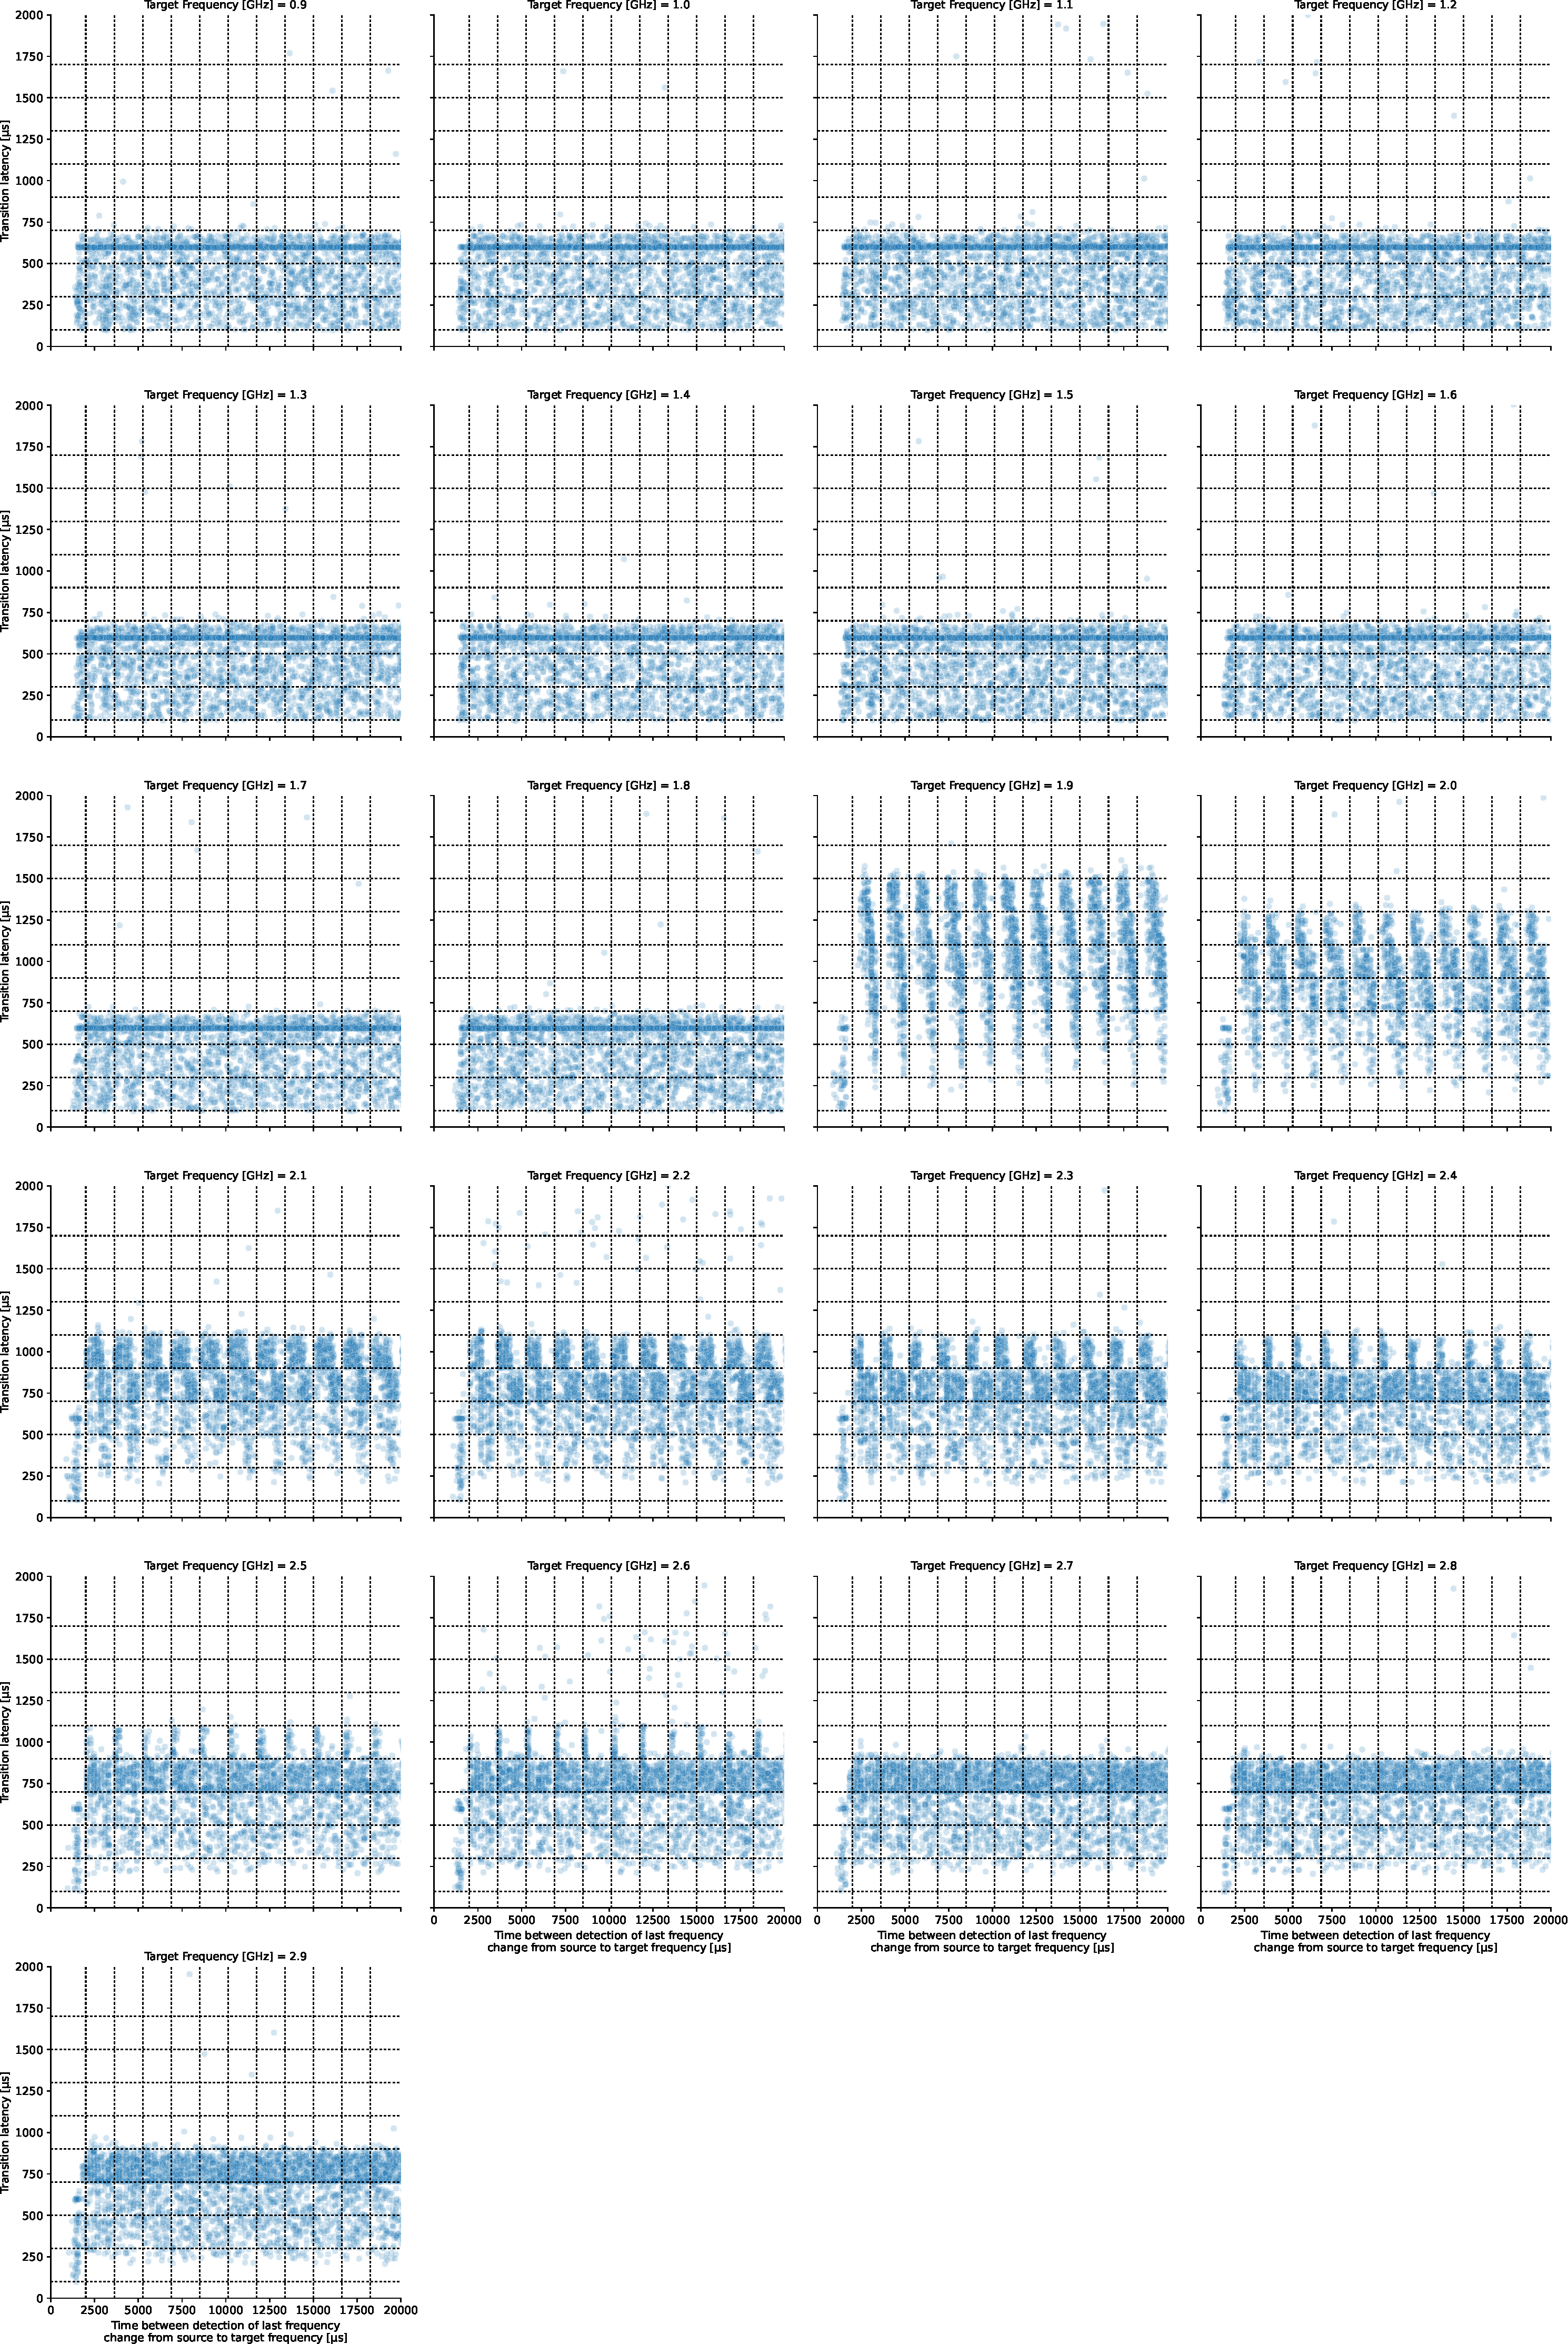
\includegraphics[width=\columnwidth]{fig/ftalat_scatter_wait_transition_latency_hati_source_0.8.pdf}
    \caption{Dependance of the time between the detection events of transitions from \SI{0.8}{\GHz} to \SI{0.9}{}, \SI{1.0}{}, ..., \SI{2.9}{\GHz}. For better lines for bins of size \SI{1625}{\us} and \SI{200}{\us} have been included for the x and y-axis respectively.}
\end{figure}
\begin{figure}[]
    \centering
    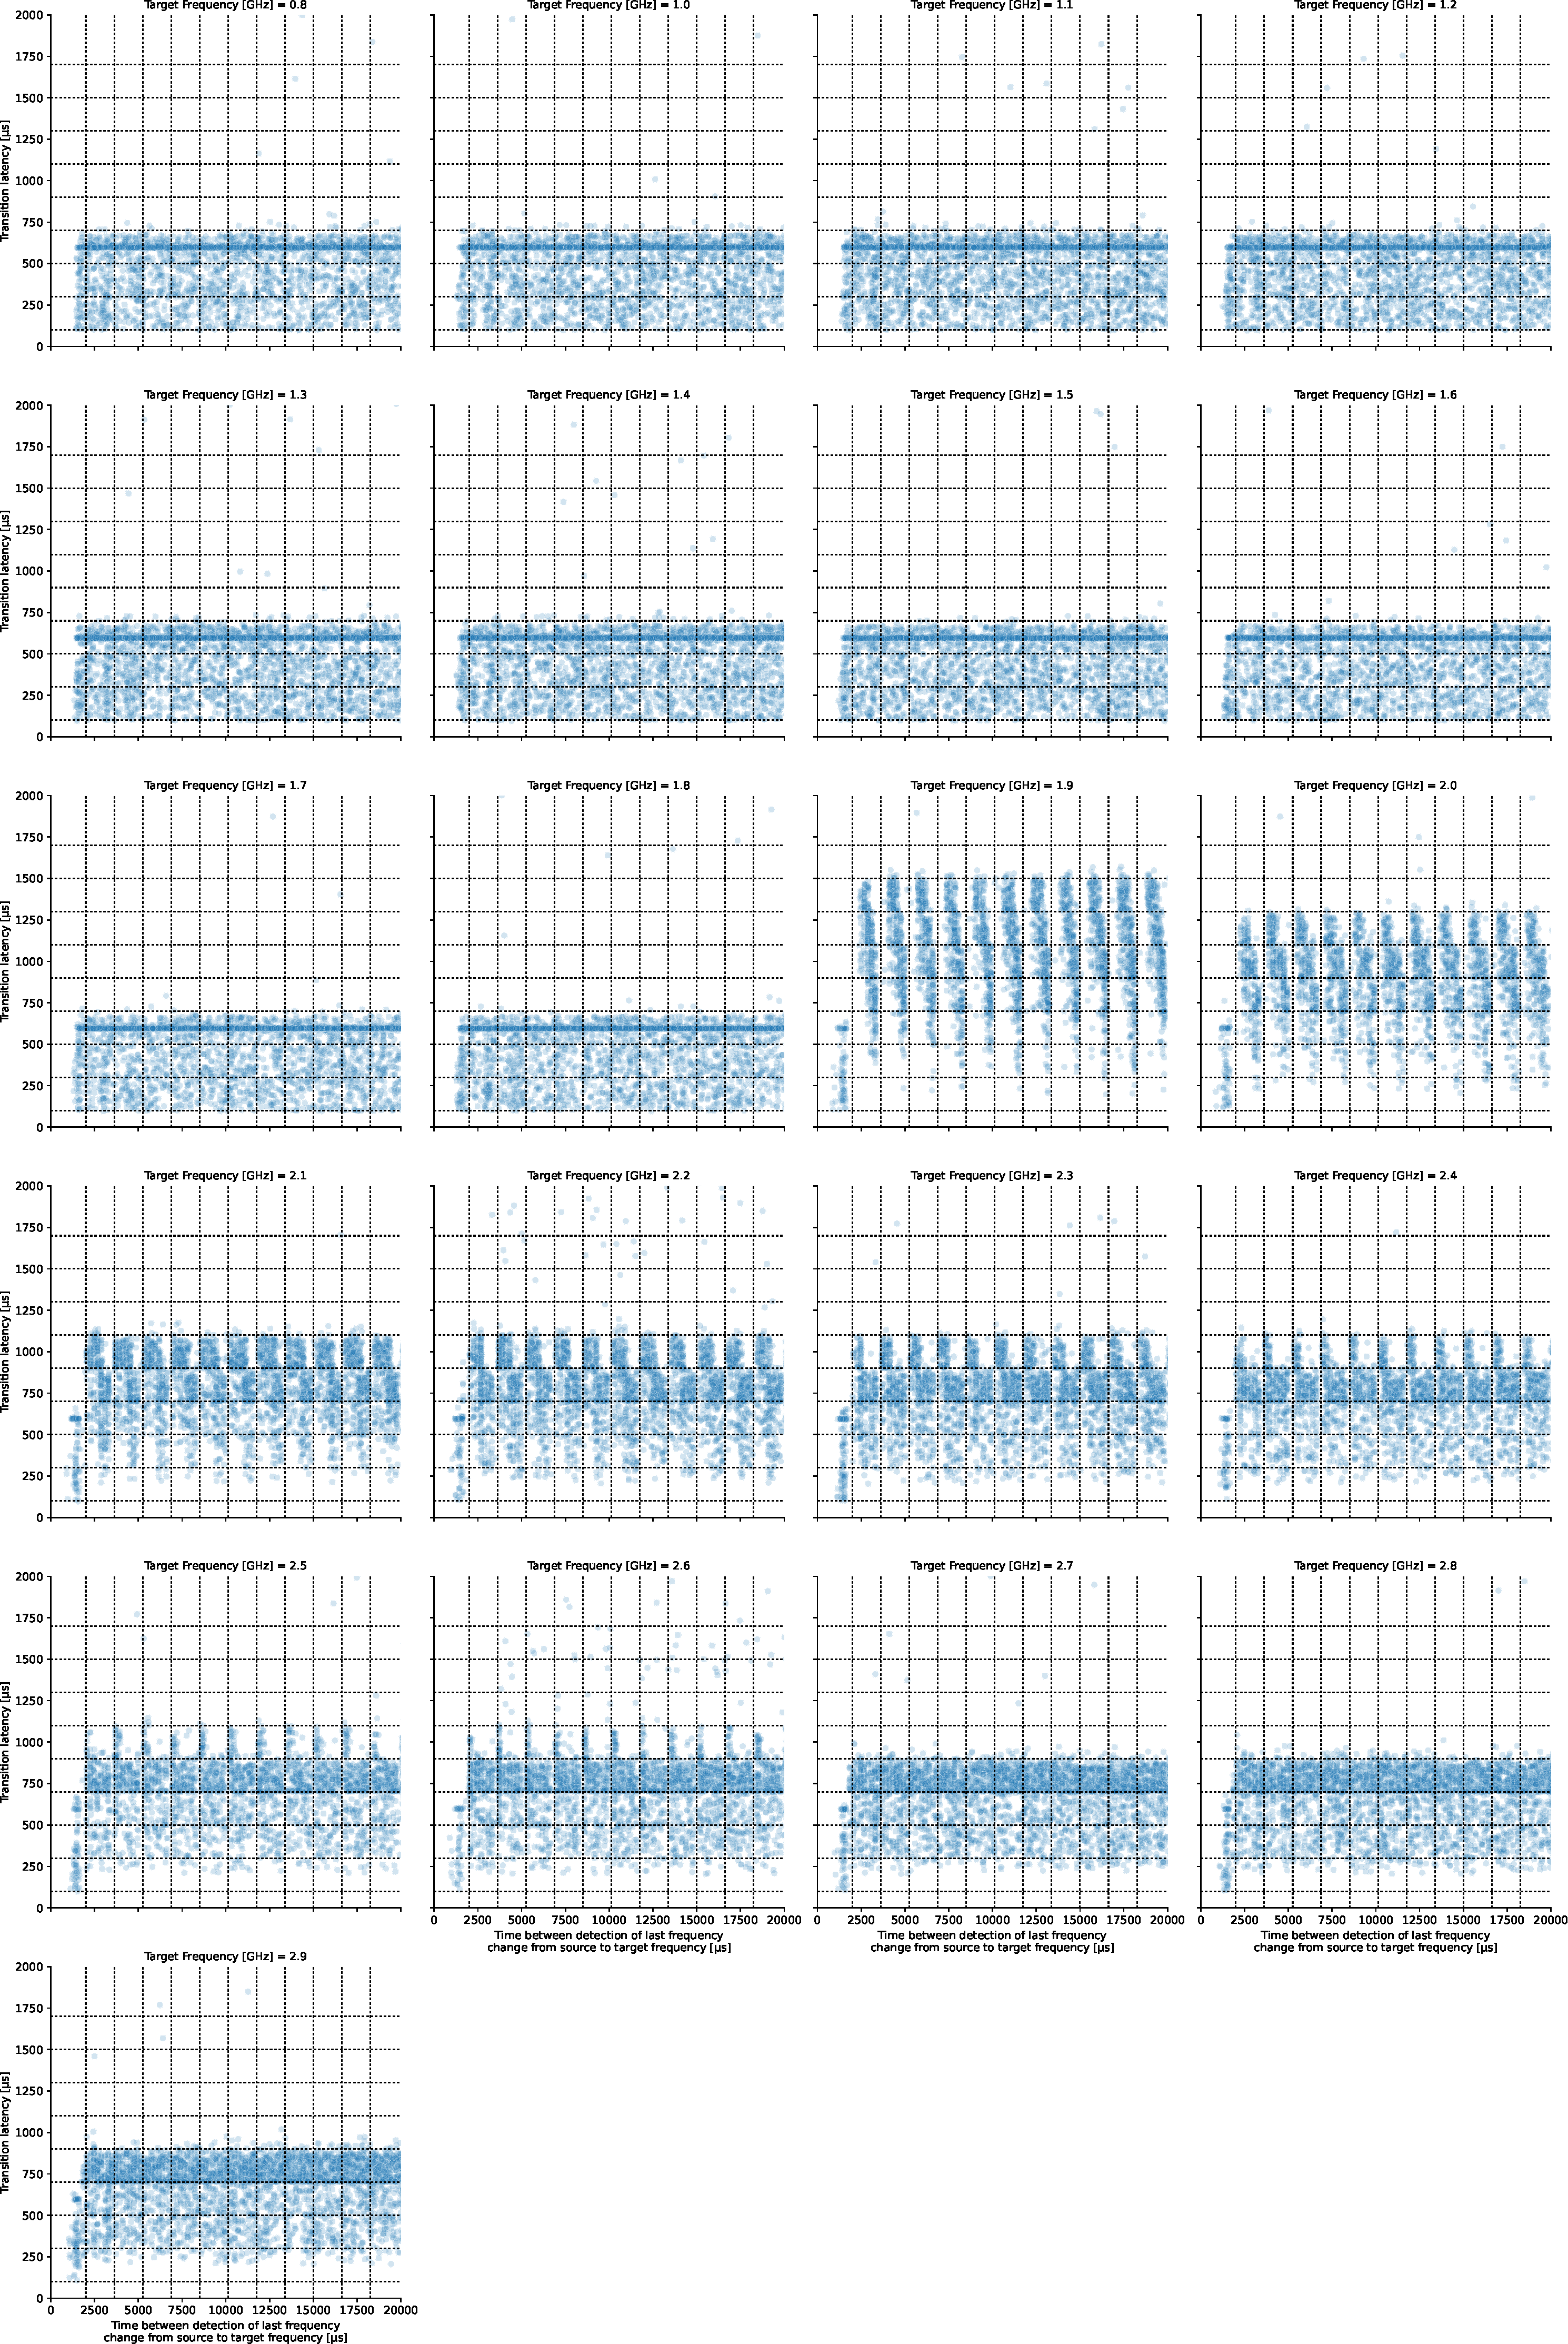
\includegraphics[width=\columnwidth]{fig/ftalat_scatter_wait_transition_latency_hati_source_0.9.pdf}
    \caption{Dependance of the time between the detection events of transitions from \SI{0.9}{\GHz} to \SI{0.8}{}, \SI{1.0}{}, ..., \SI{2.9}{\GHz}. For better lines for bins of size \SI{1625}{\us} and \SI{200}{\us} have been included for the x and y-axis respectively.}
\end{figure}
\begin{figure}[]
    \centering
    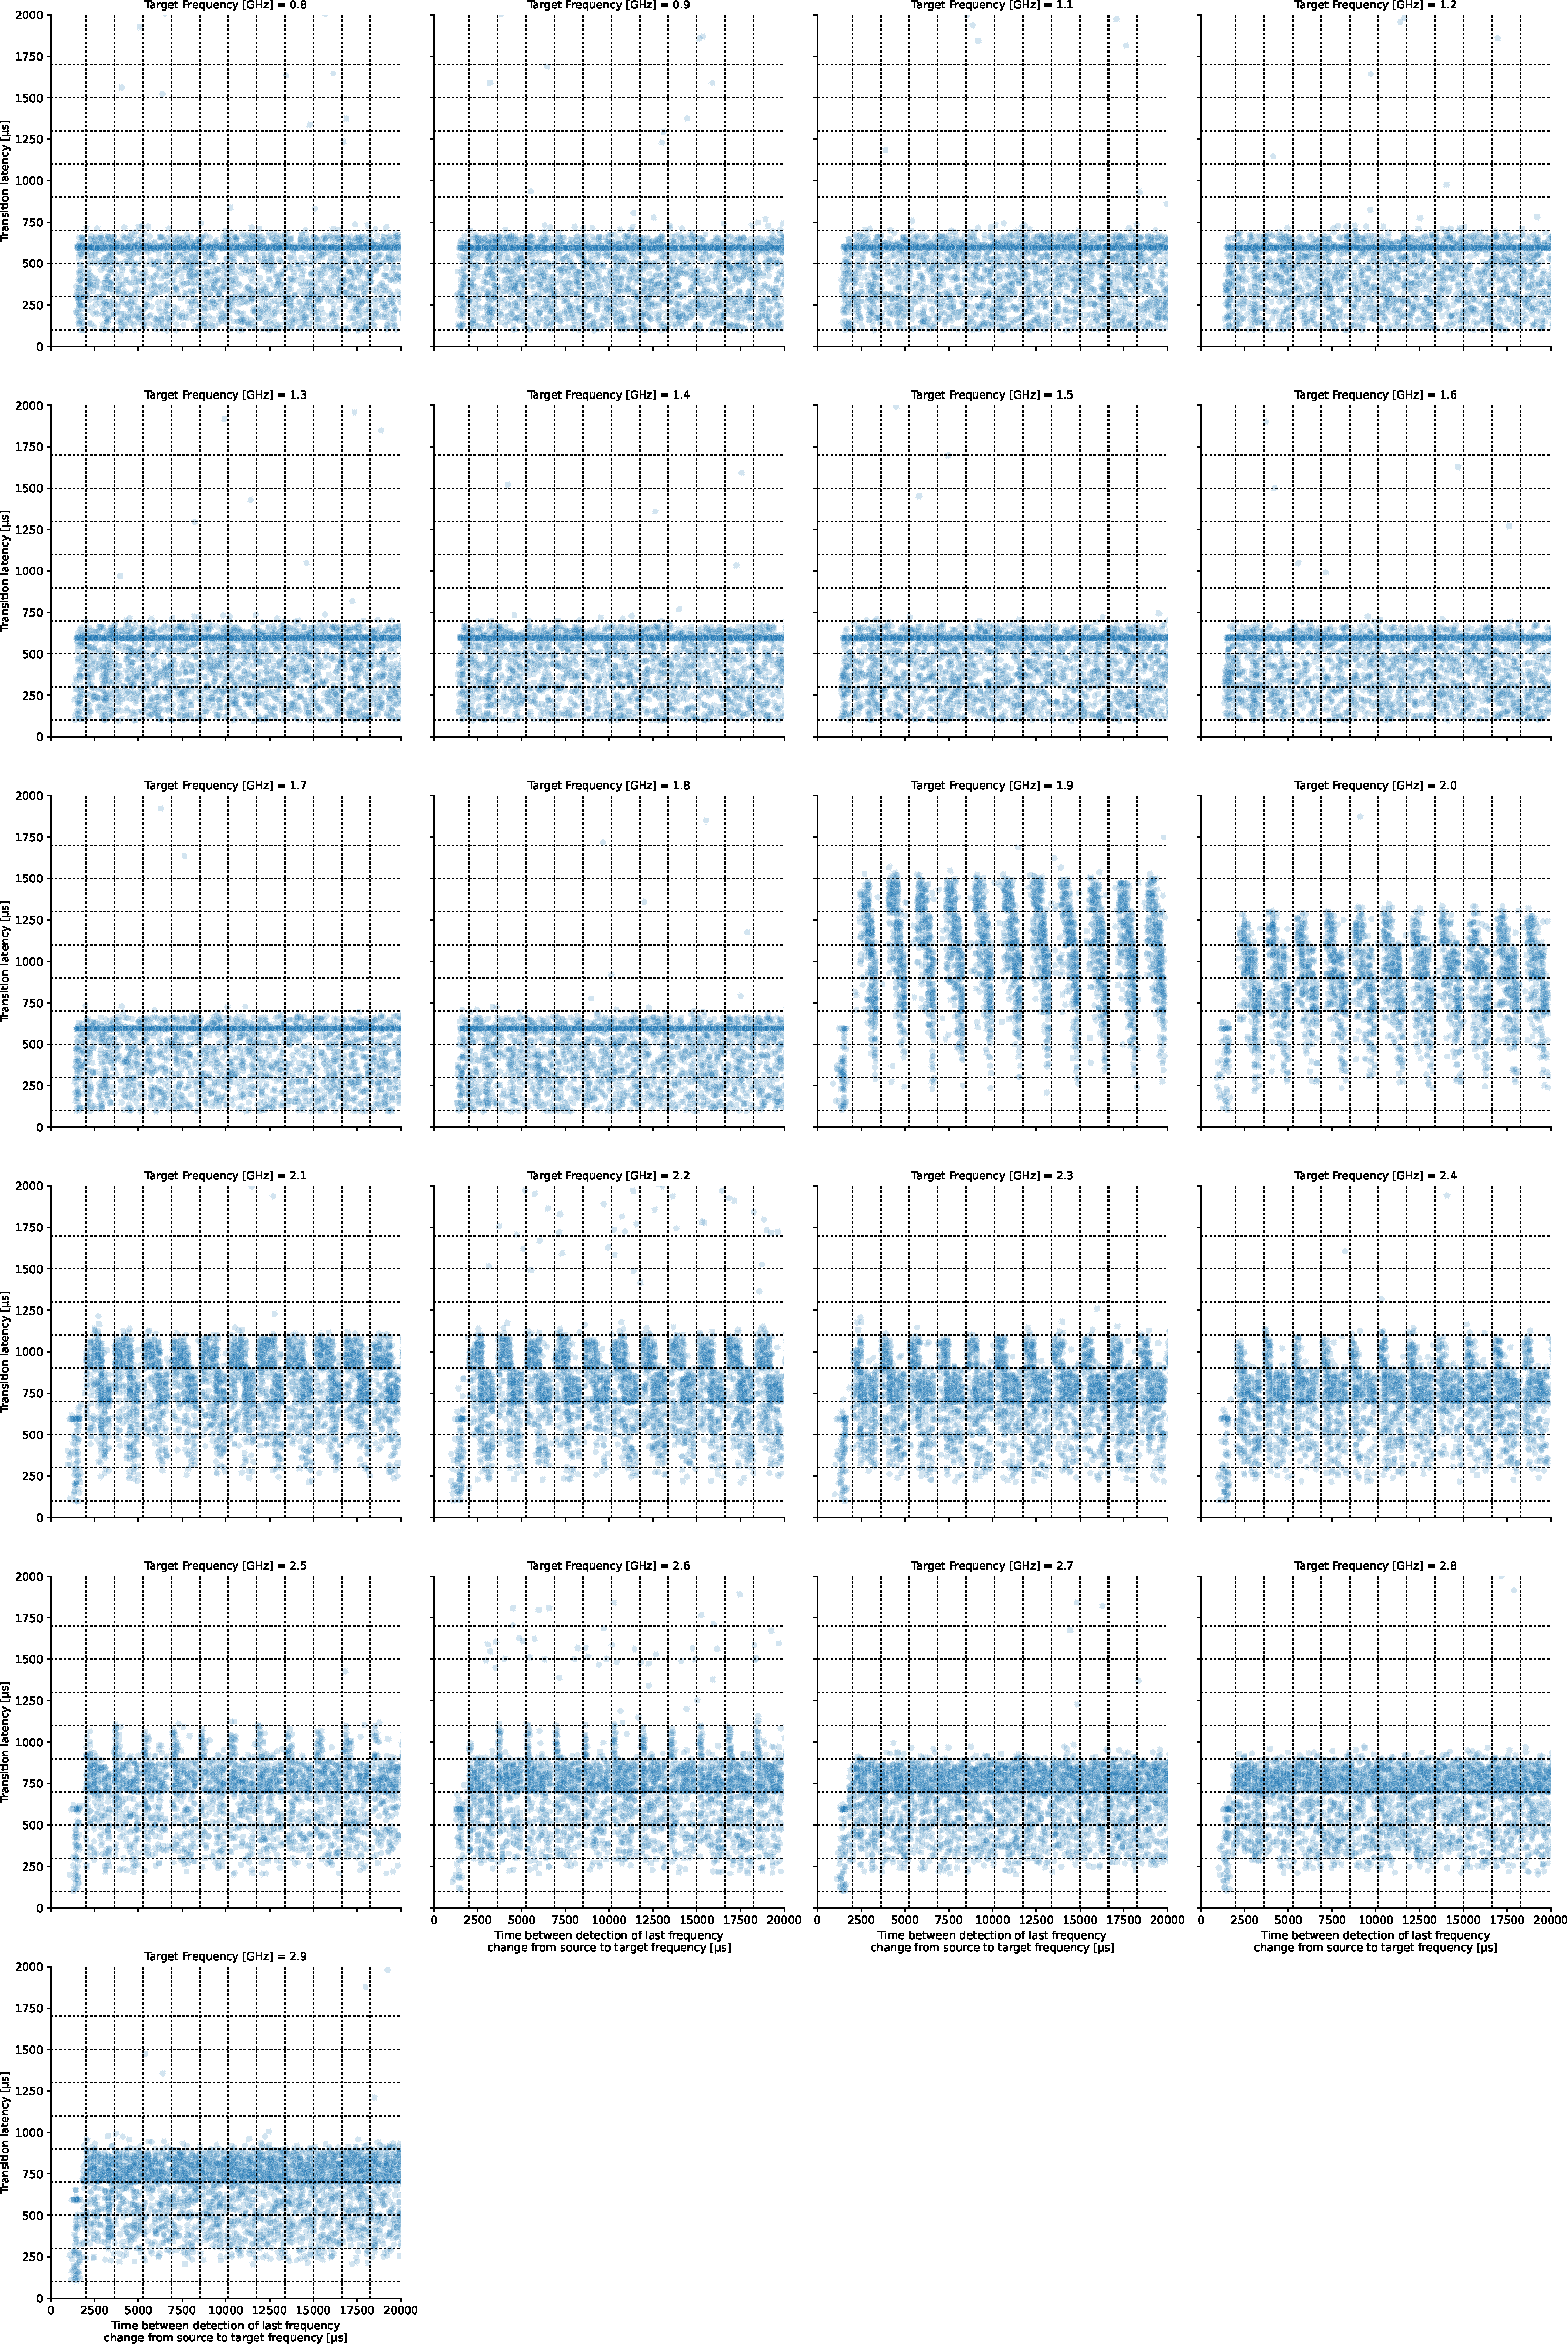
\includegraphics[width=\columnwidth]{fig/ftalat_scatter_wait_transition_latency_hati_source_1.0.pdf}
    \caption{Dependance of the time between the detection events of transitions from \SI{1.0}{\GHz} to \SI{0.8}{}, \SI{0.9}{}, ..., \SI{2.9}{\GHz}. For better lines for bins of size \SI{1625}{\us} and \SI{200}{\us} have been included for the x and y-axis respectively.}
\end{figure}
\begin{figure}[]
    \centering
    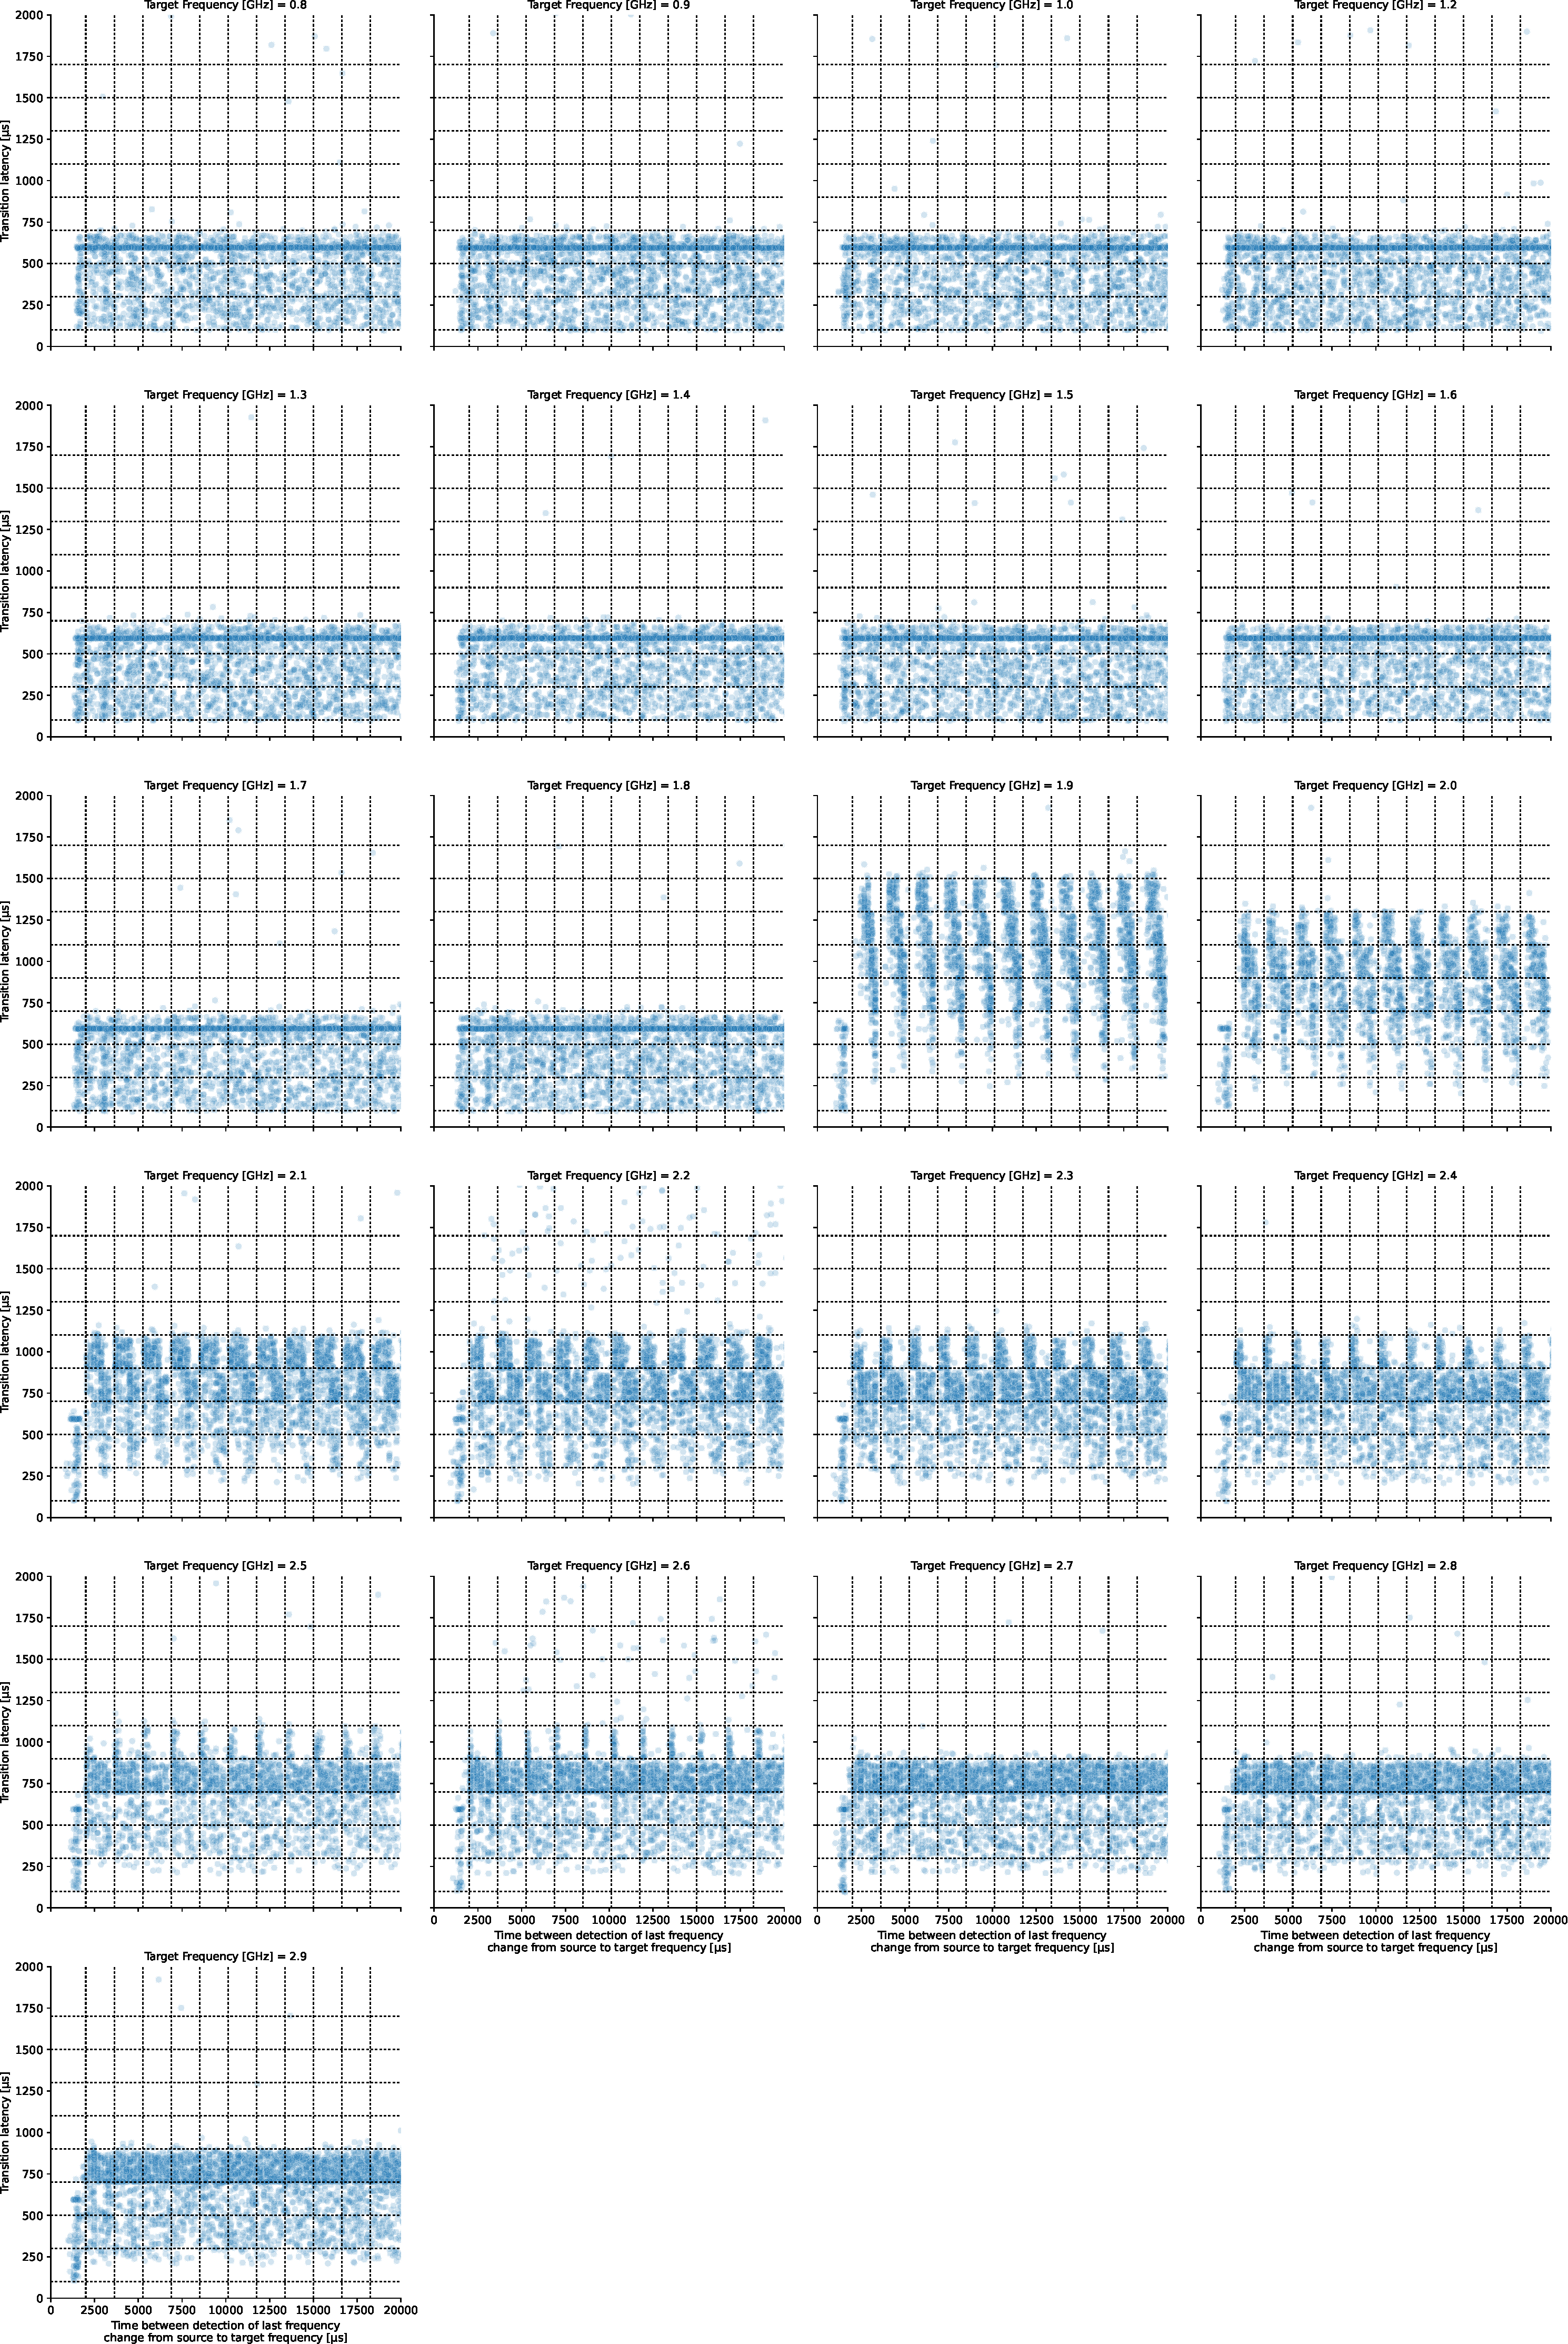
\includegraphics[width=\columnwidth]{fig/ftalat_scatter_wait_transition_latency_hati_source_1.1.pdf}
    \caption{Dependance of the time between the detection events of transitions from \SI{1.1}{\GHz} to \SI{0.8}{}, \SI{0.9}{}, ..., \SI{2.9}{\GHz}. For better lines for bins of size \SI{1625}{\us} and \SI{200}{\us} have been included for the x and y-axis respectively.}
\end{figure}
\begin{figure}[]
    \centering
    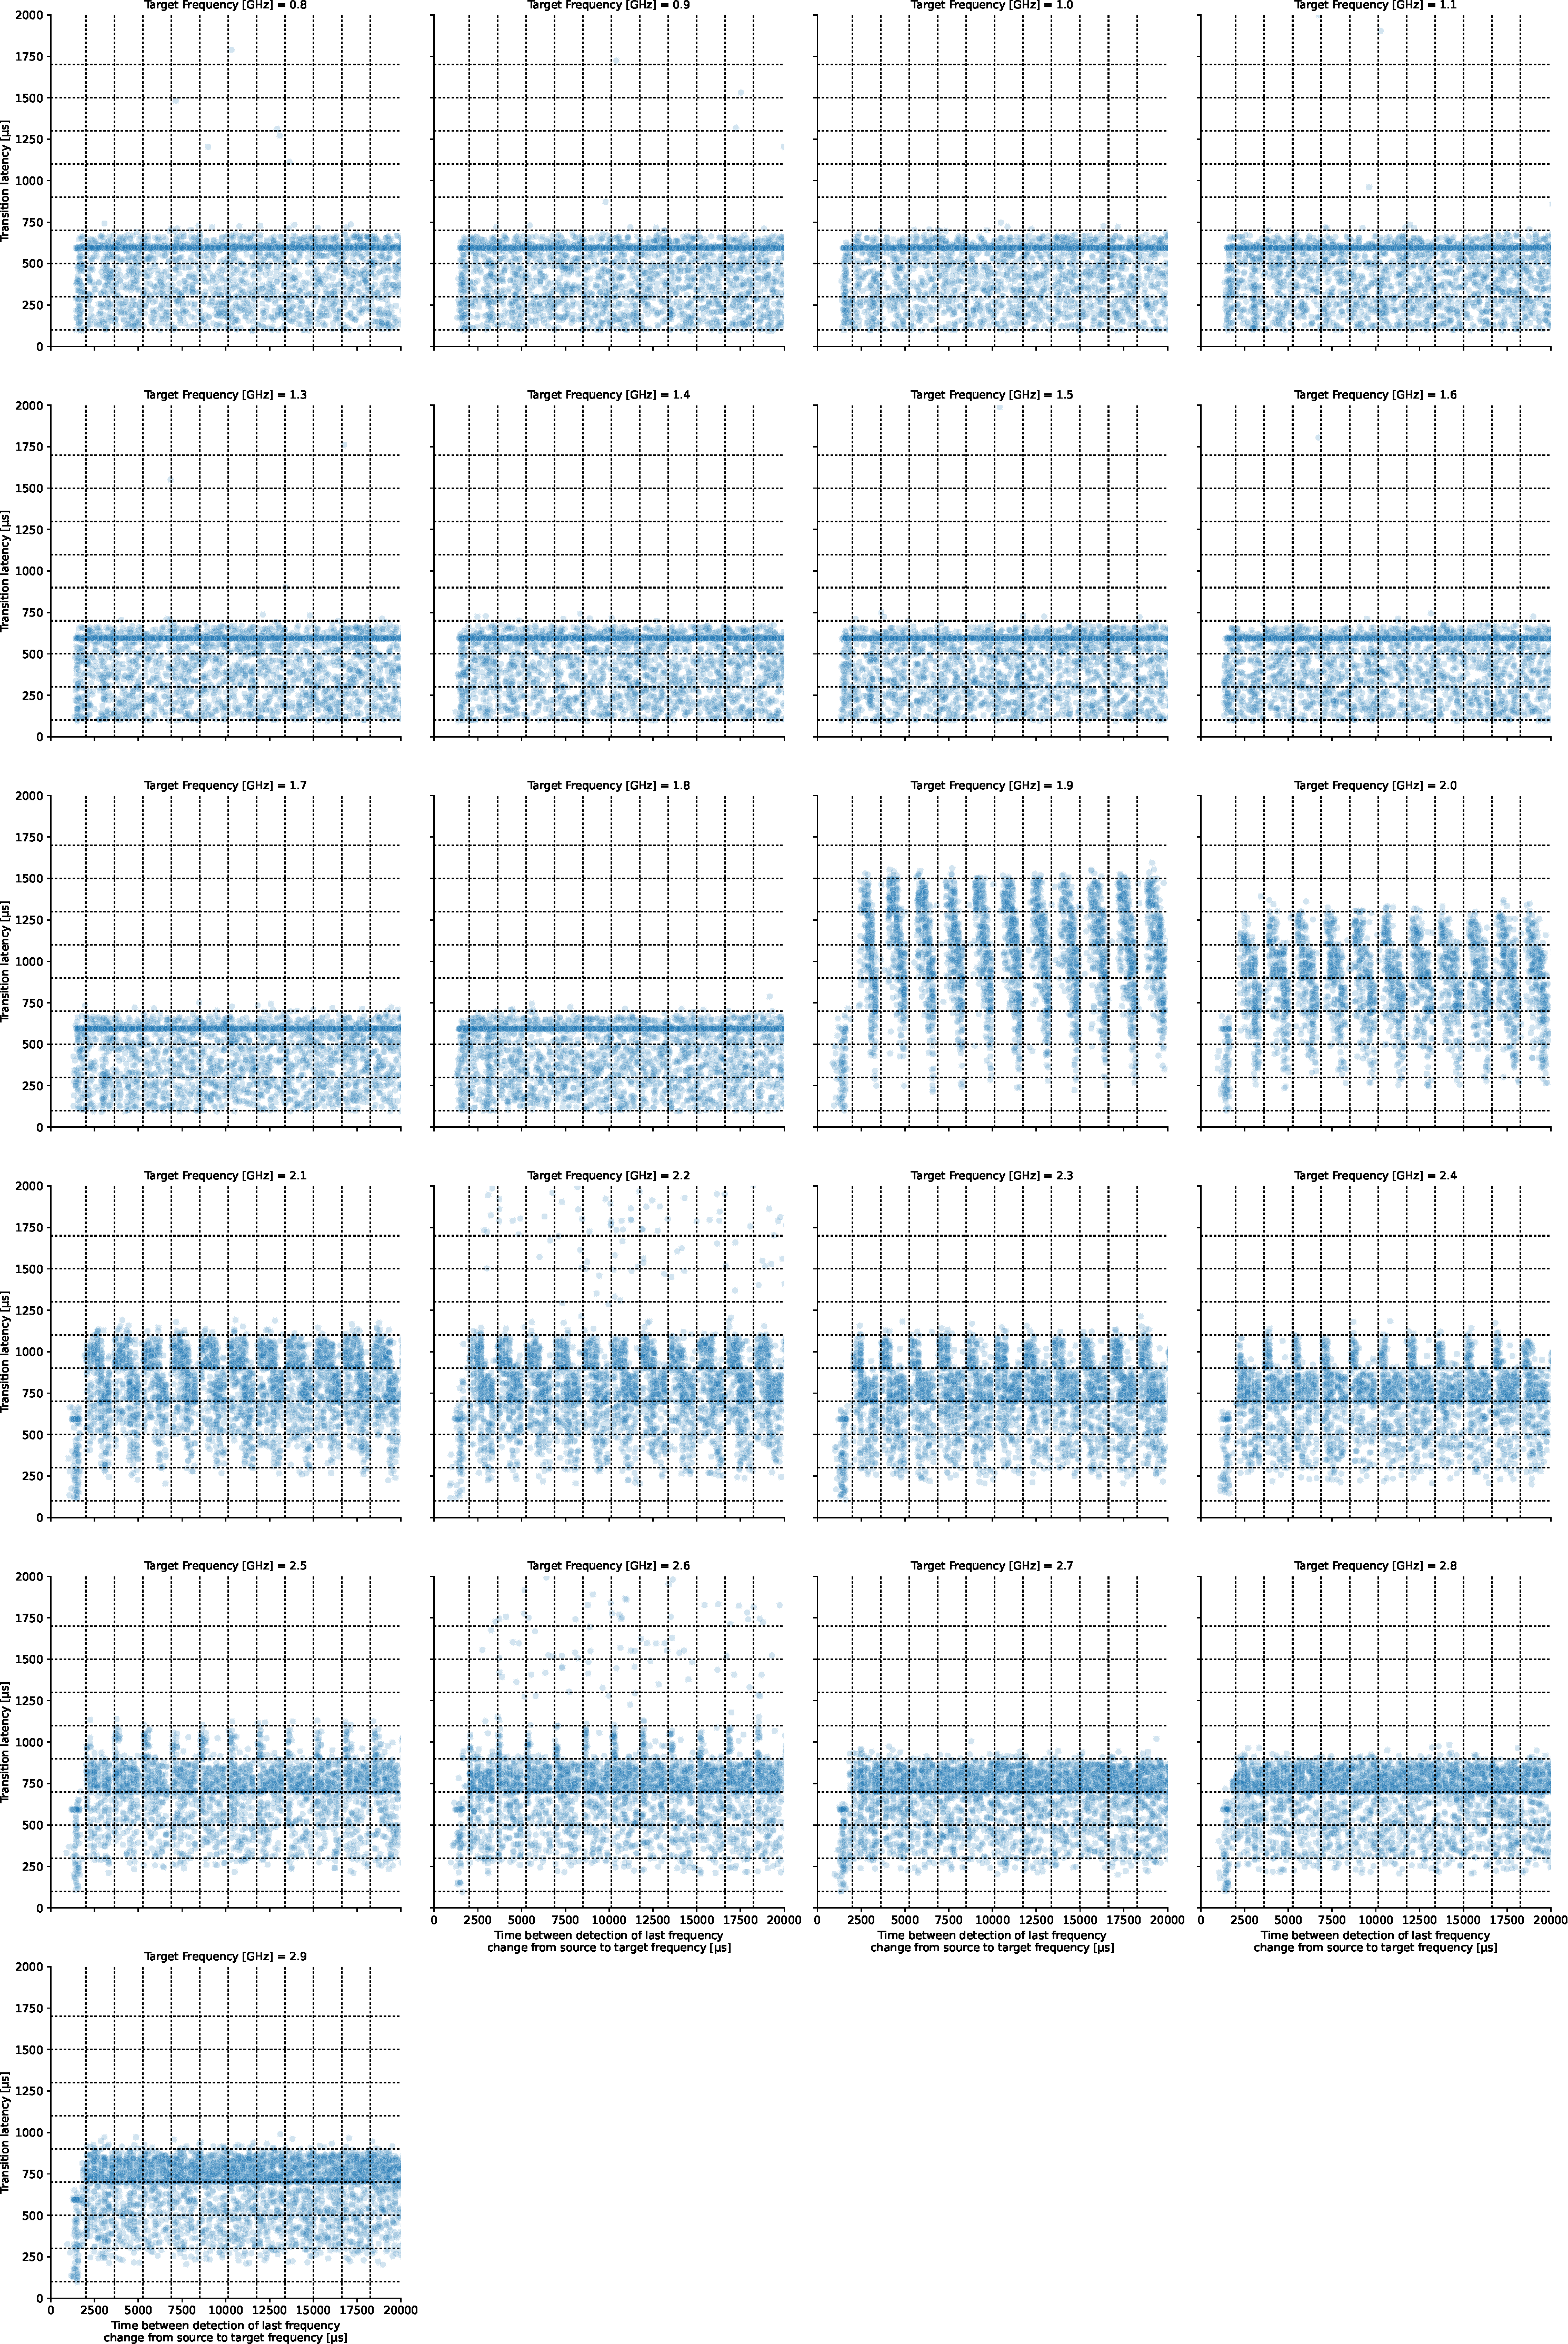
\includegraphics[width=\columnwidth]{fig/ftalat_scatter_wait_transition_latency_hati_source_1.2.pdf}
    \caption{Dependance of the time between the detection events of transitions from \SI{1.2}{\GHz} to \SI{0.8}{}, \SI{0.9}{}, ..., \SI{2.9}{\GHz}. For better lines for bins of size \SI{1625}{\us} and \SI{200}{\us} have been included for the x and y-axis respectively.}
\end{figure}
\begin{figure}[]
    \centering
    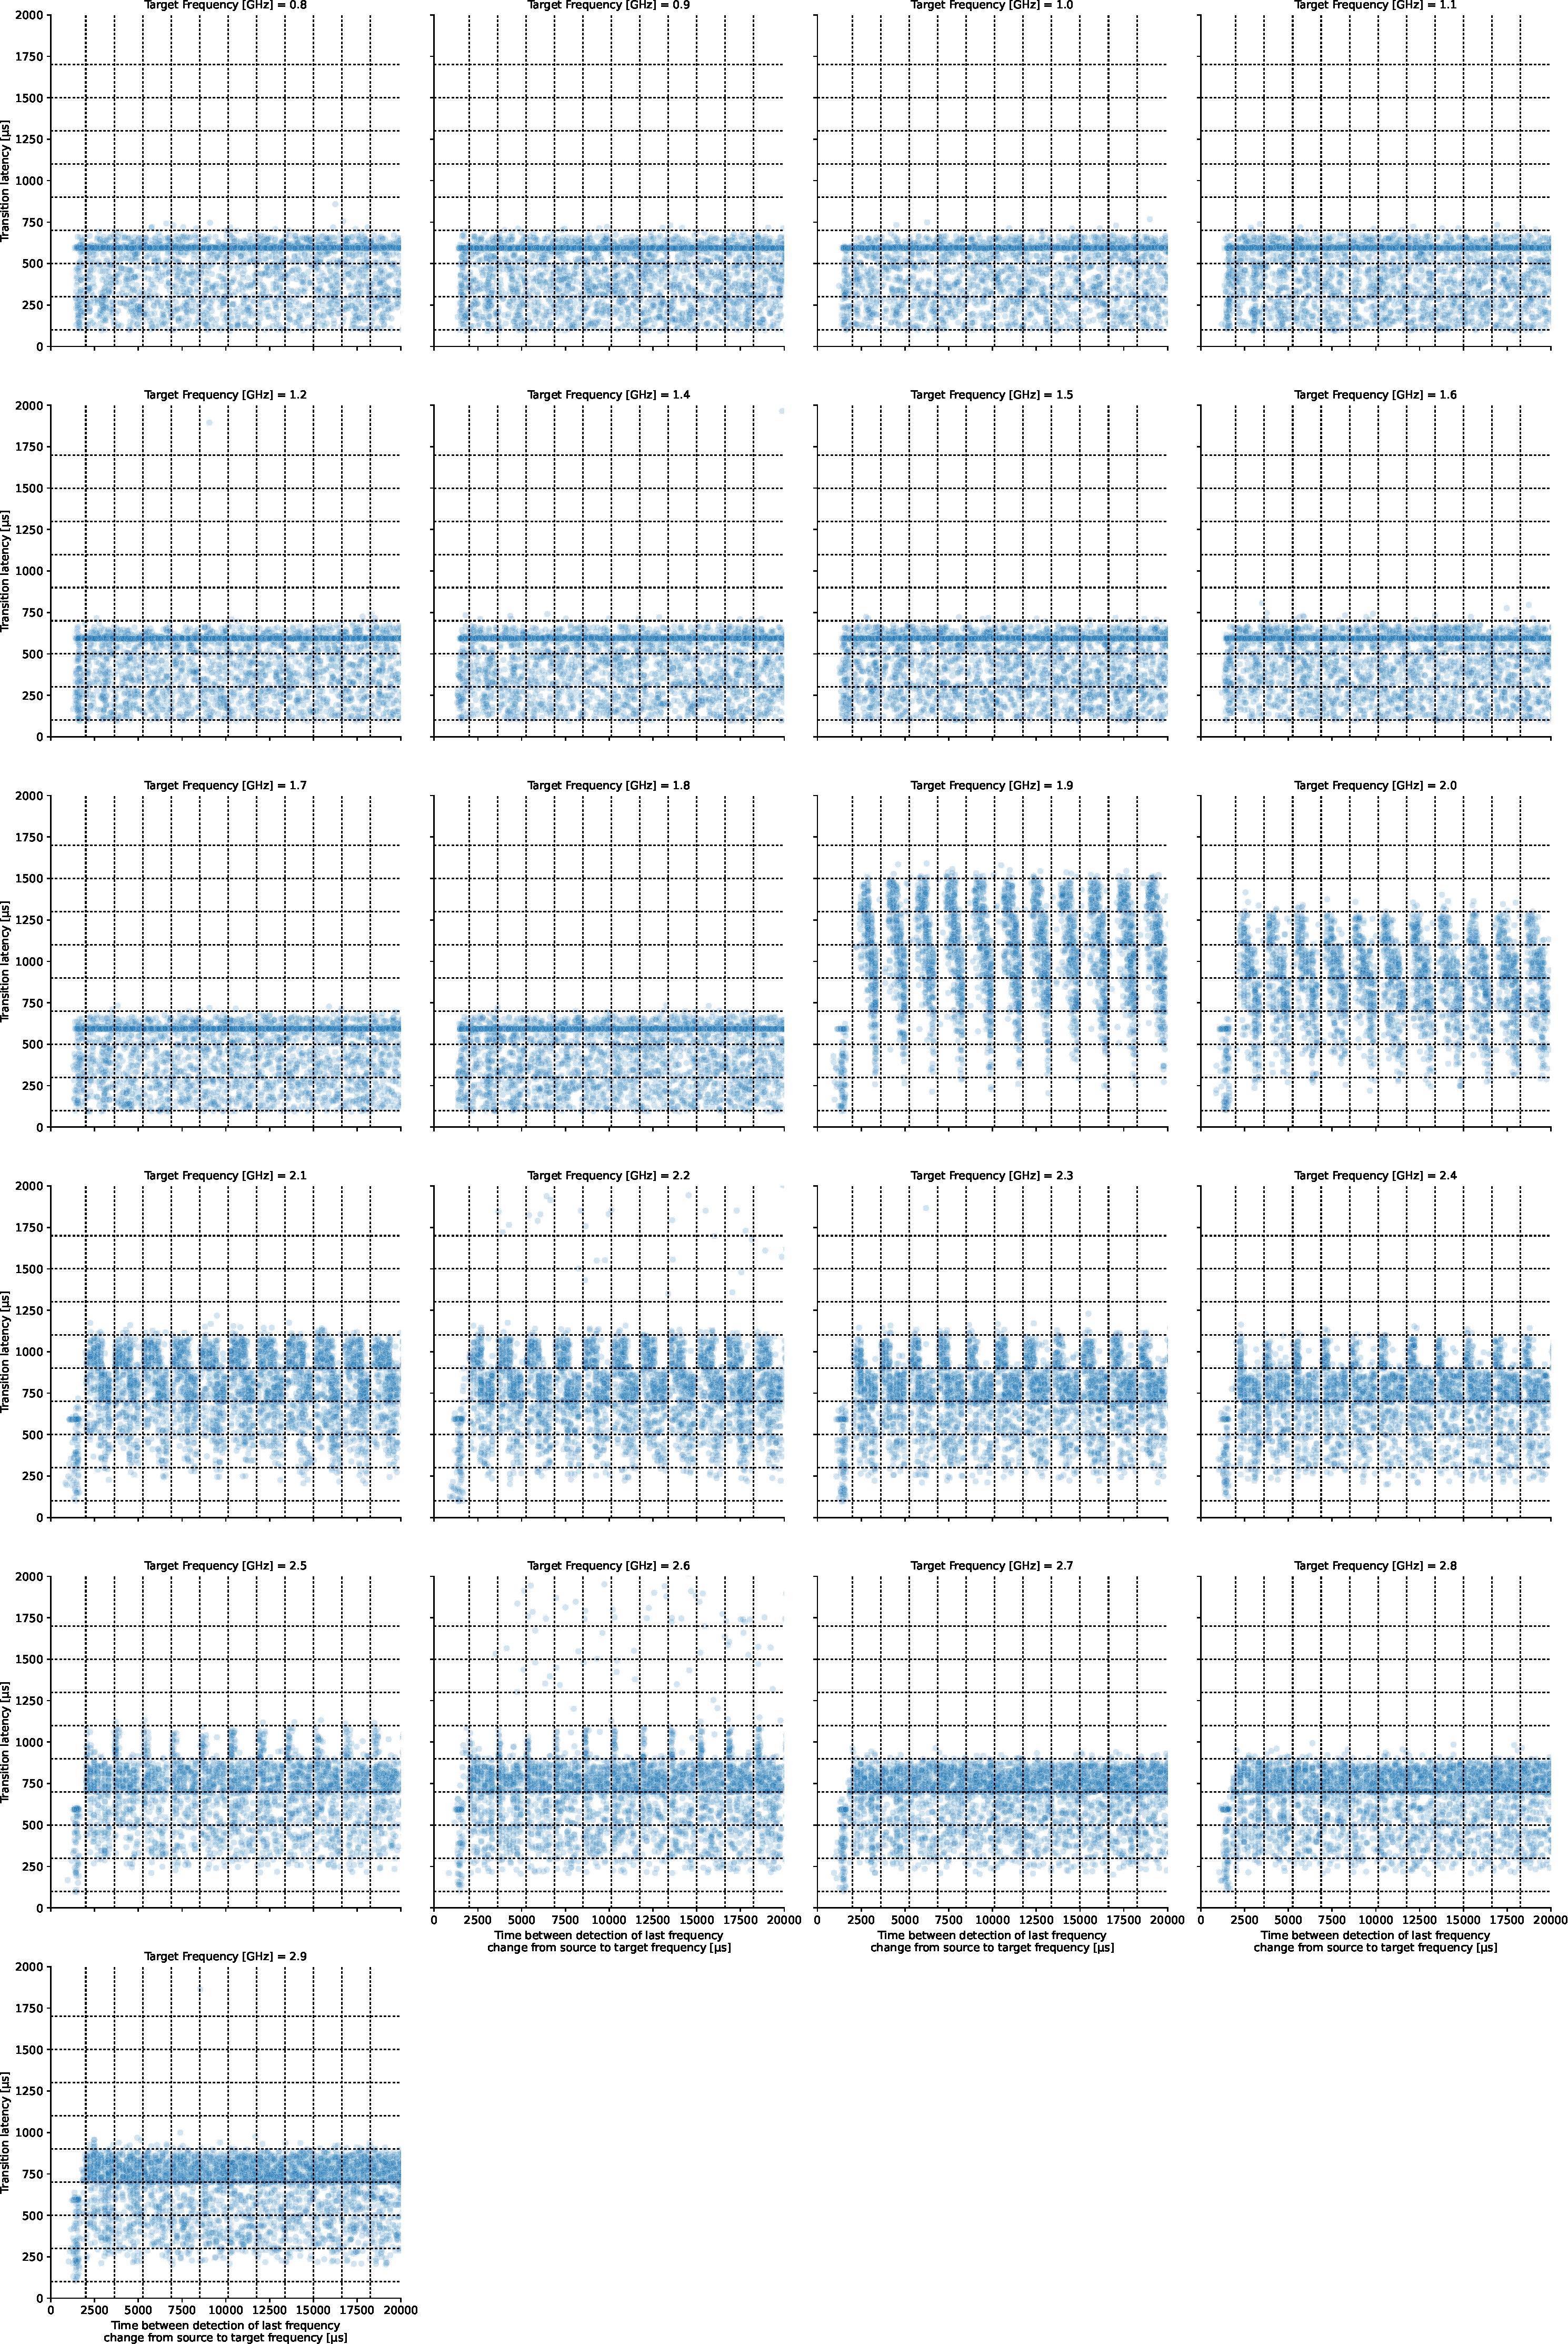
\includegraphics[width=\columnwidth]{fig/ftalat_scatter_wait_transition_latency_hati_source_1.3.pdf}
    \caption{Dependance of the time between the detection events of transitions from \SI{1.3}{\GHz} to \SI{0.8}{}, \SI{0.9}{}, ..., \SI{2.9}{\GHz}. For better lines for bins of size \SI{1625}{\us} and \SI{200}{\us} have been included for the x and y-axis respectively.}
\end{figure}
\begin{figure}[]
    \centering
    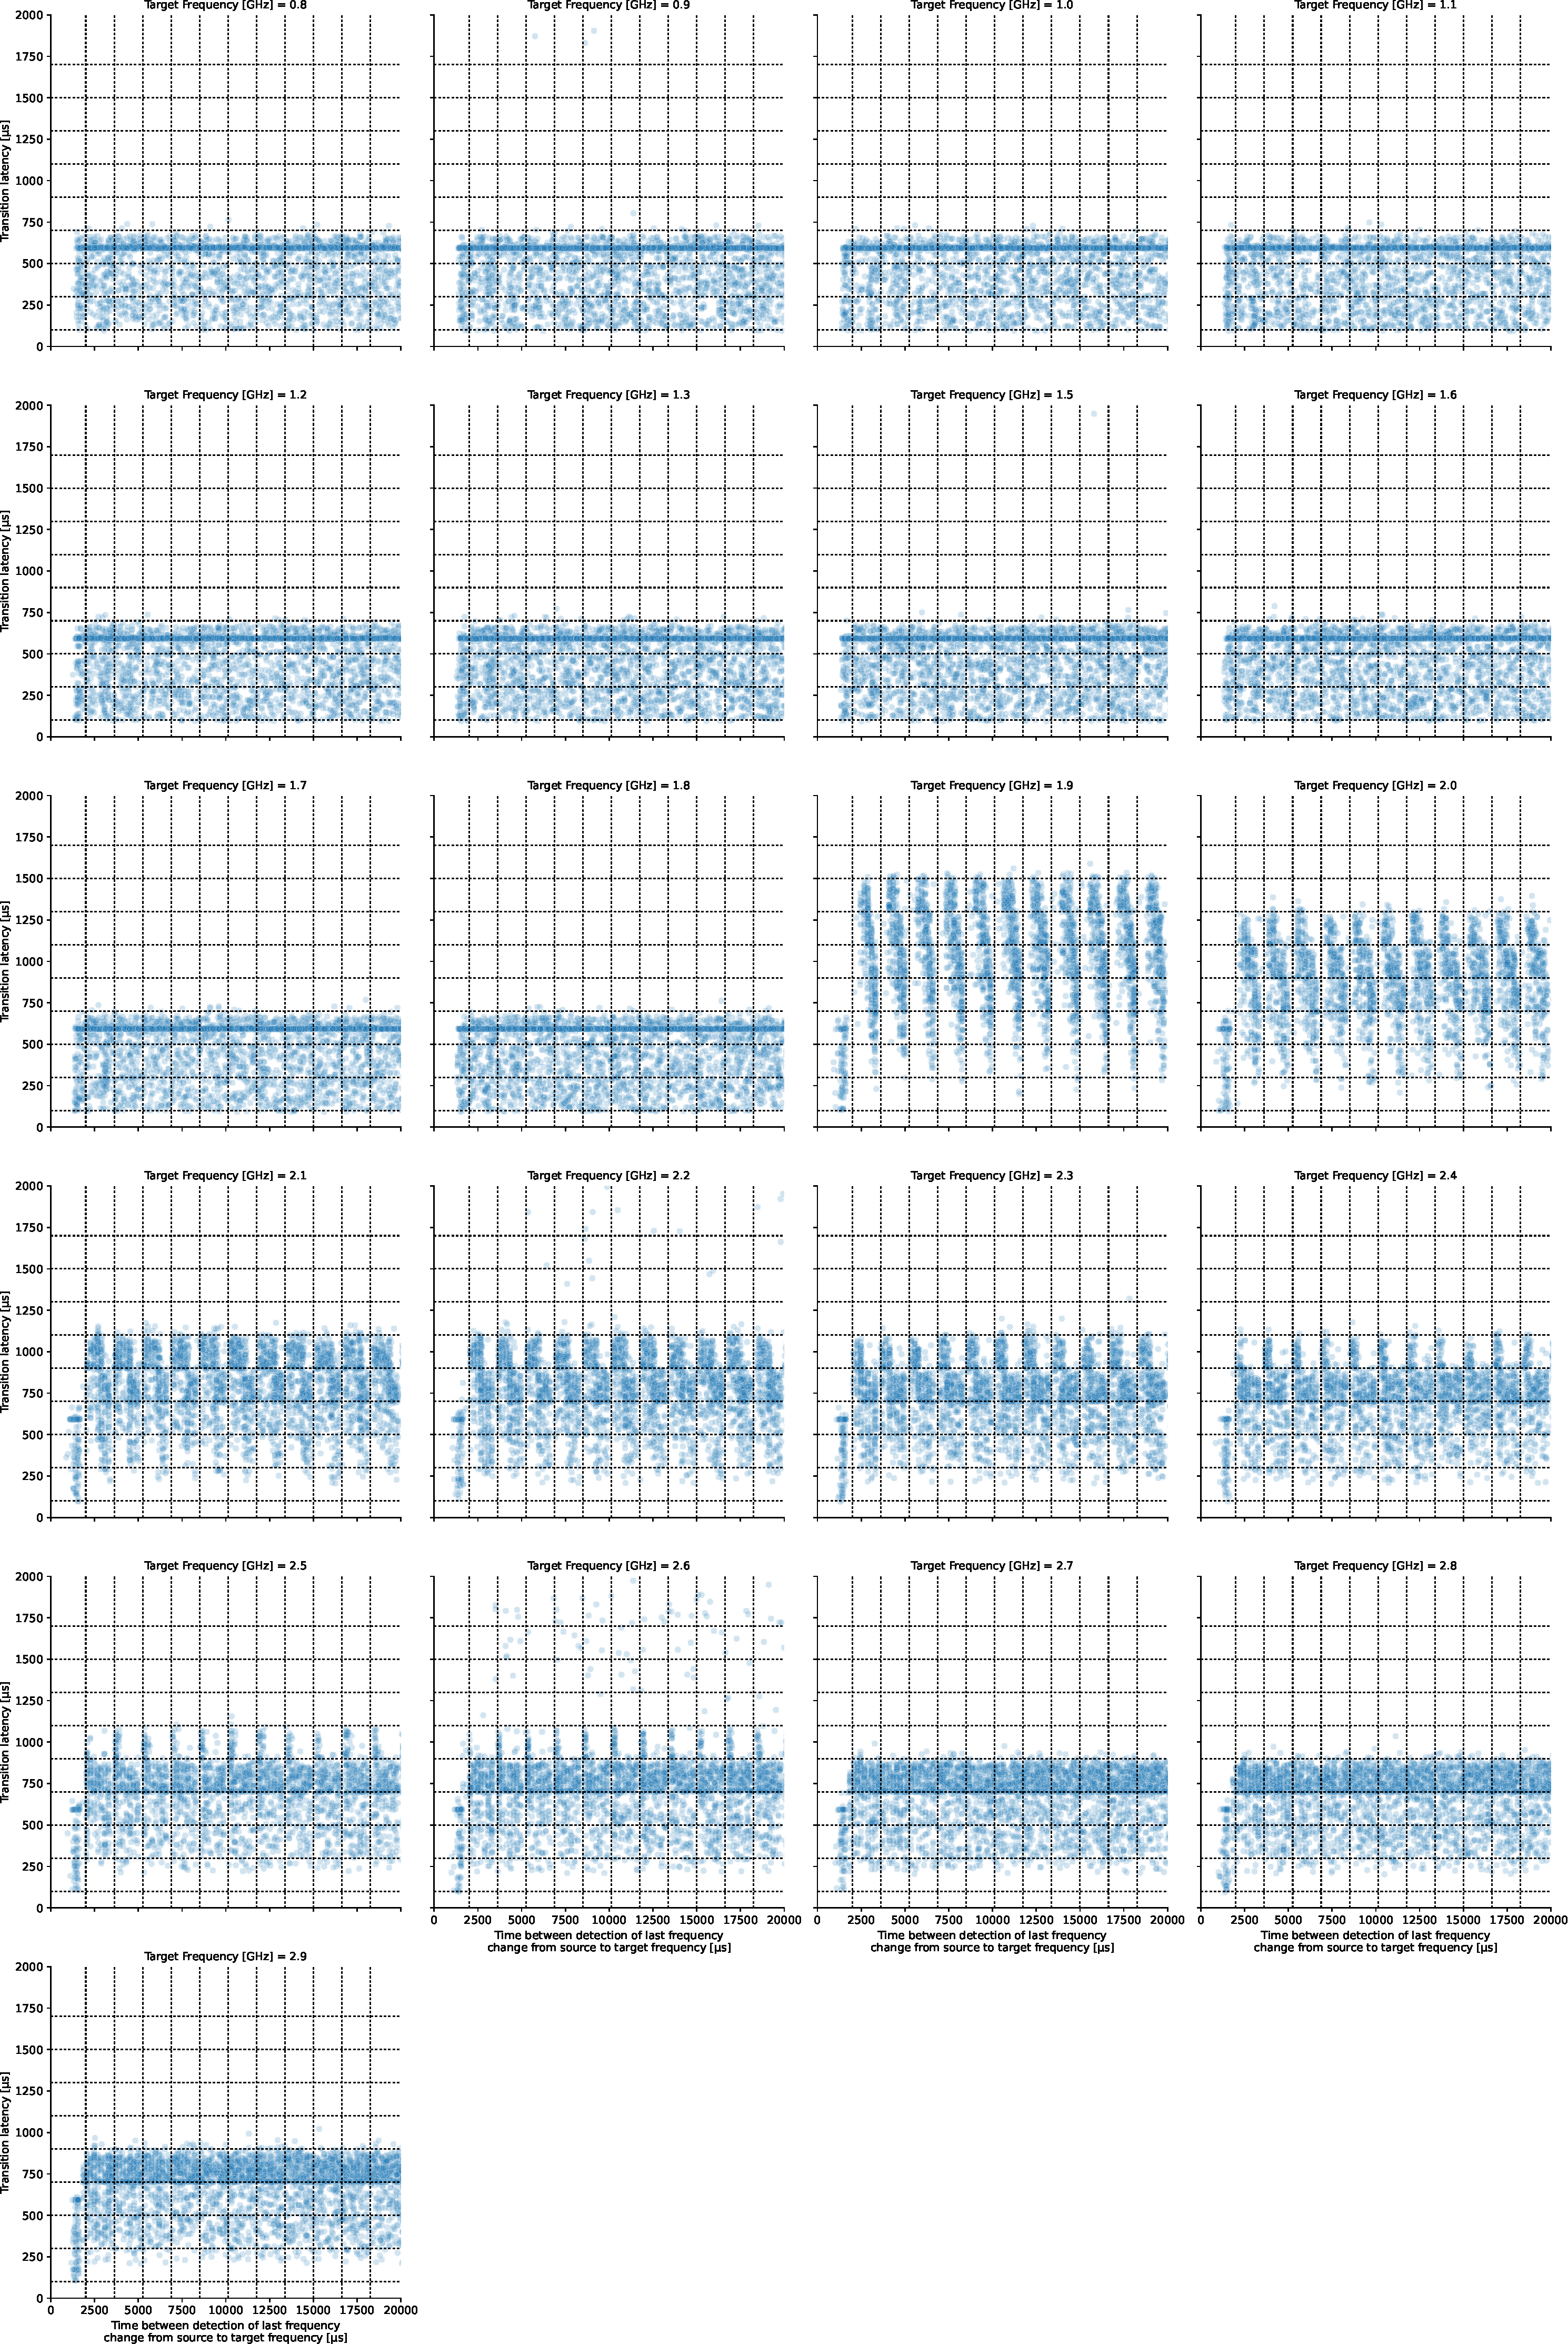
\includegraphics[width=\columnwidth]{fig/ftalat_scatter_wait_transition_latency_hati_source_1.4.pdf}
    \caption{Dependance of the time between the detection events of transitions from \SI{1.4}{\GHz} to \SI{0.8}{}, \SI{0.9}{}, ..., \SI{2.9}{\GHz}. For better lines for bins of size \SI{1625}{\us} and \SI{200}{\us} have been included for the x and y-axis respectively.}
\end{figure}
\begin{figure}[]
    \centering
    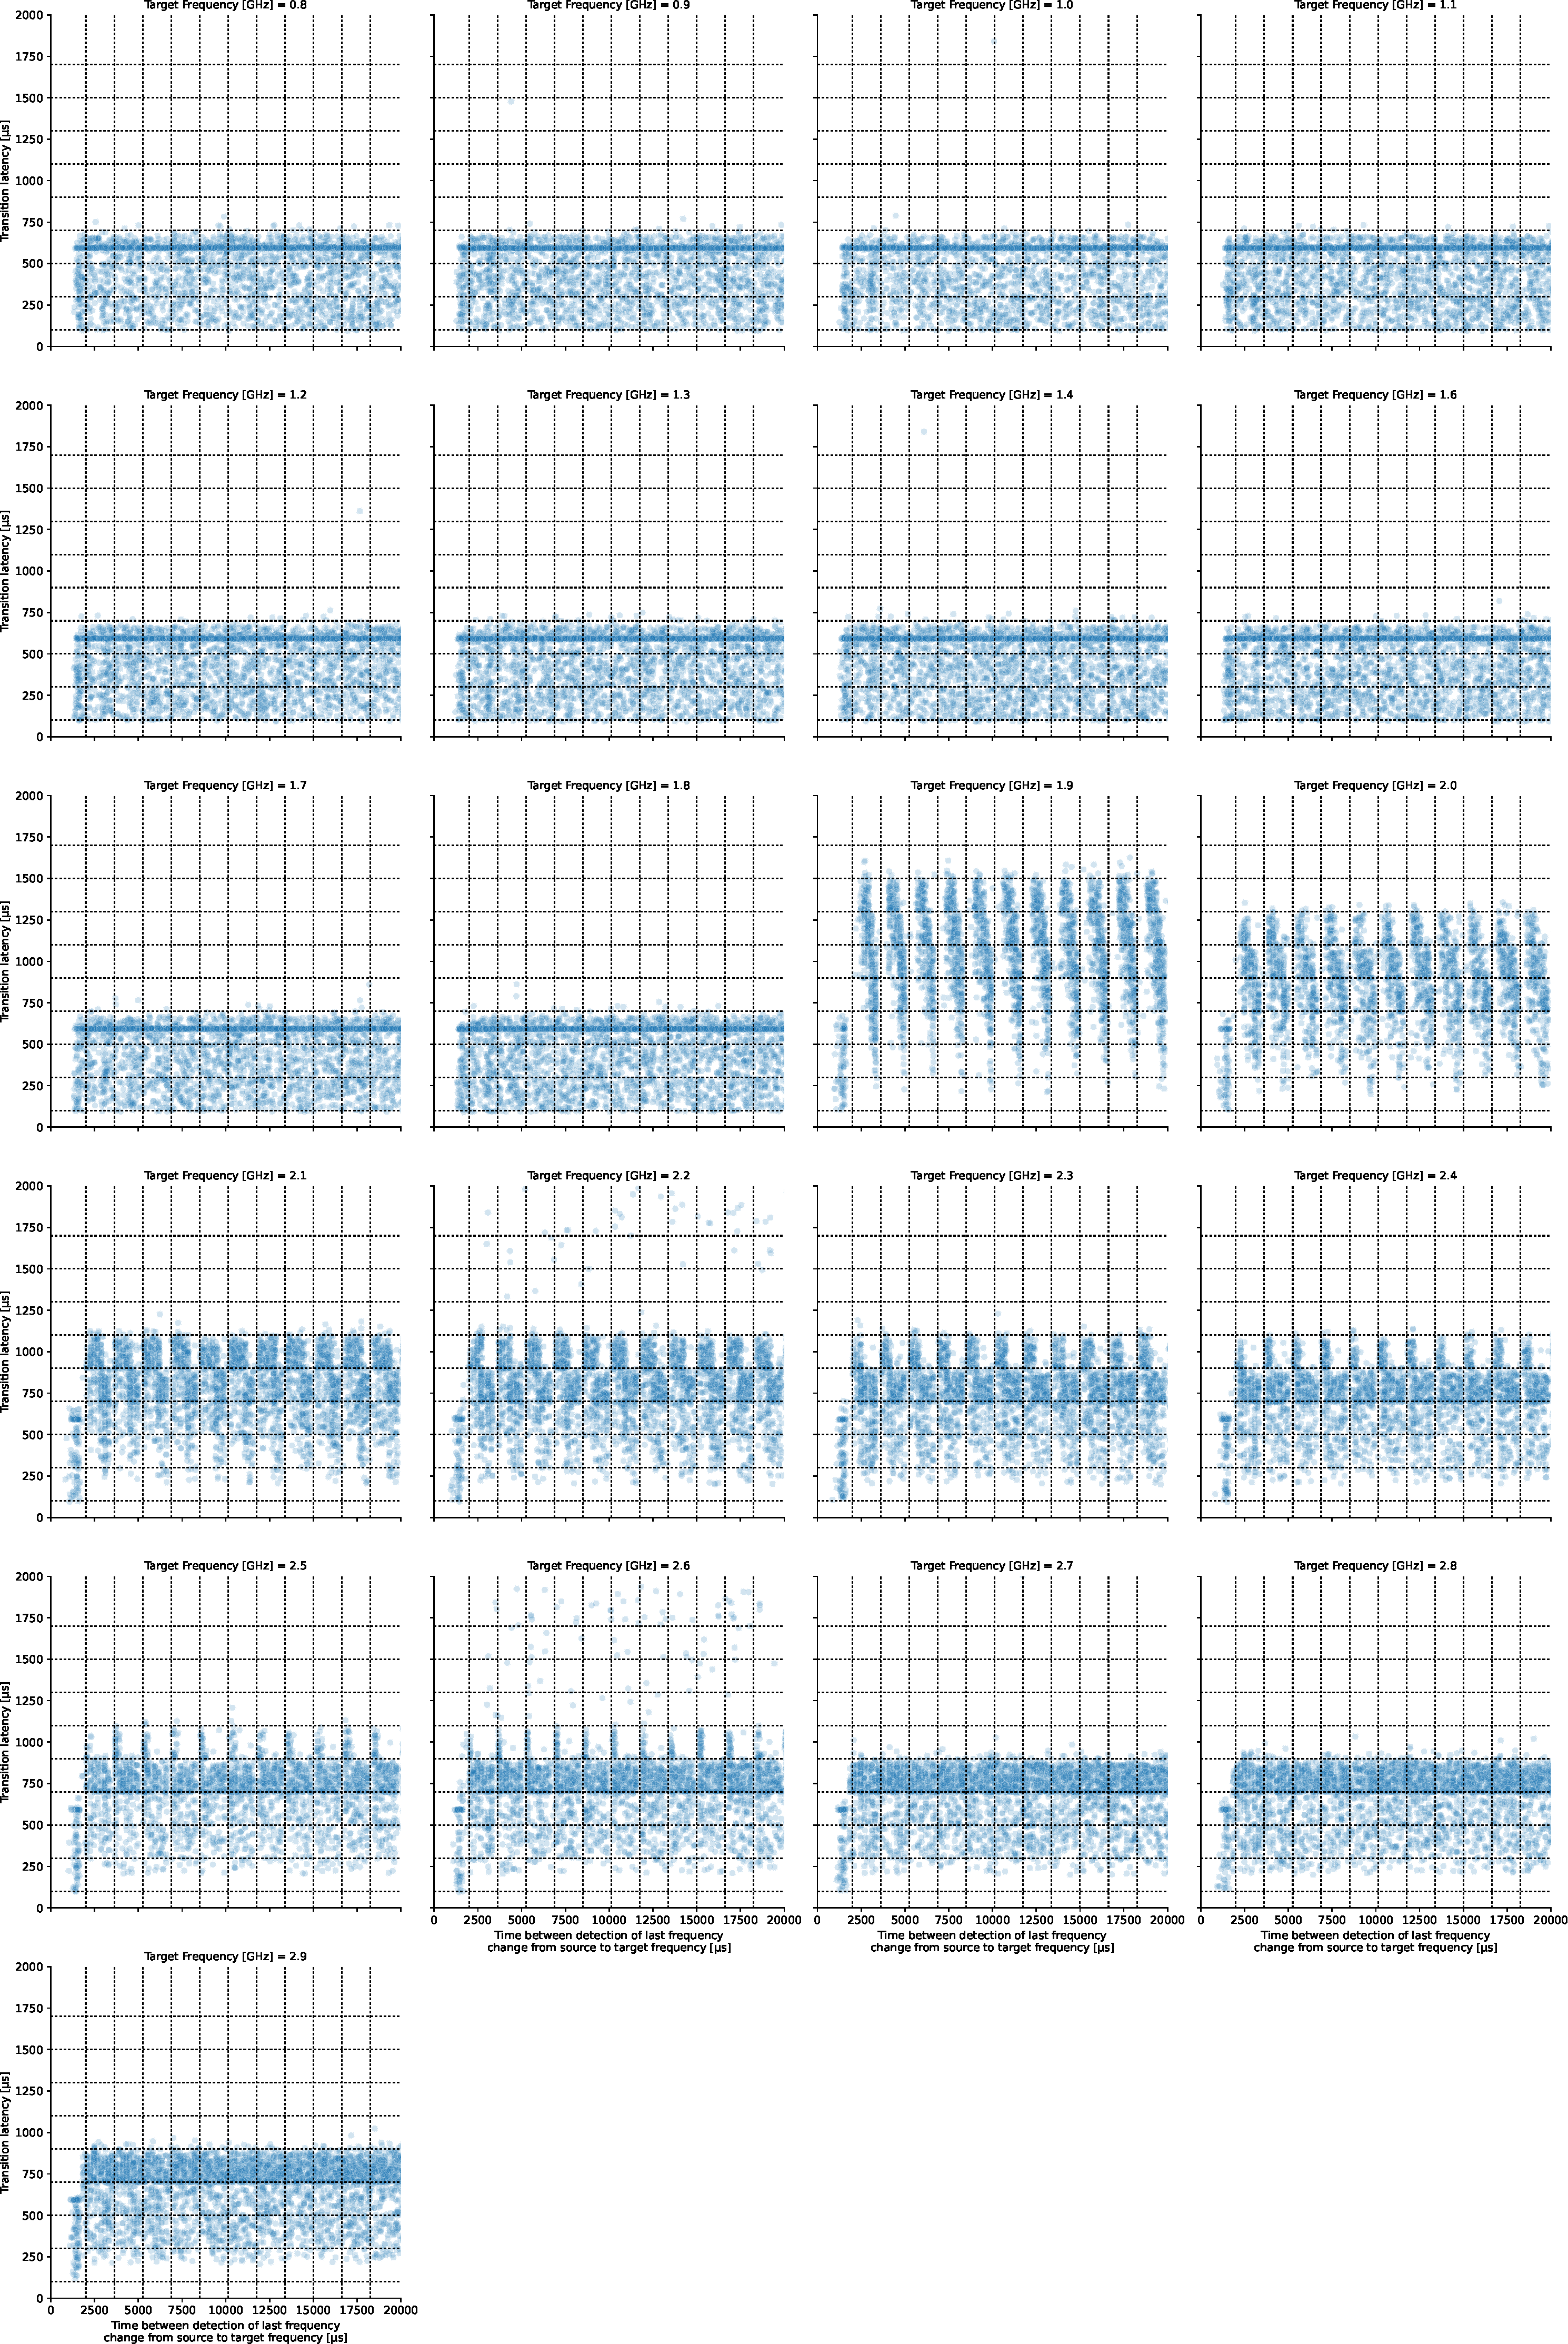
\includegraphics[width=\columnwidth]{fig/ftalat_scatter_wait_transition_latency_hati_source_1.5.pdf}
    \caption{Dependance of the time between the detection events of transitions from \SI{1.5}{\GHz} to \SI{0.8}{}, \SI{0.9}{}, ..., \SI{2.9}{\GHz}. For better lines for bins of size \SI{1625}{\us} and \SI{200}{\us} have been included for the x and y-axis respectively.}
\end{figure}
\begin{figure}[]
    \centering
    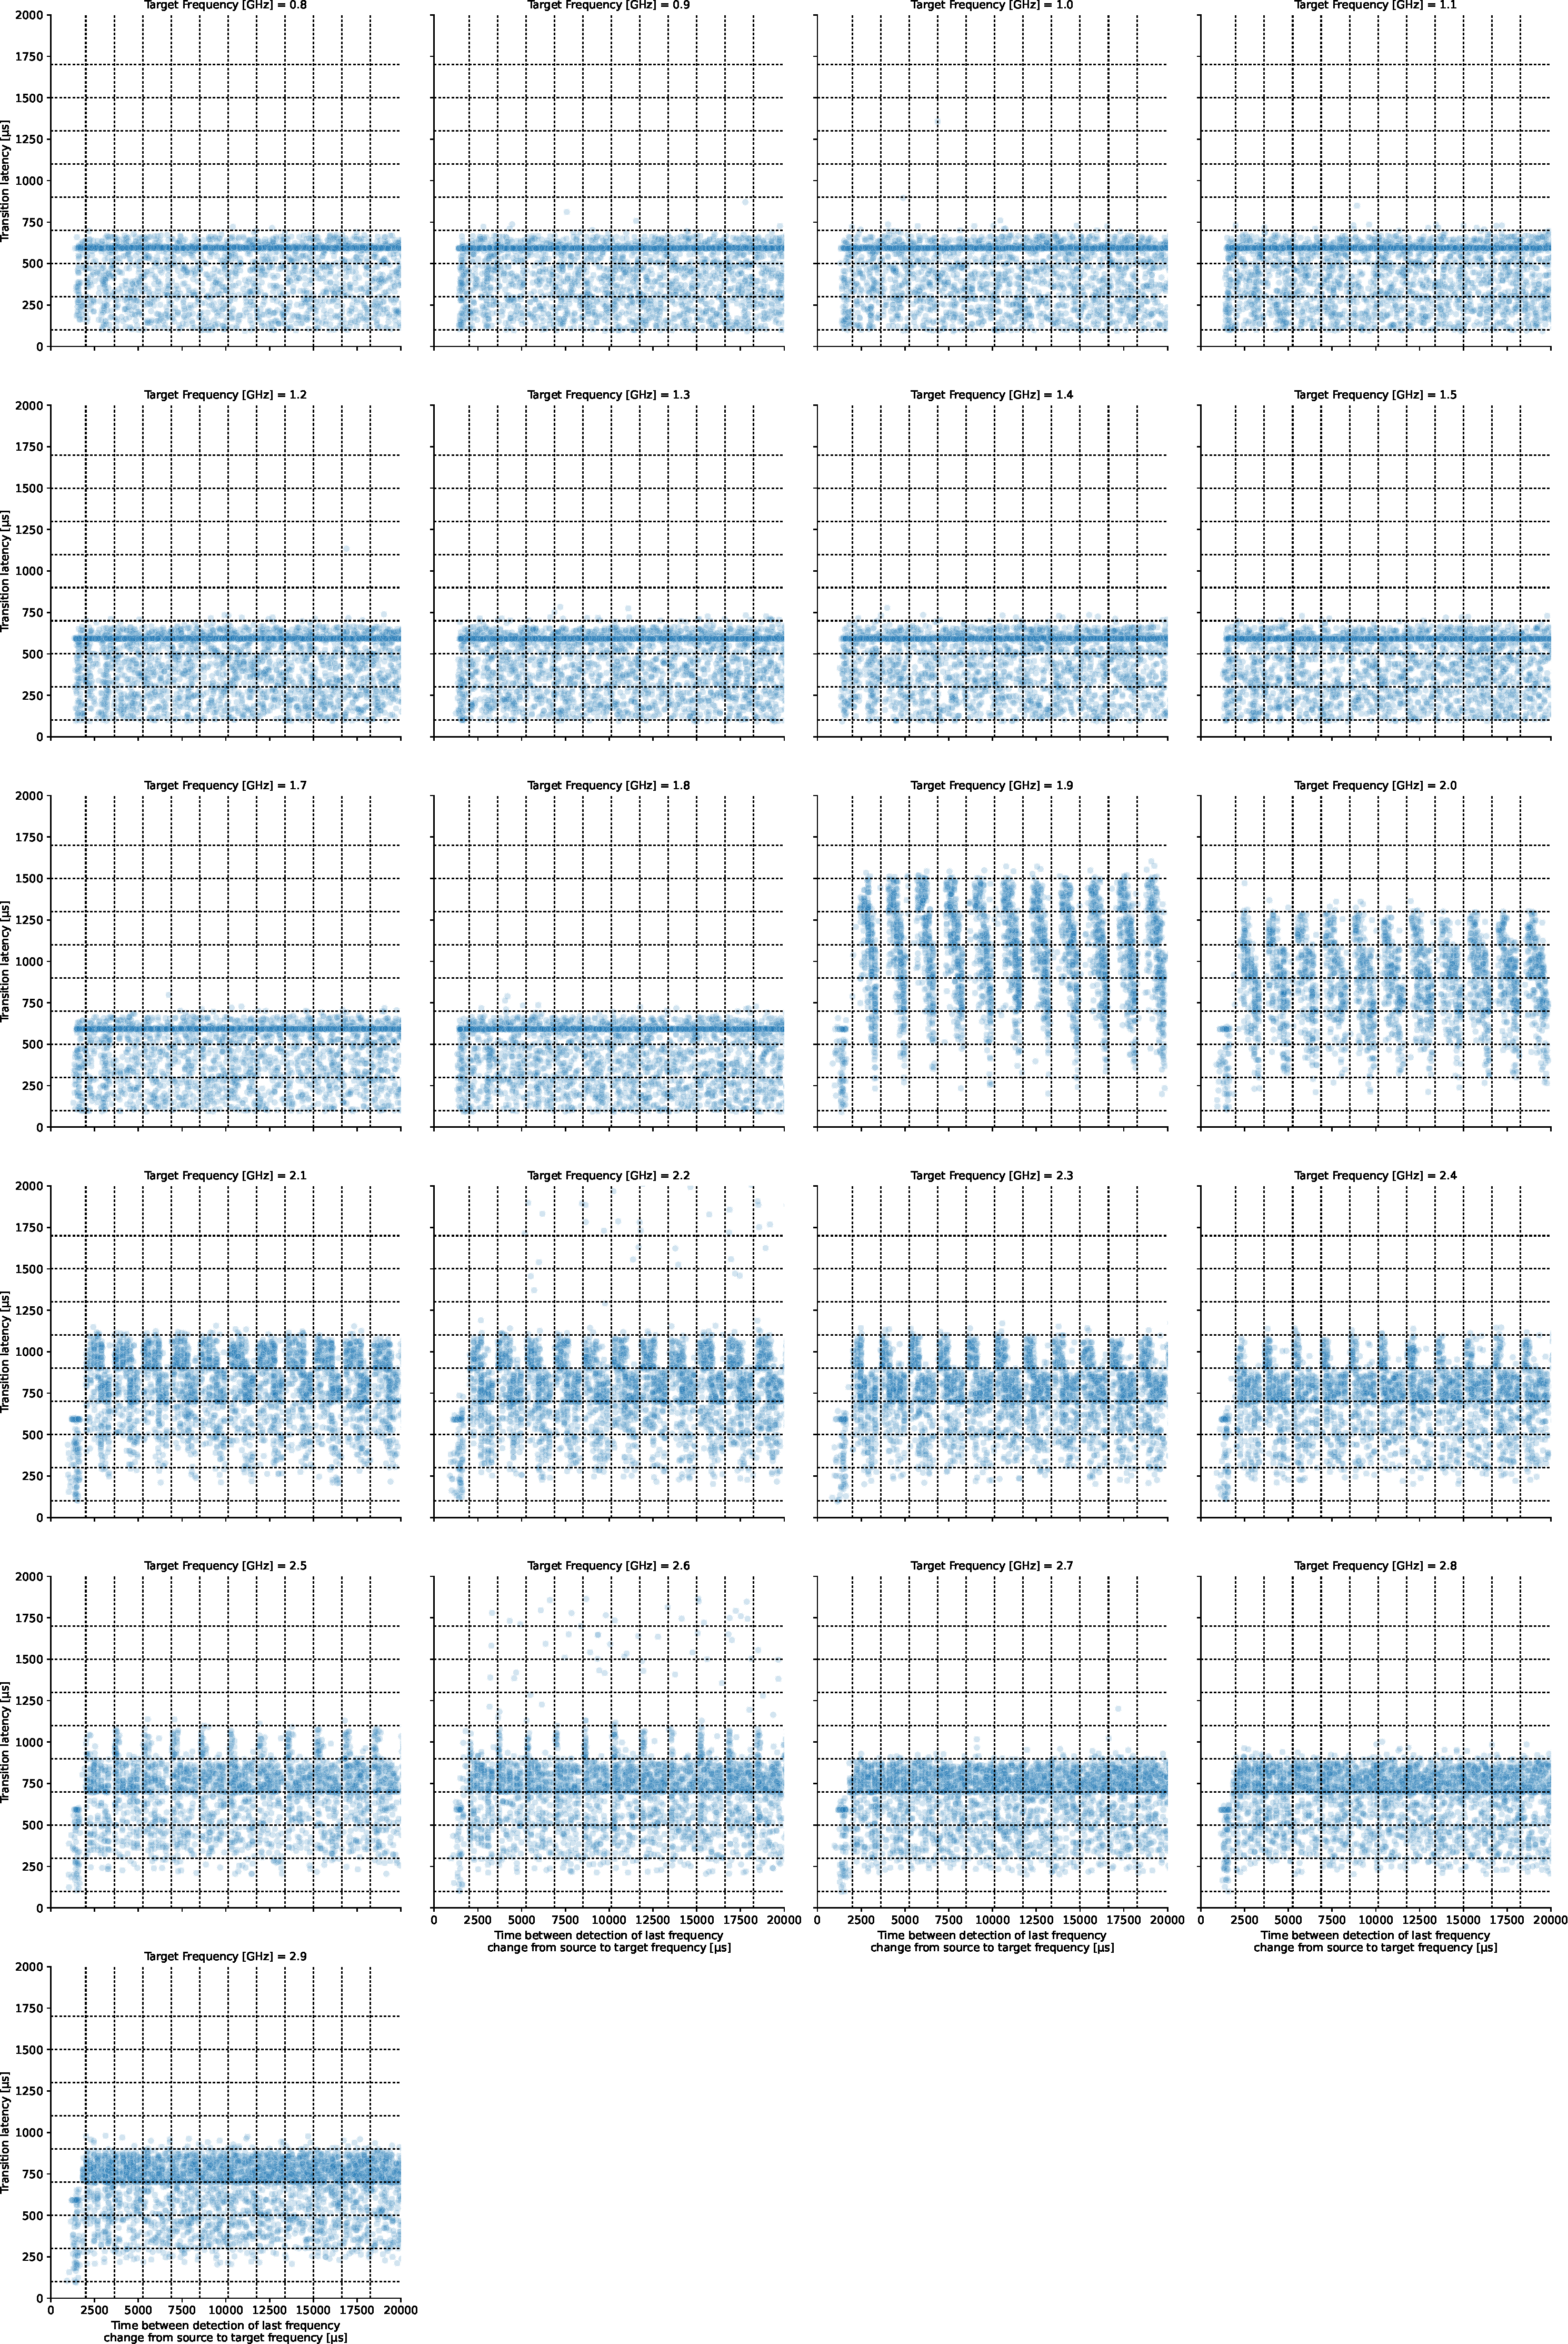
\includegraphics[width=\columnwidth]{fig/ftalat_scatter_wait_transition_latency_hati_source_1.6.pdf}
    \caption{Dependance of the time between the detection events of transitions from \SI{1.6}{\GHz} to \SI{0.8}{}, \SI{0.9}{}, ..., \SI{2.9}{\GHz}. For better lines for bins of size \SI{1625}{\us} and \SI{200}{\us} have been included for the x and y-axis respectively.}
\end{figure}
\begin{figure}[]
    \centering
    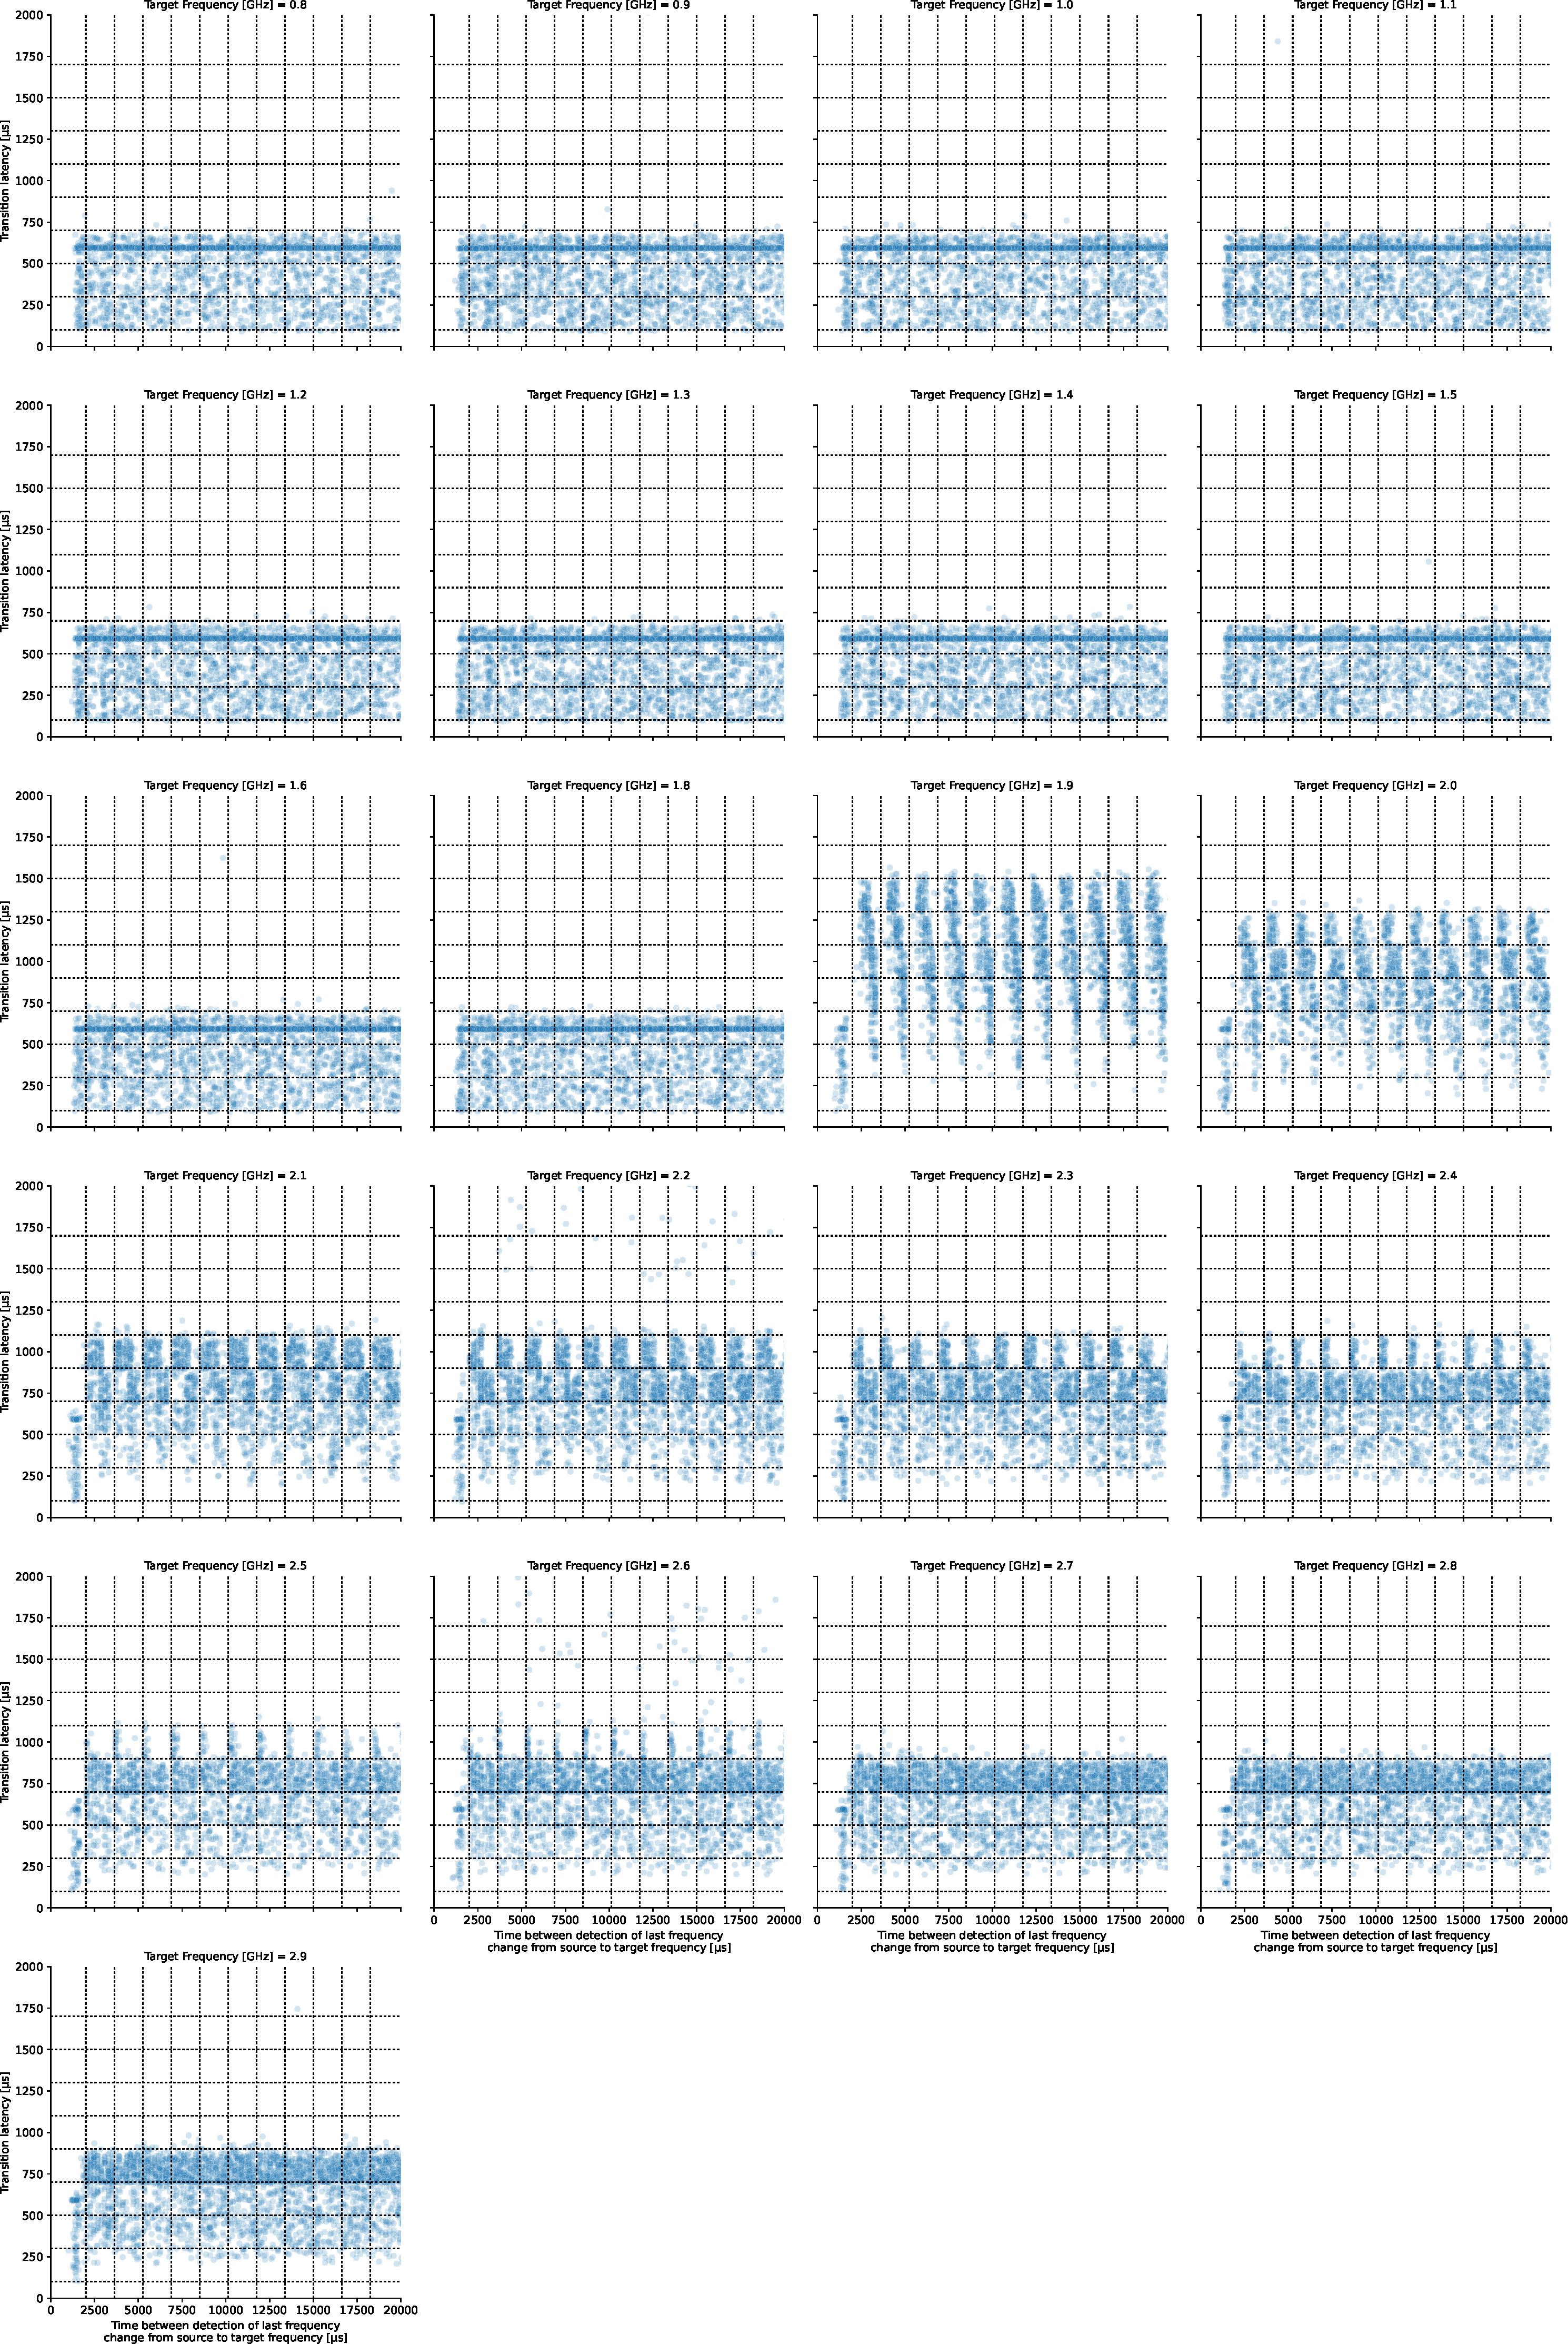
\includegraphics[width=\columnwidth]{fig/ftalat_scatter_wait_transition_latency_hati_source_1.7.pdf}
    \caption{Dependance of the time between the detection events of transitions from \SI{1.7}{\GHz} to \SI{0.8}{}, \SI{0.9}{}, ..., \SI{2.9}{\GHz}. For better lines for bins of size \SI{1625}{\us} and \SI{200}{\us} have been included for the x and y-axis respectively.}
\end{figure}
\begin{figure}[]
    \centering
    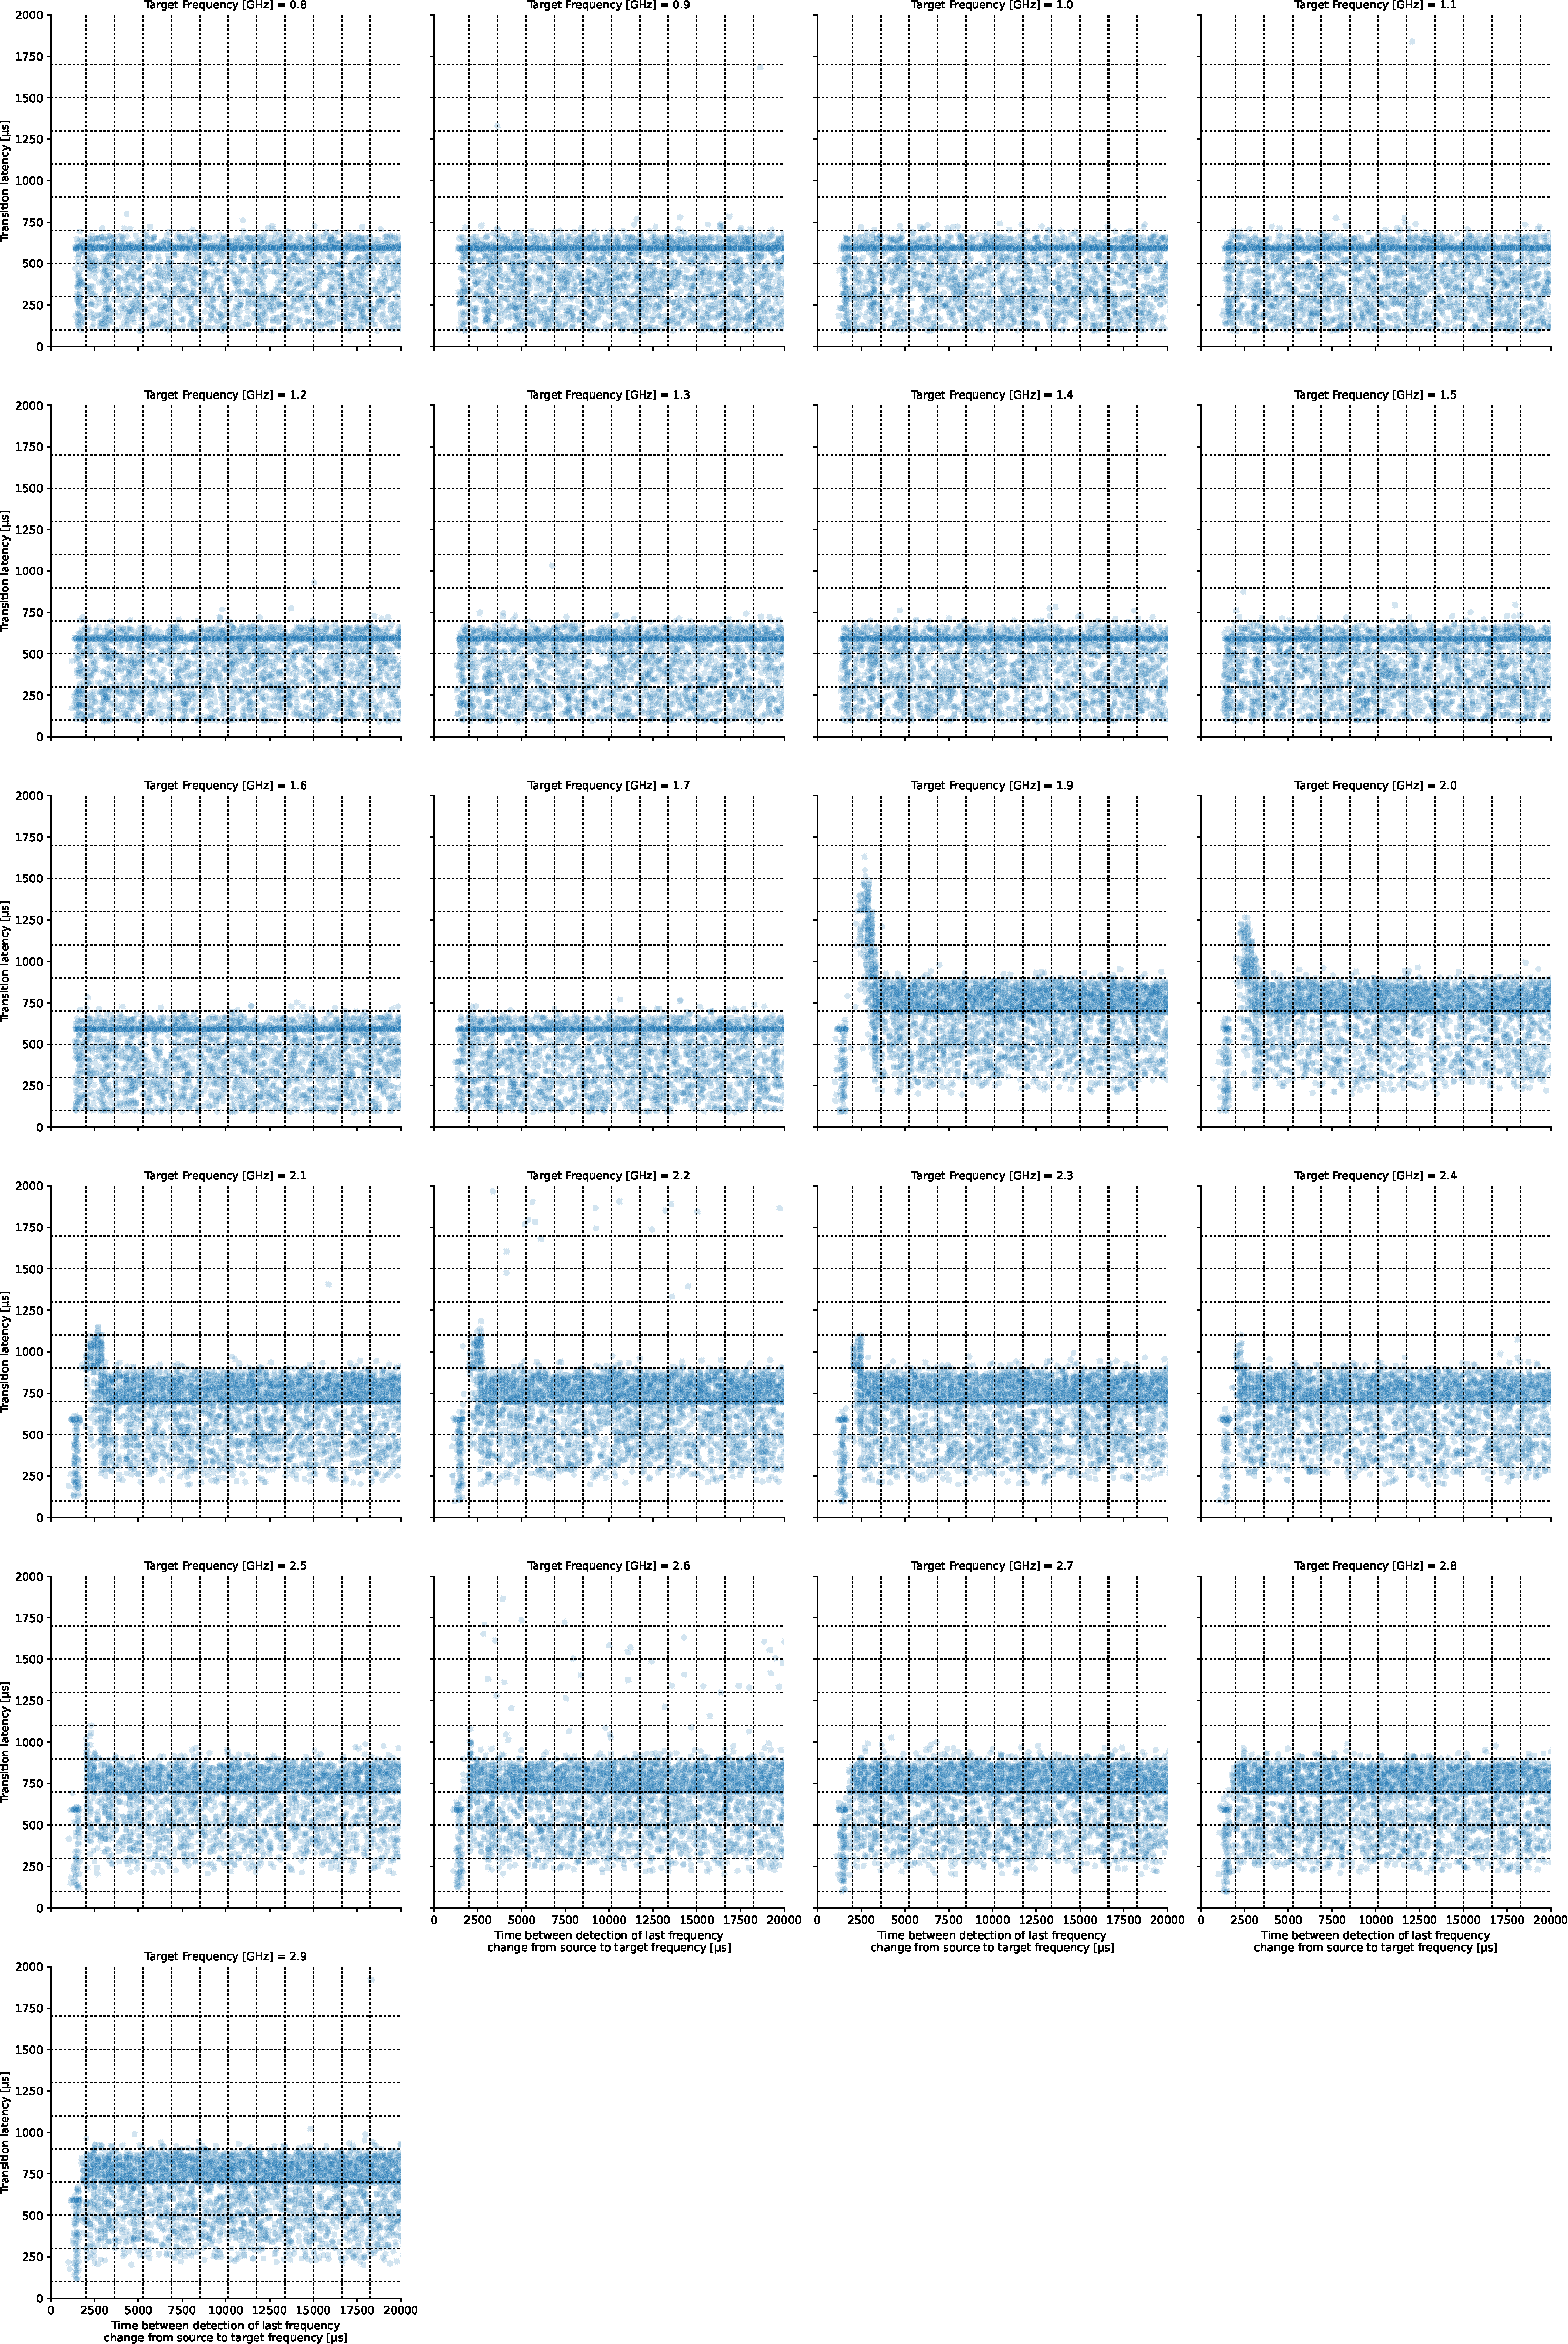
\includegraphics[width=\columnwidth]{fig/ftalat_scatter_wait_transition_latency_hati_source_1.8.pdf}
    \caption{Dependance of the time between the detection events of transitions from \SI{1.8}{\GHz} to \SI{0.8}{}, \SI{0.9}{}, ..., \SI{2.9}{\GHz}. For better lines for bins of size \SI{1625}{\us} and \SI{200}{\us} have been included for the x and y-axis respectively.}
\end{figure}
\begin{figure}[]
    \centering
    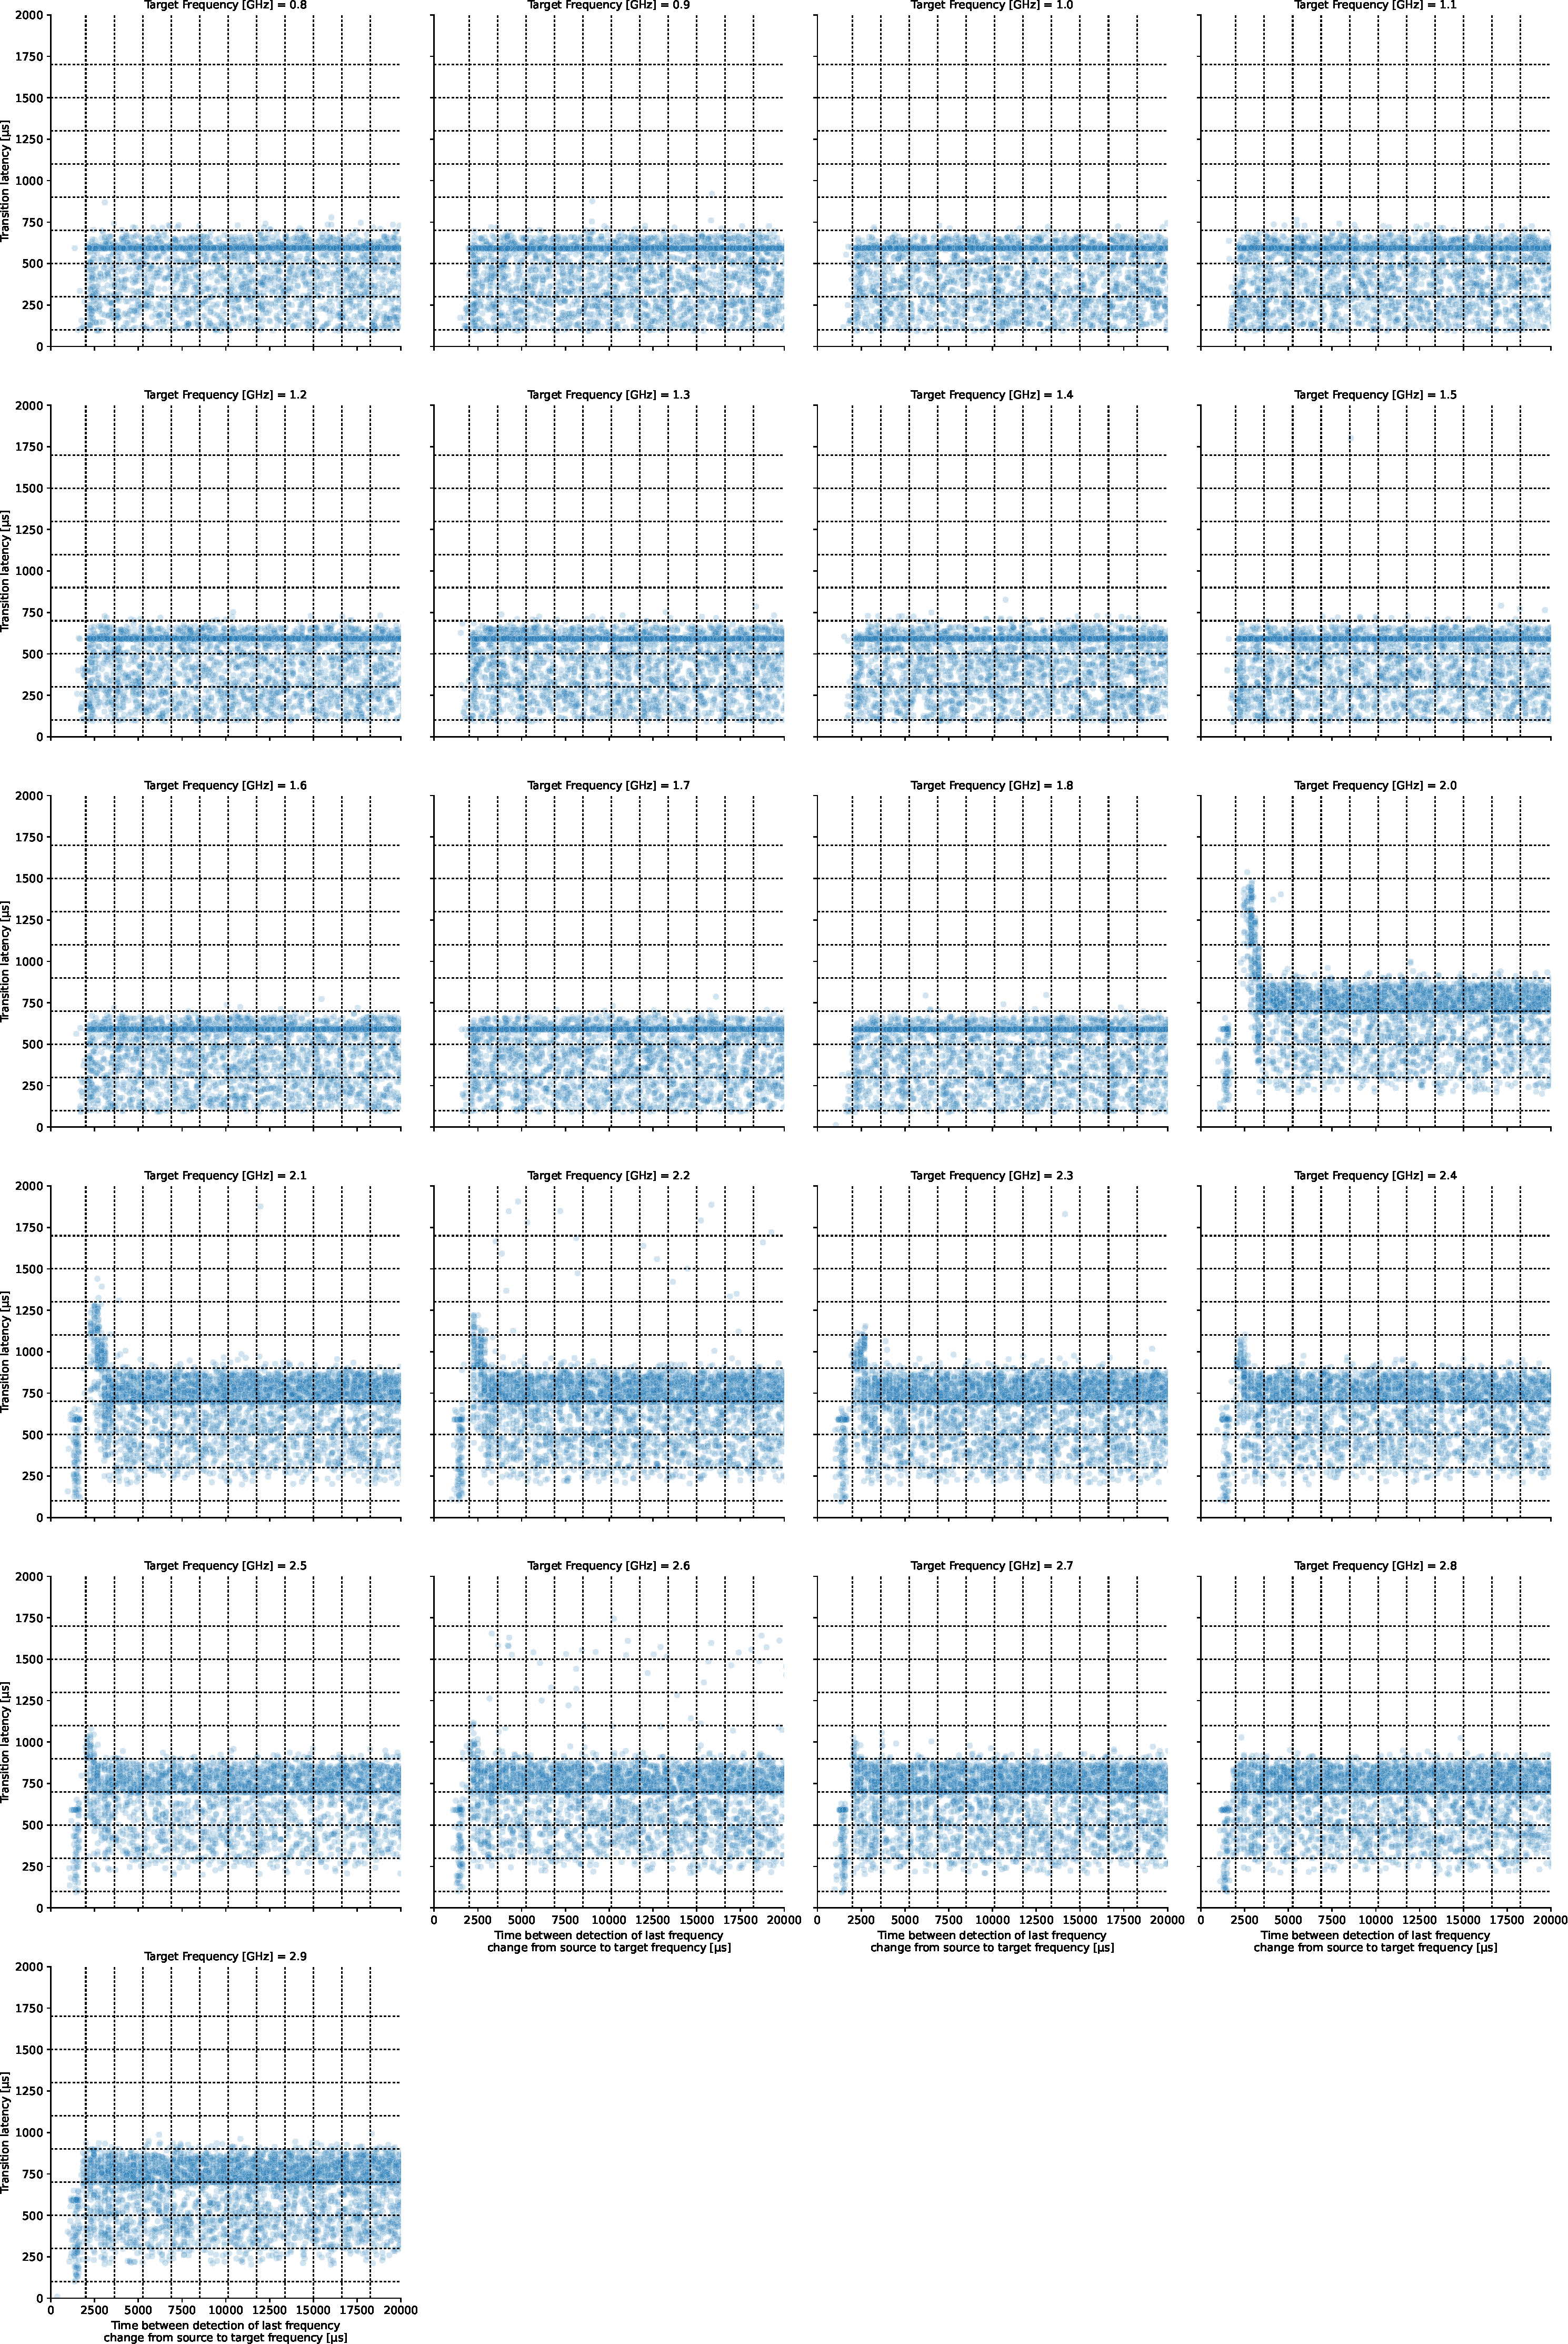
\includegraphics[width=\columnwidth]{fig/ftalat_scatter_wait_transition_latency_hati_source_1.9.pdf}
    \caption{Dependance of the time between the detection events of transitions from \SI{1.9}{\GHz} to \SI{0.8}{}, \SI{0.9}{}, ..., \SI{2.9}{\GHz}. For better lines for bins of size \SI{1625}{\us} and \SI{200}{\us} have been included for the x and y-axis respectively.}
\end{figure}
\begin{figure}[]
    \centering
    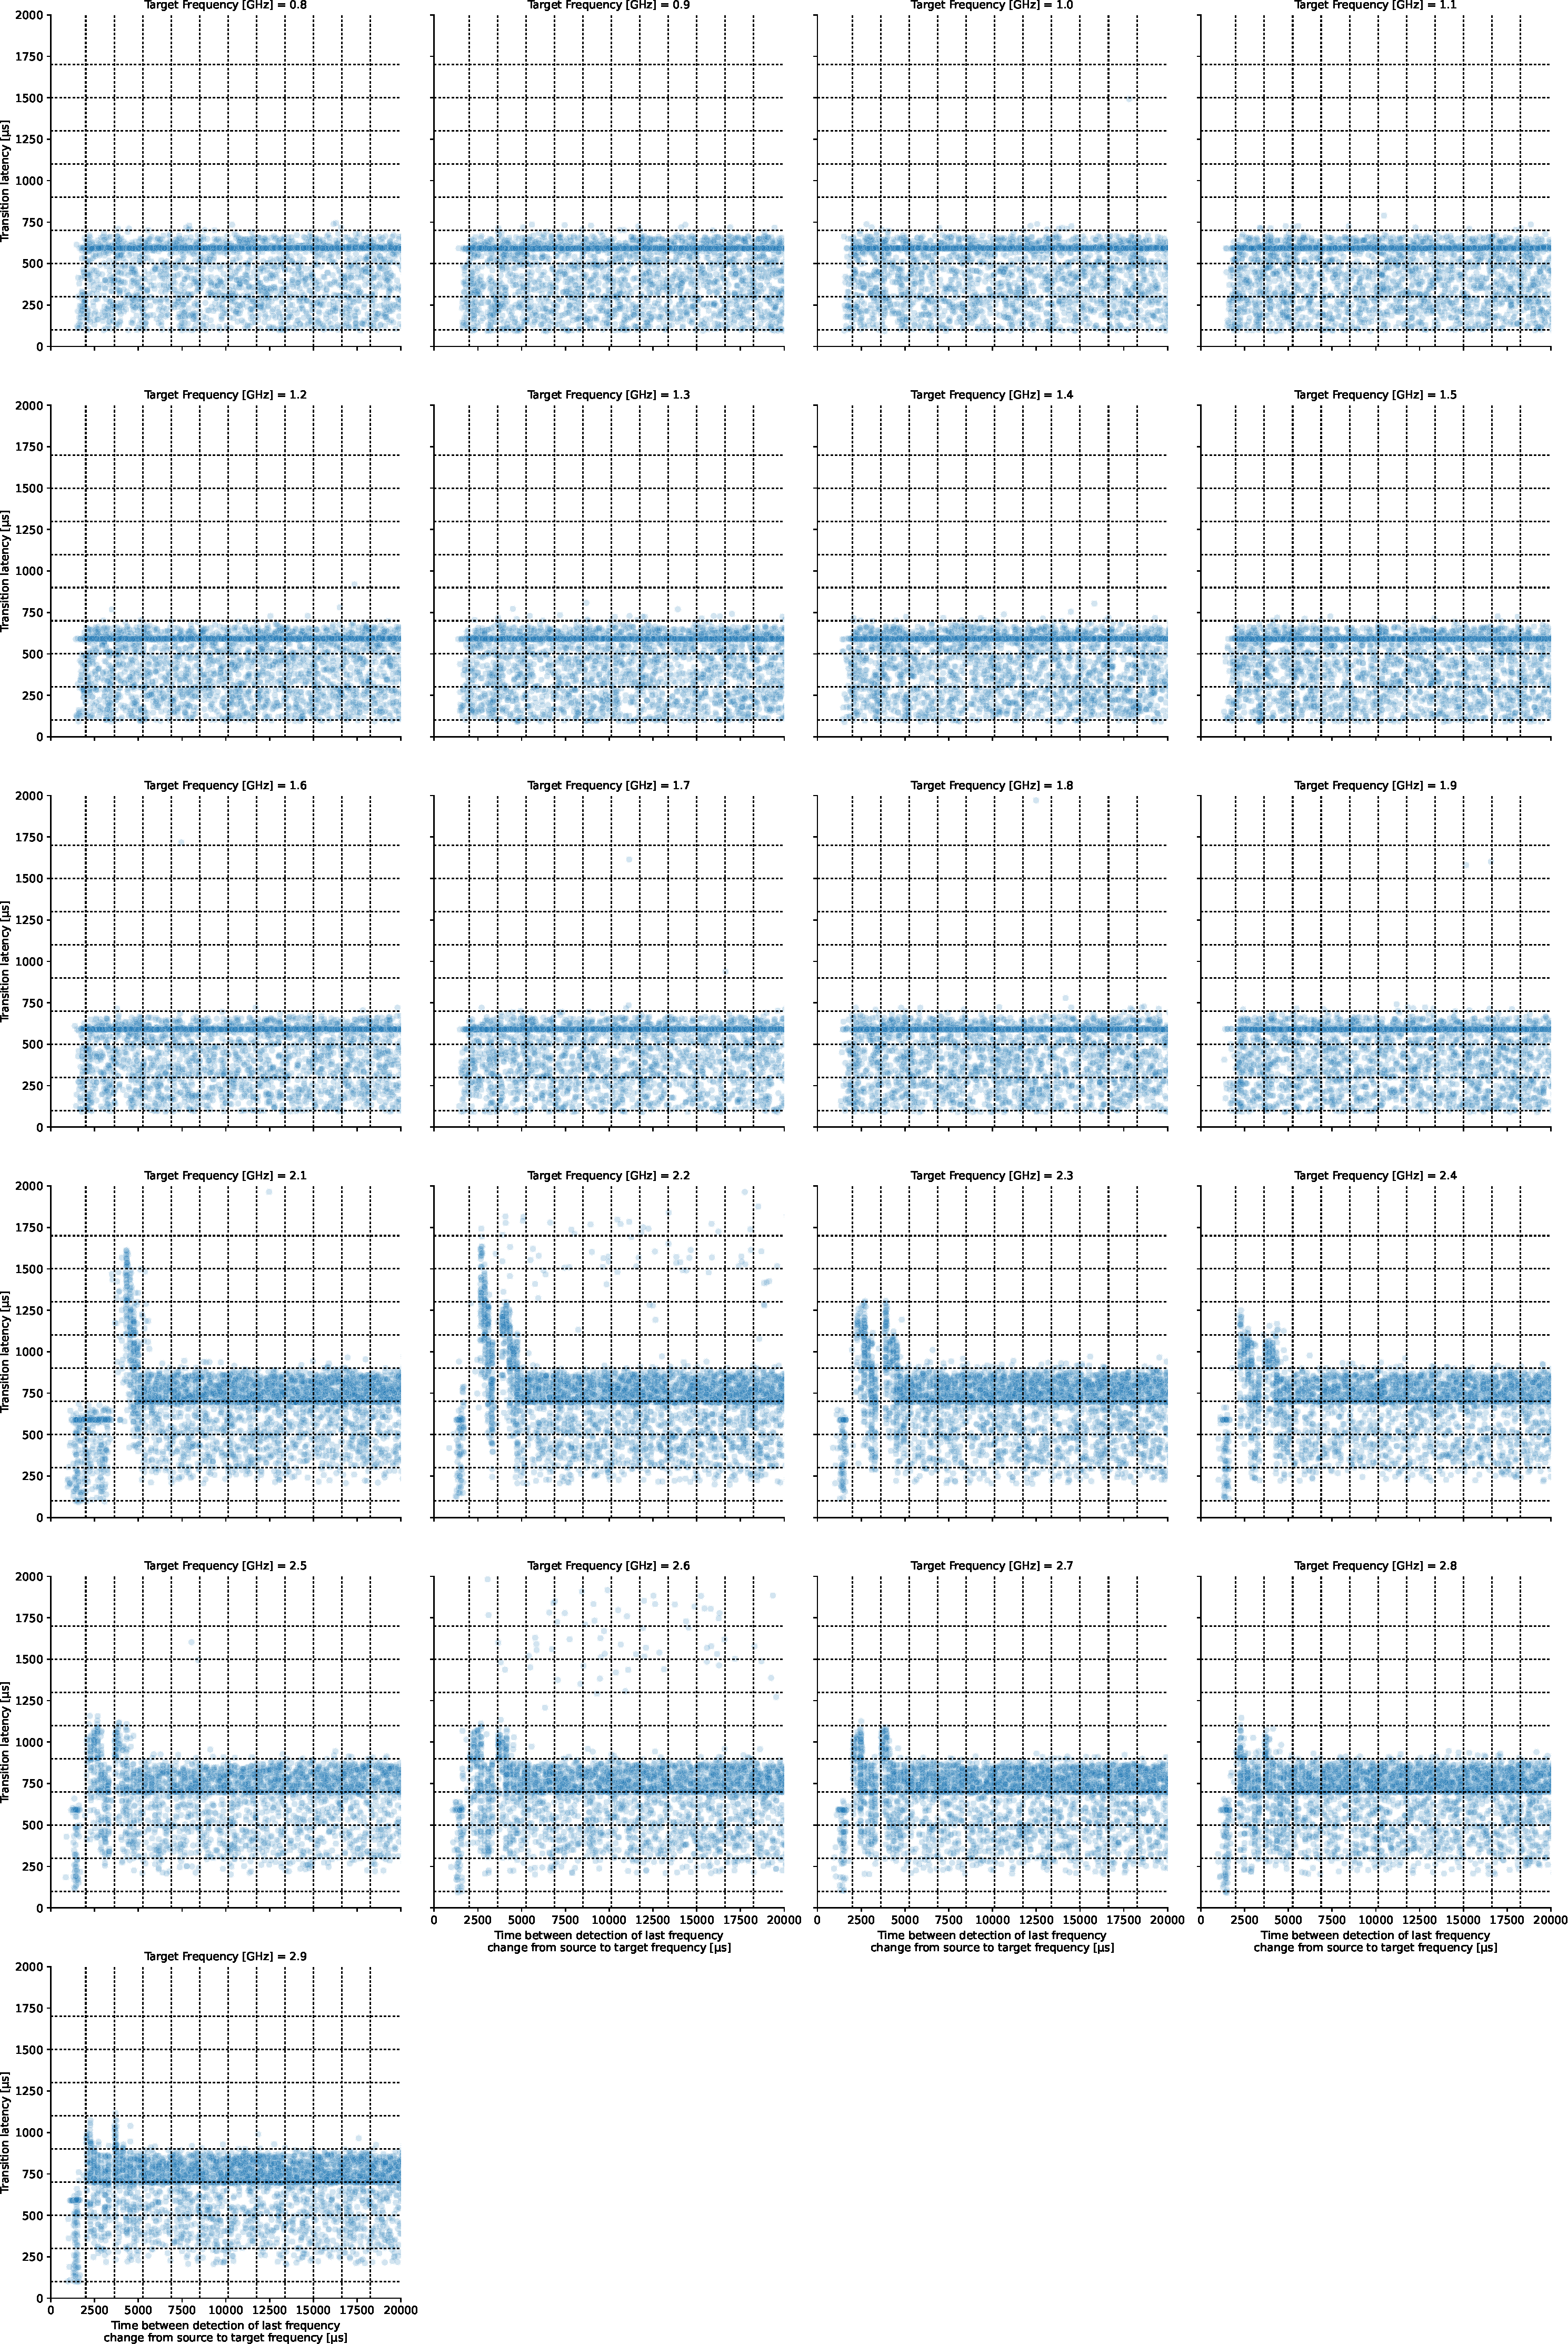
\includegraphics[width=\columnwidth]{fig/ftalat_scatter_wait_transition_latency_hati_source_2.0.pdf}
    \caption{Dependance of the time between the detection events of transitions from \SI{2.0}{\GHz} to \SI{0.8}{}, \SI{0.9}{}, ..., \SI{2.9}{\GHz}. For better lines for bins of size \SI{1625}{\us} and \SI{200}{\us} have been included for the x and y-axis respectively.}
\end{figure}
\begin{figure}[]
    \centering
    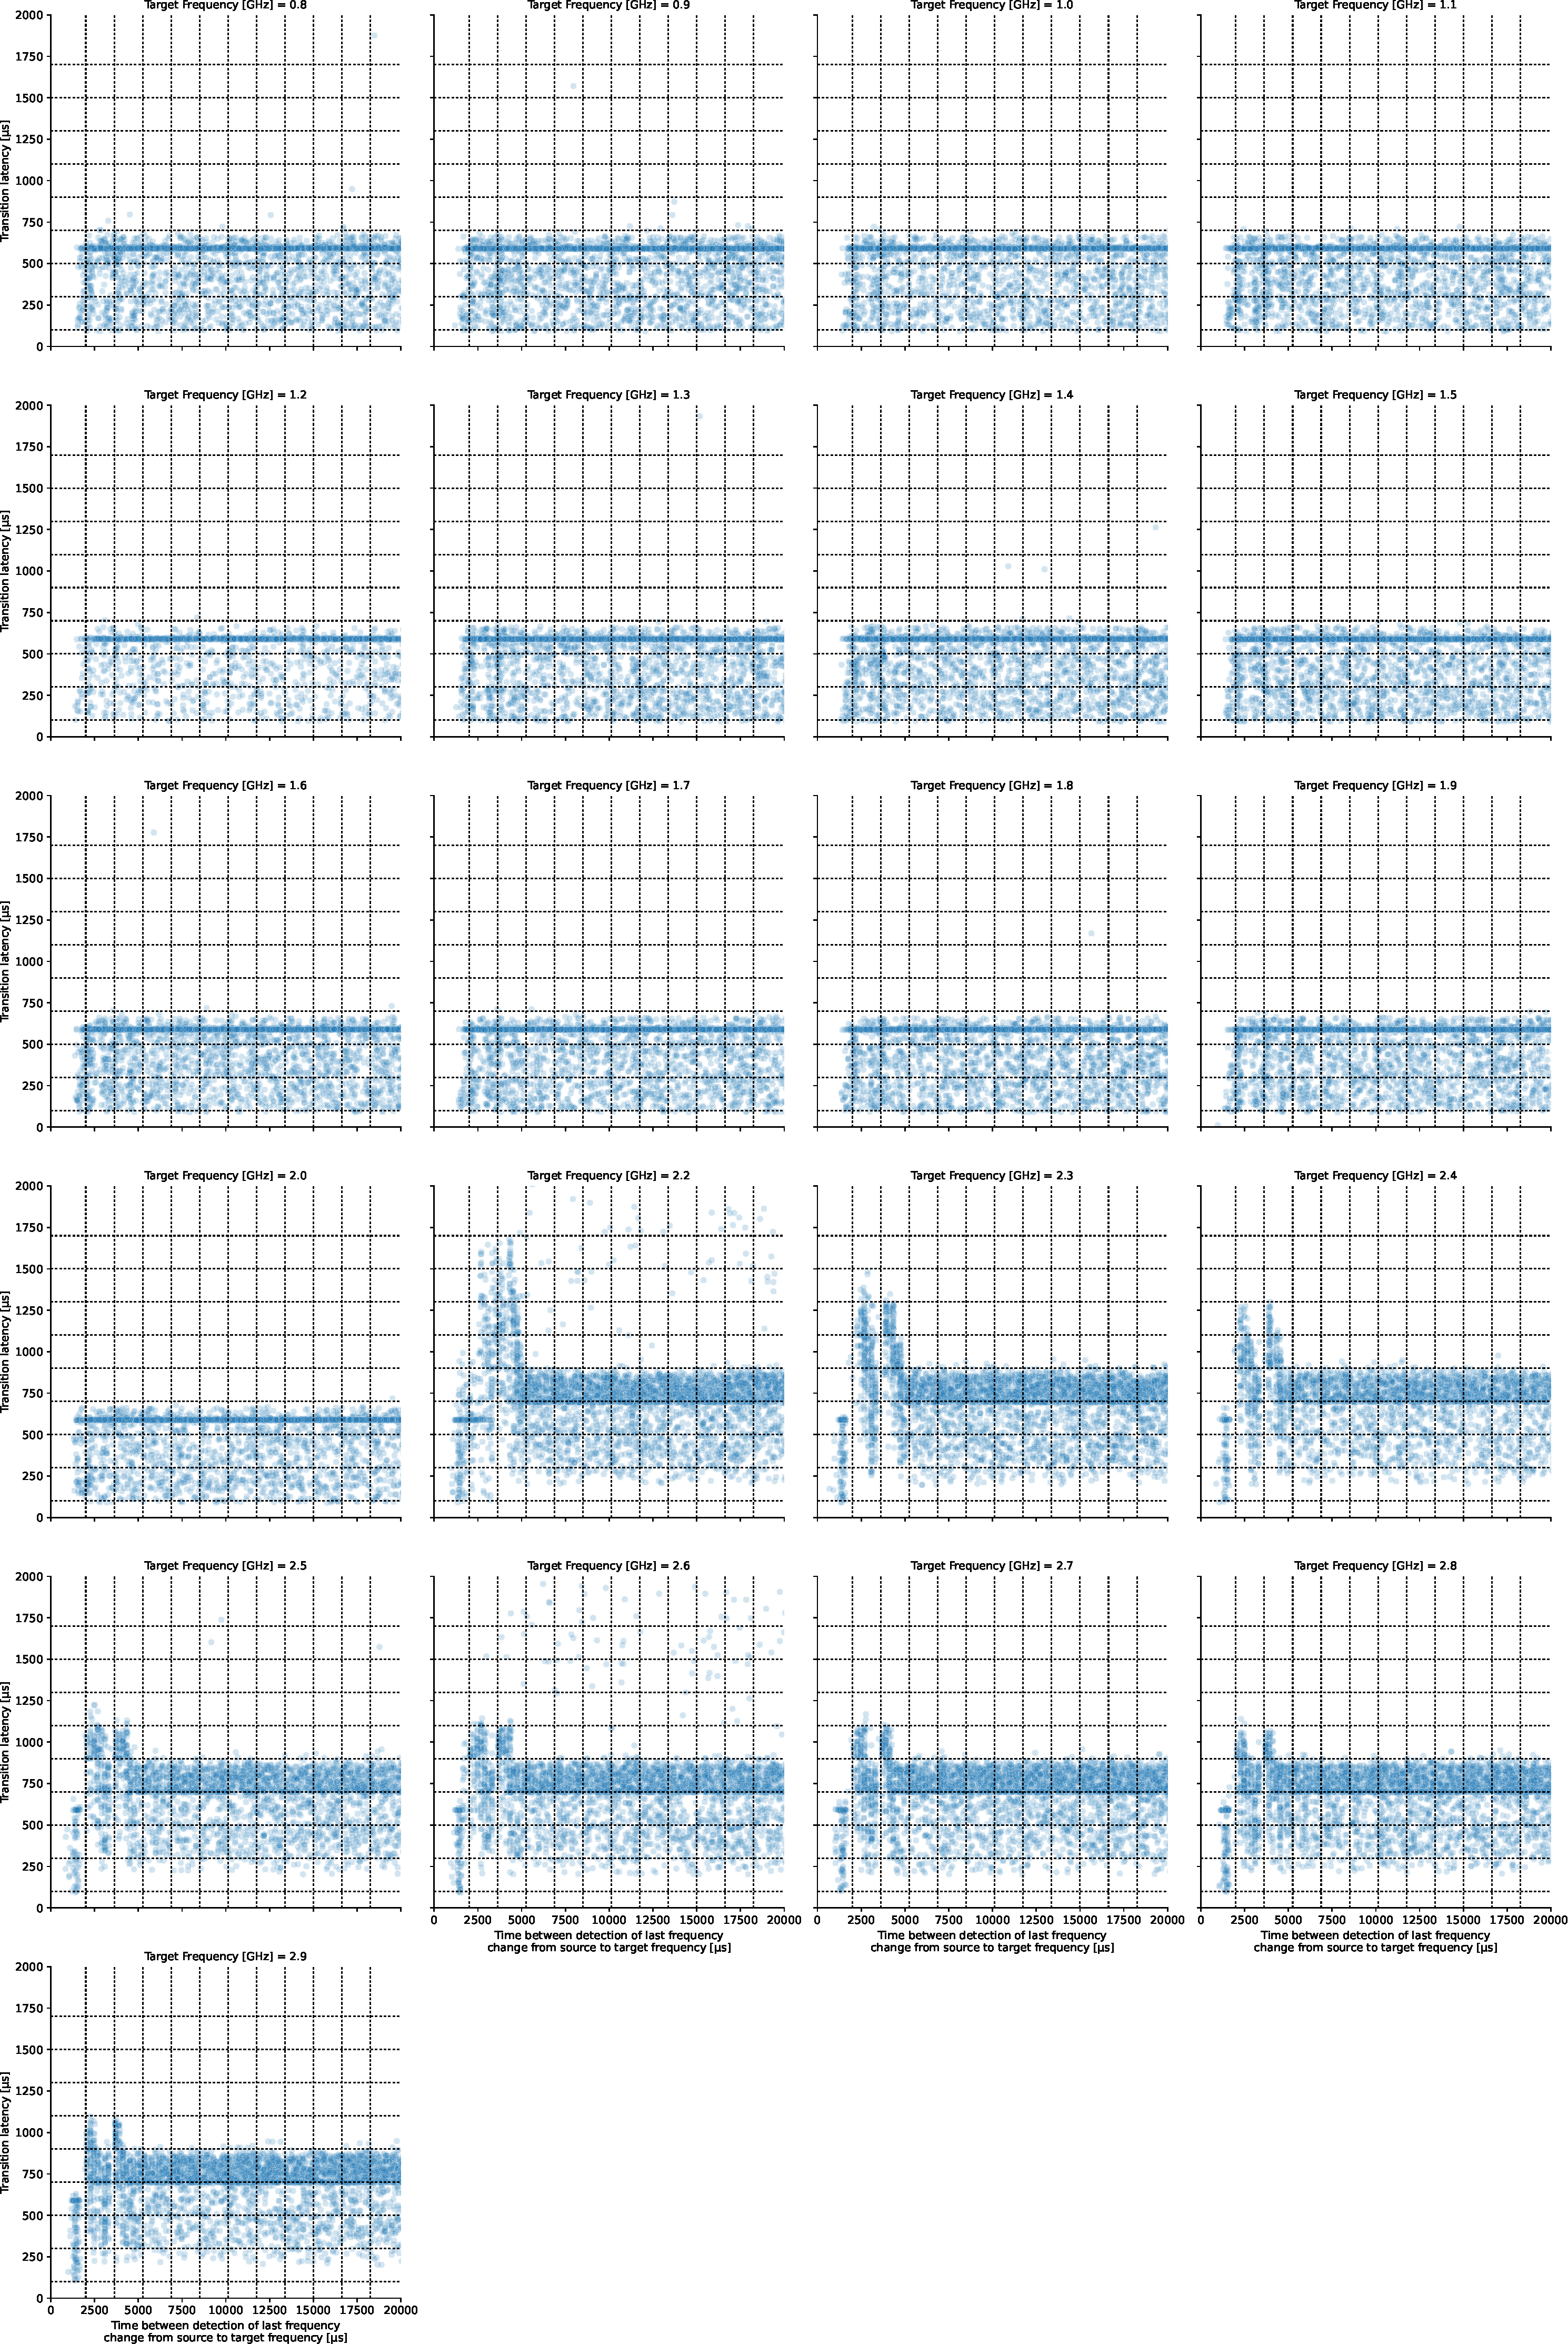
\includegraphics[width=\columnwidth]{fig/ftalat_scatter_wait_transition_latency_hati_source_2.1.pdf}
    \caption{Dependance of the time between the detection events of transitions from \SI{2.1}{\GHz} to \SI{0.8}{}, \SI{0.9}{}, ..., \SI{2.9}{\GHz}. For better lines for bins of size \SI{1625}{\us} and \SI{200}{\us} have been included for the x and y-axis respectively.}
\end{figure}
\begin{figure}[]
    \centering
    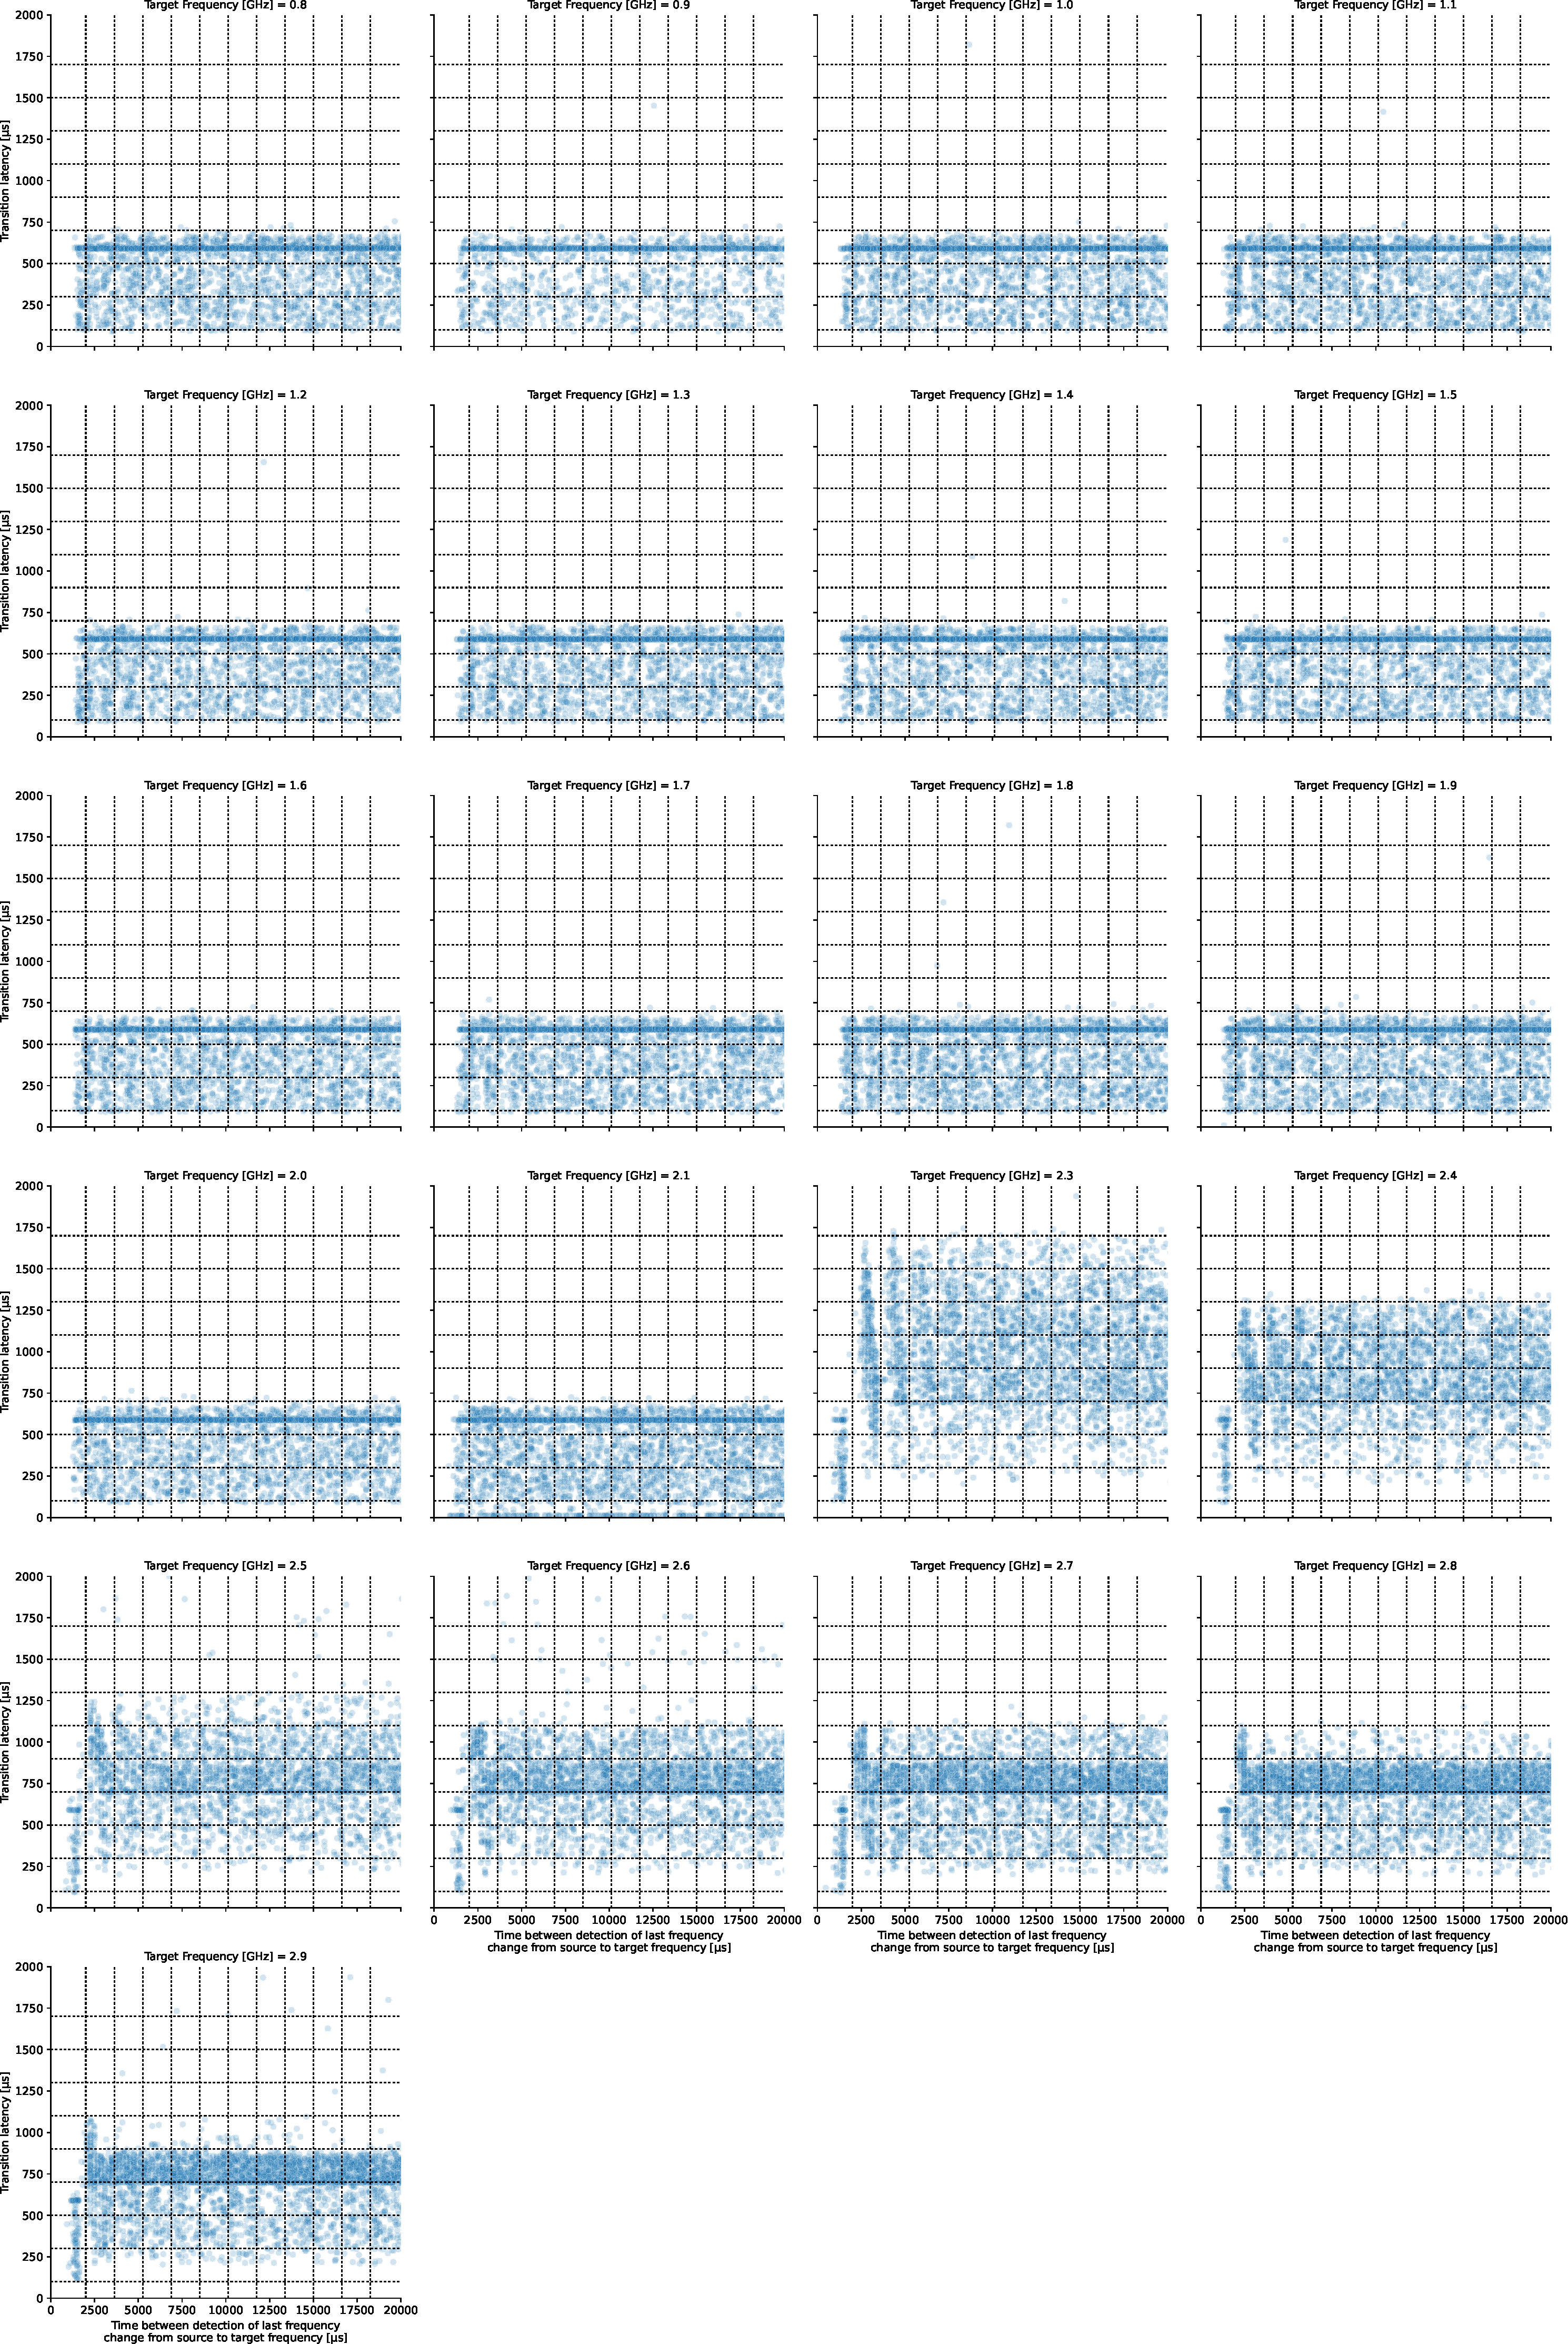
\includegraphics[width=\columnwidth]{fig/ftalat_scatter_wait_transition_latency_hati_source_2.2.pdf}
    \caption{Dependance of the time between the detection events of transitions from \SI{2.2}{\GHz} to \SI{0.8}{}, \SI{0.9}{}, ..., \SI{2.9}{\GHz}. For better lines for bins of size \SI{1625}{\us} and \SI{200}{\us} have been included for the x and y-axis respectively.}
\end{figure}
\begin{figure}[]
    \centering
    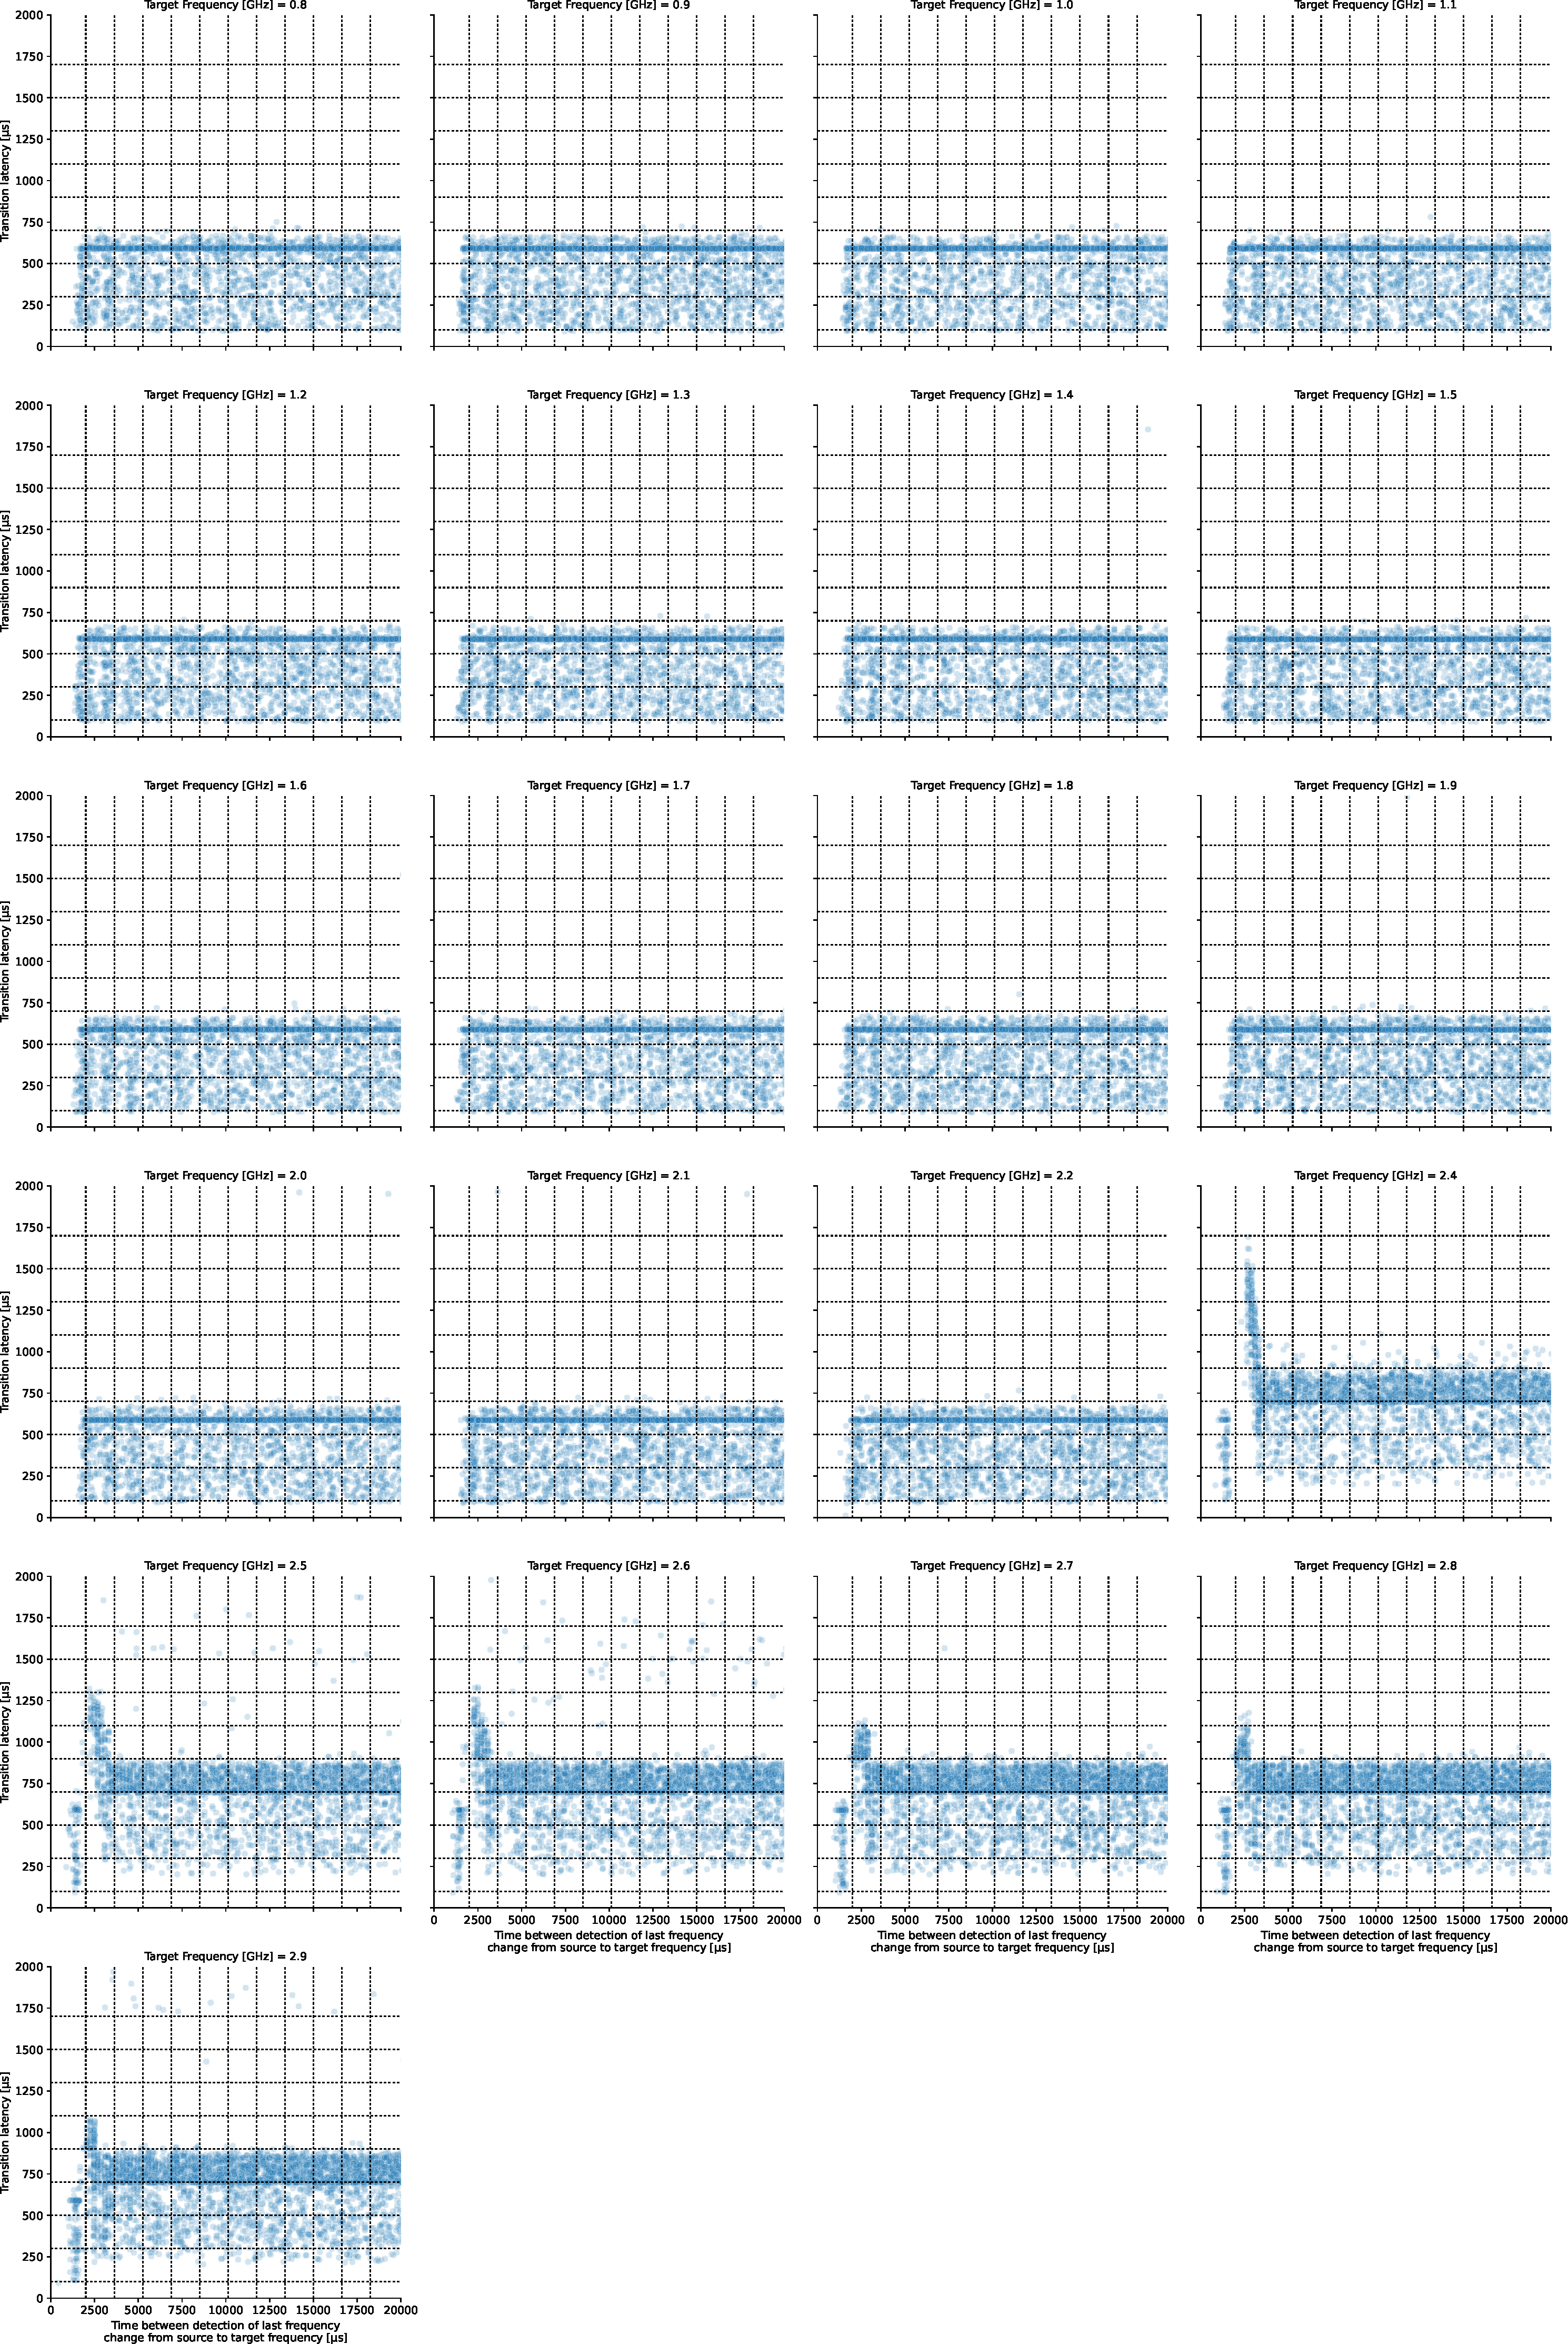
\includegraphics[width=\columnwidth]{fig/ftalat_scatter_wait_transition_latency_hati_source_2.3.pdf}
    \caption{Dependance of the time between the detection events of transitions from \SI{2.3}{\GHz} to \SI{0.8}{}, \SI{0.9}{}, ..., \SI{2.9}{\GHz}. For better lines for bins of size \SI{1625}{\us} and \SI{200}{\us} have been included for the x and y-axis respectively.}
\end{figure}
\begin{figure}[]
    \centering
    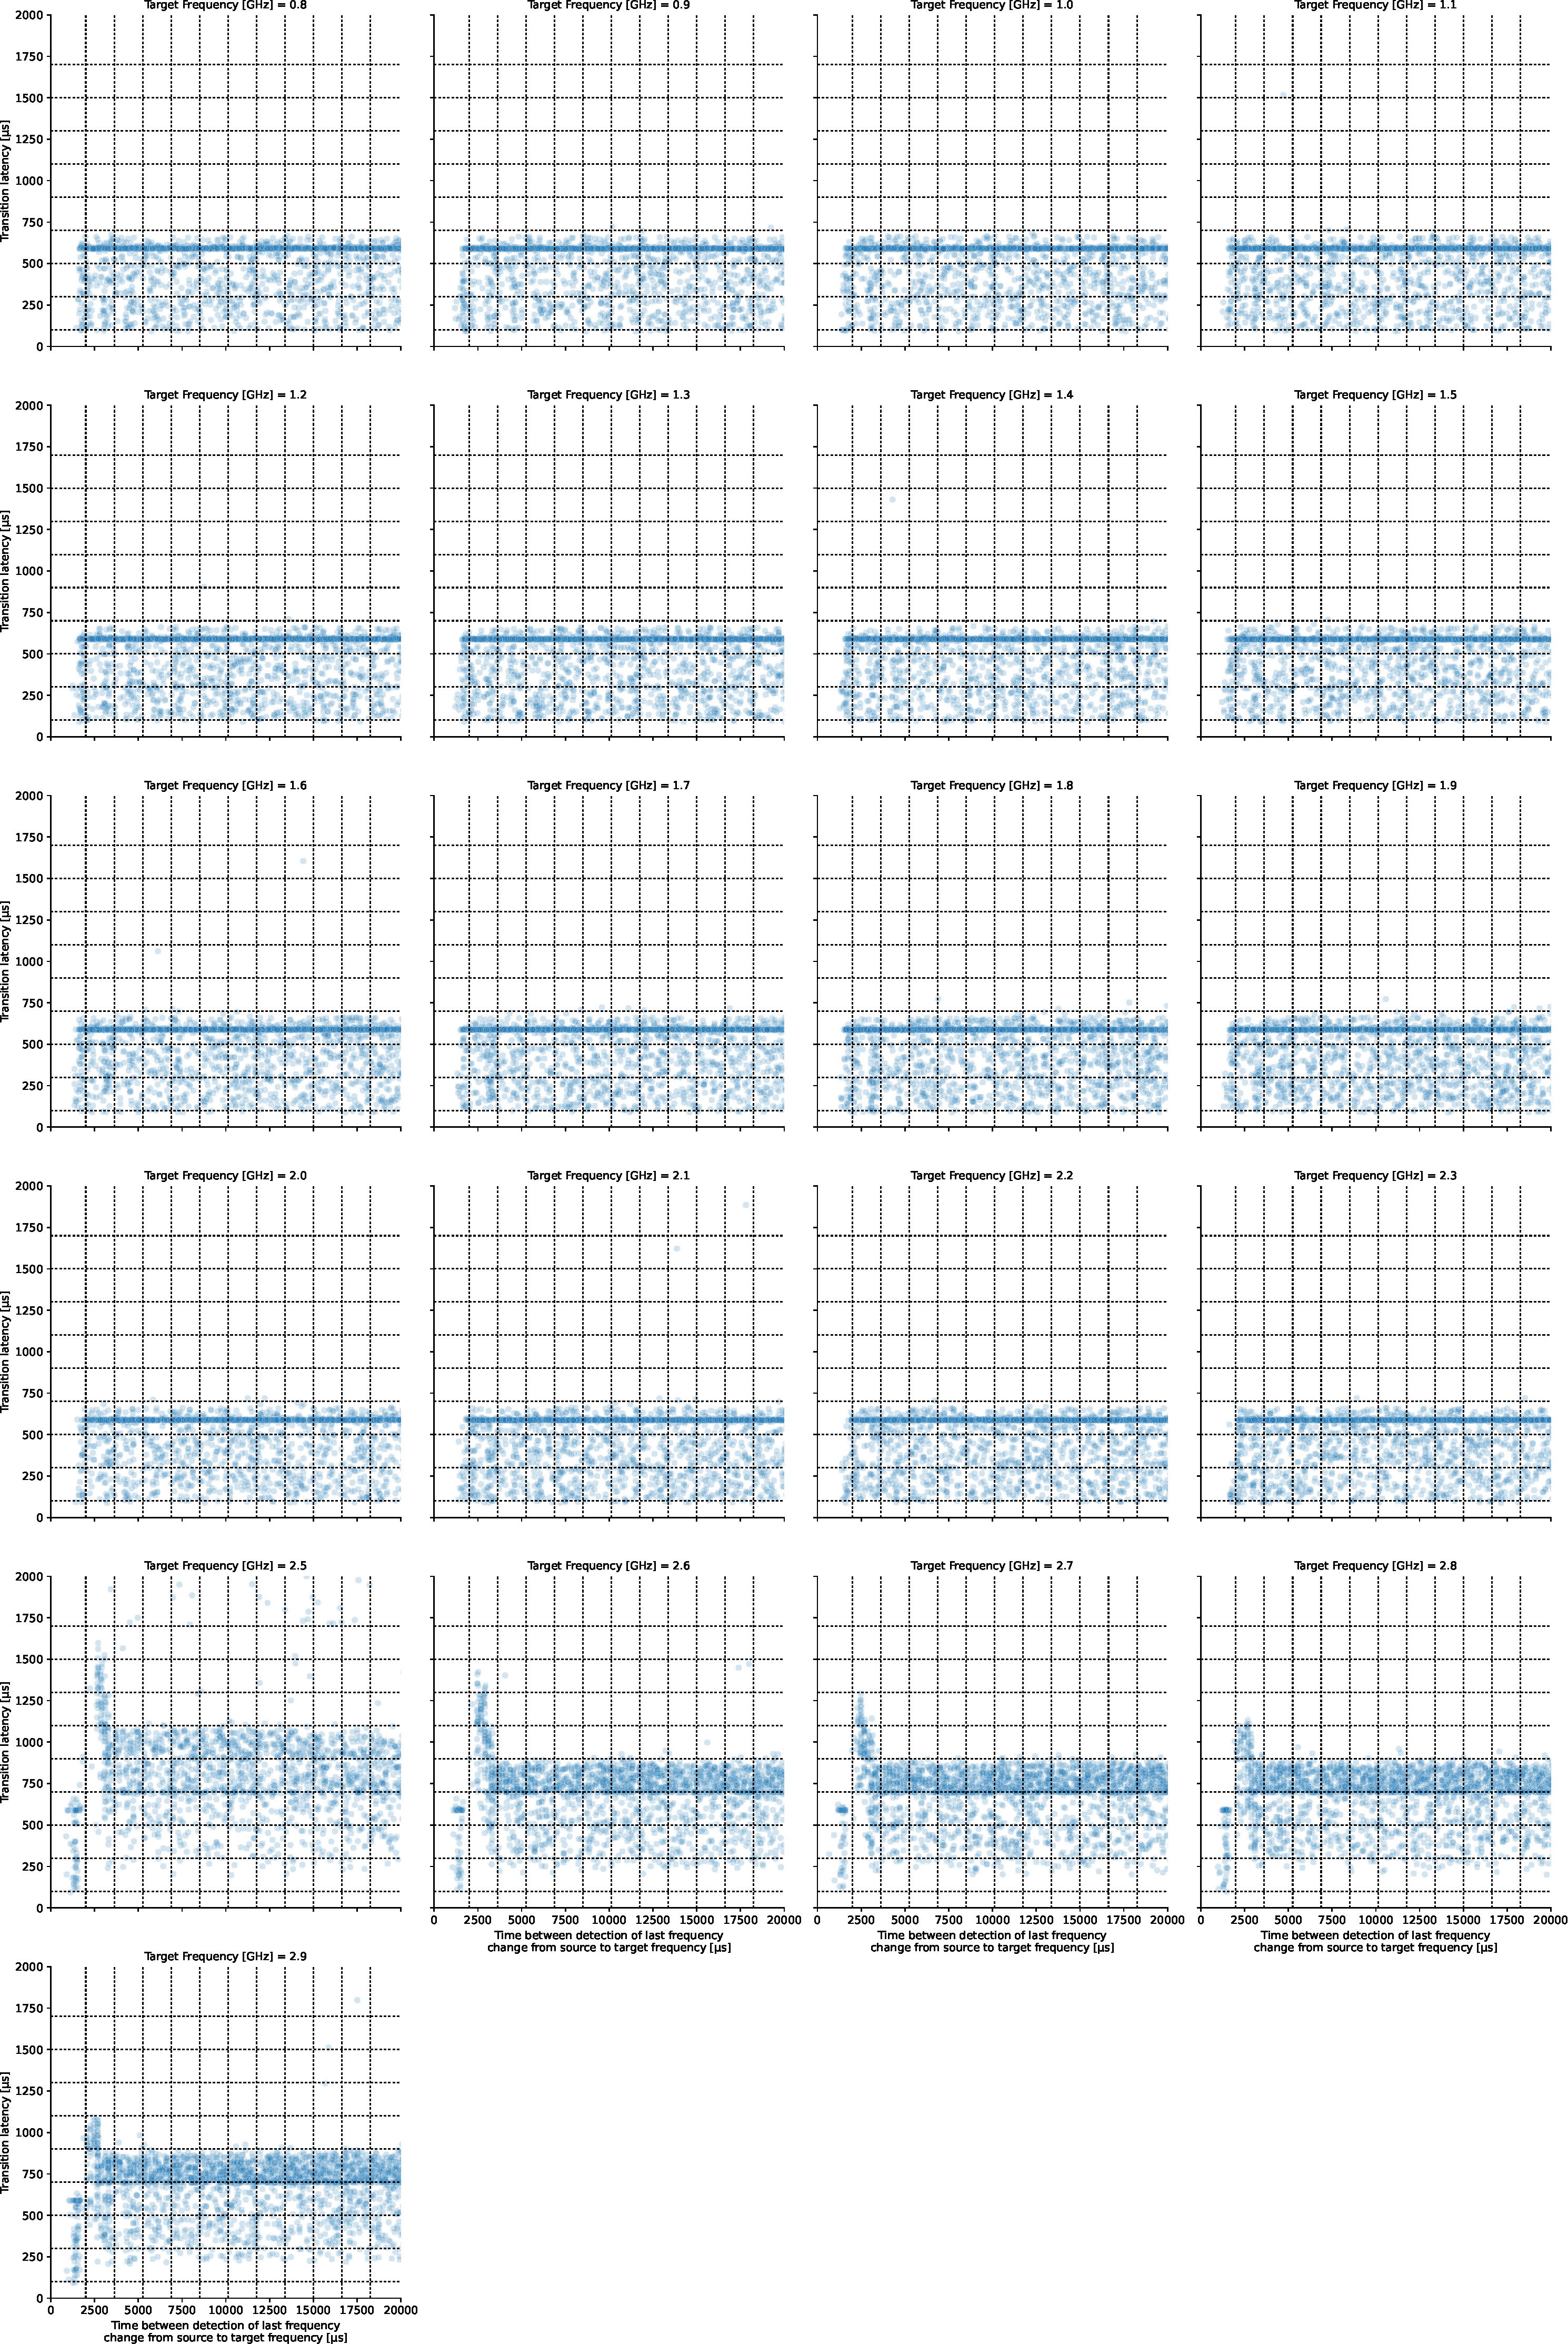
\includegraphics[width=\columnwidth]{fig/ftalat_scatter_wait_transition_latency_hati_source_2.4.pdf}
    \caption{Dependance of the time between the detection events of transitions from \SI{2.4}{\GHz} to \SI{0.8}{}, \SI{0.9}{}, ..., \SI{2.9}{\GHz}. For better lines for bins of size \SI{1625}{\us} and \SI{200}{\us} have been included for the x and y-axis respectively.}
\end{figure}
\begin{figure}[]
    \centering
    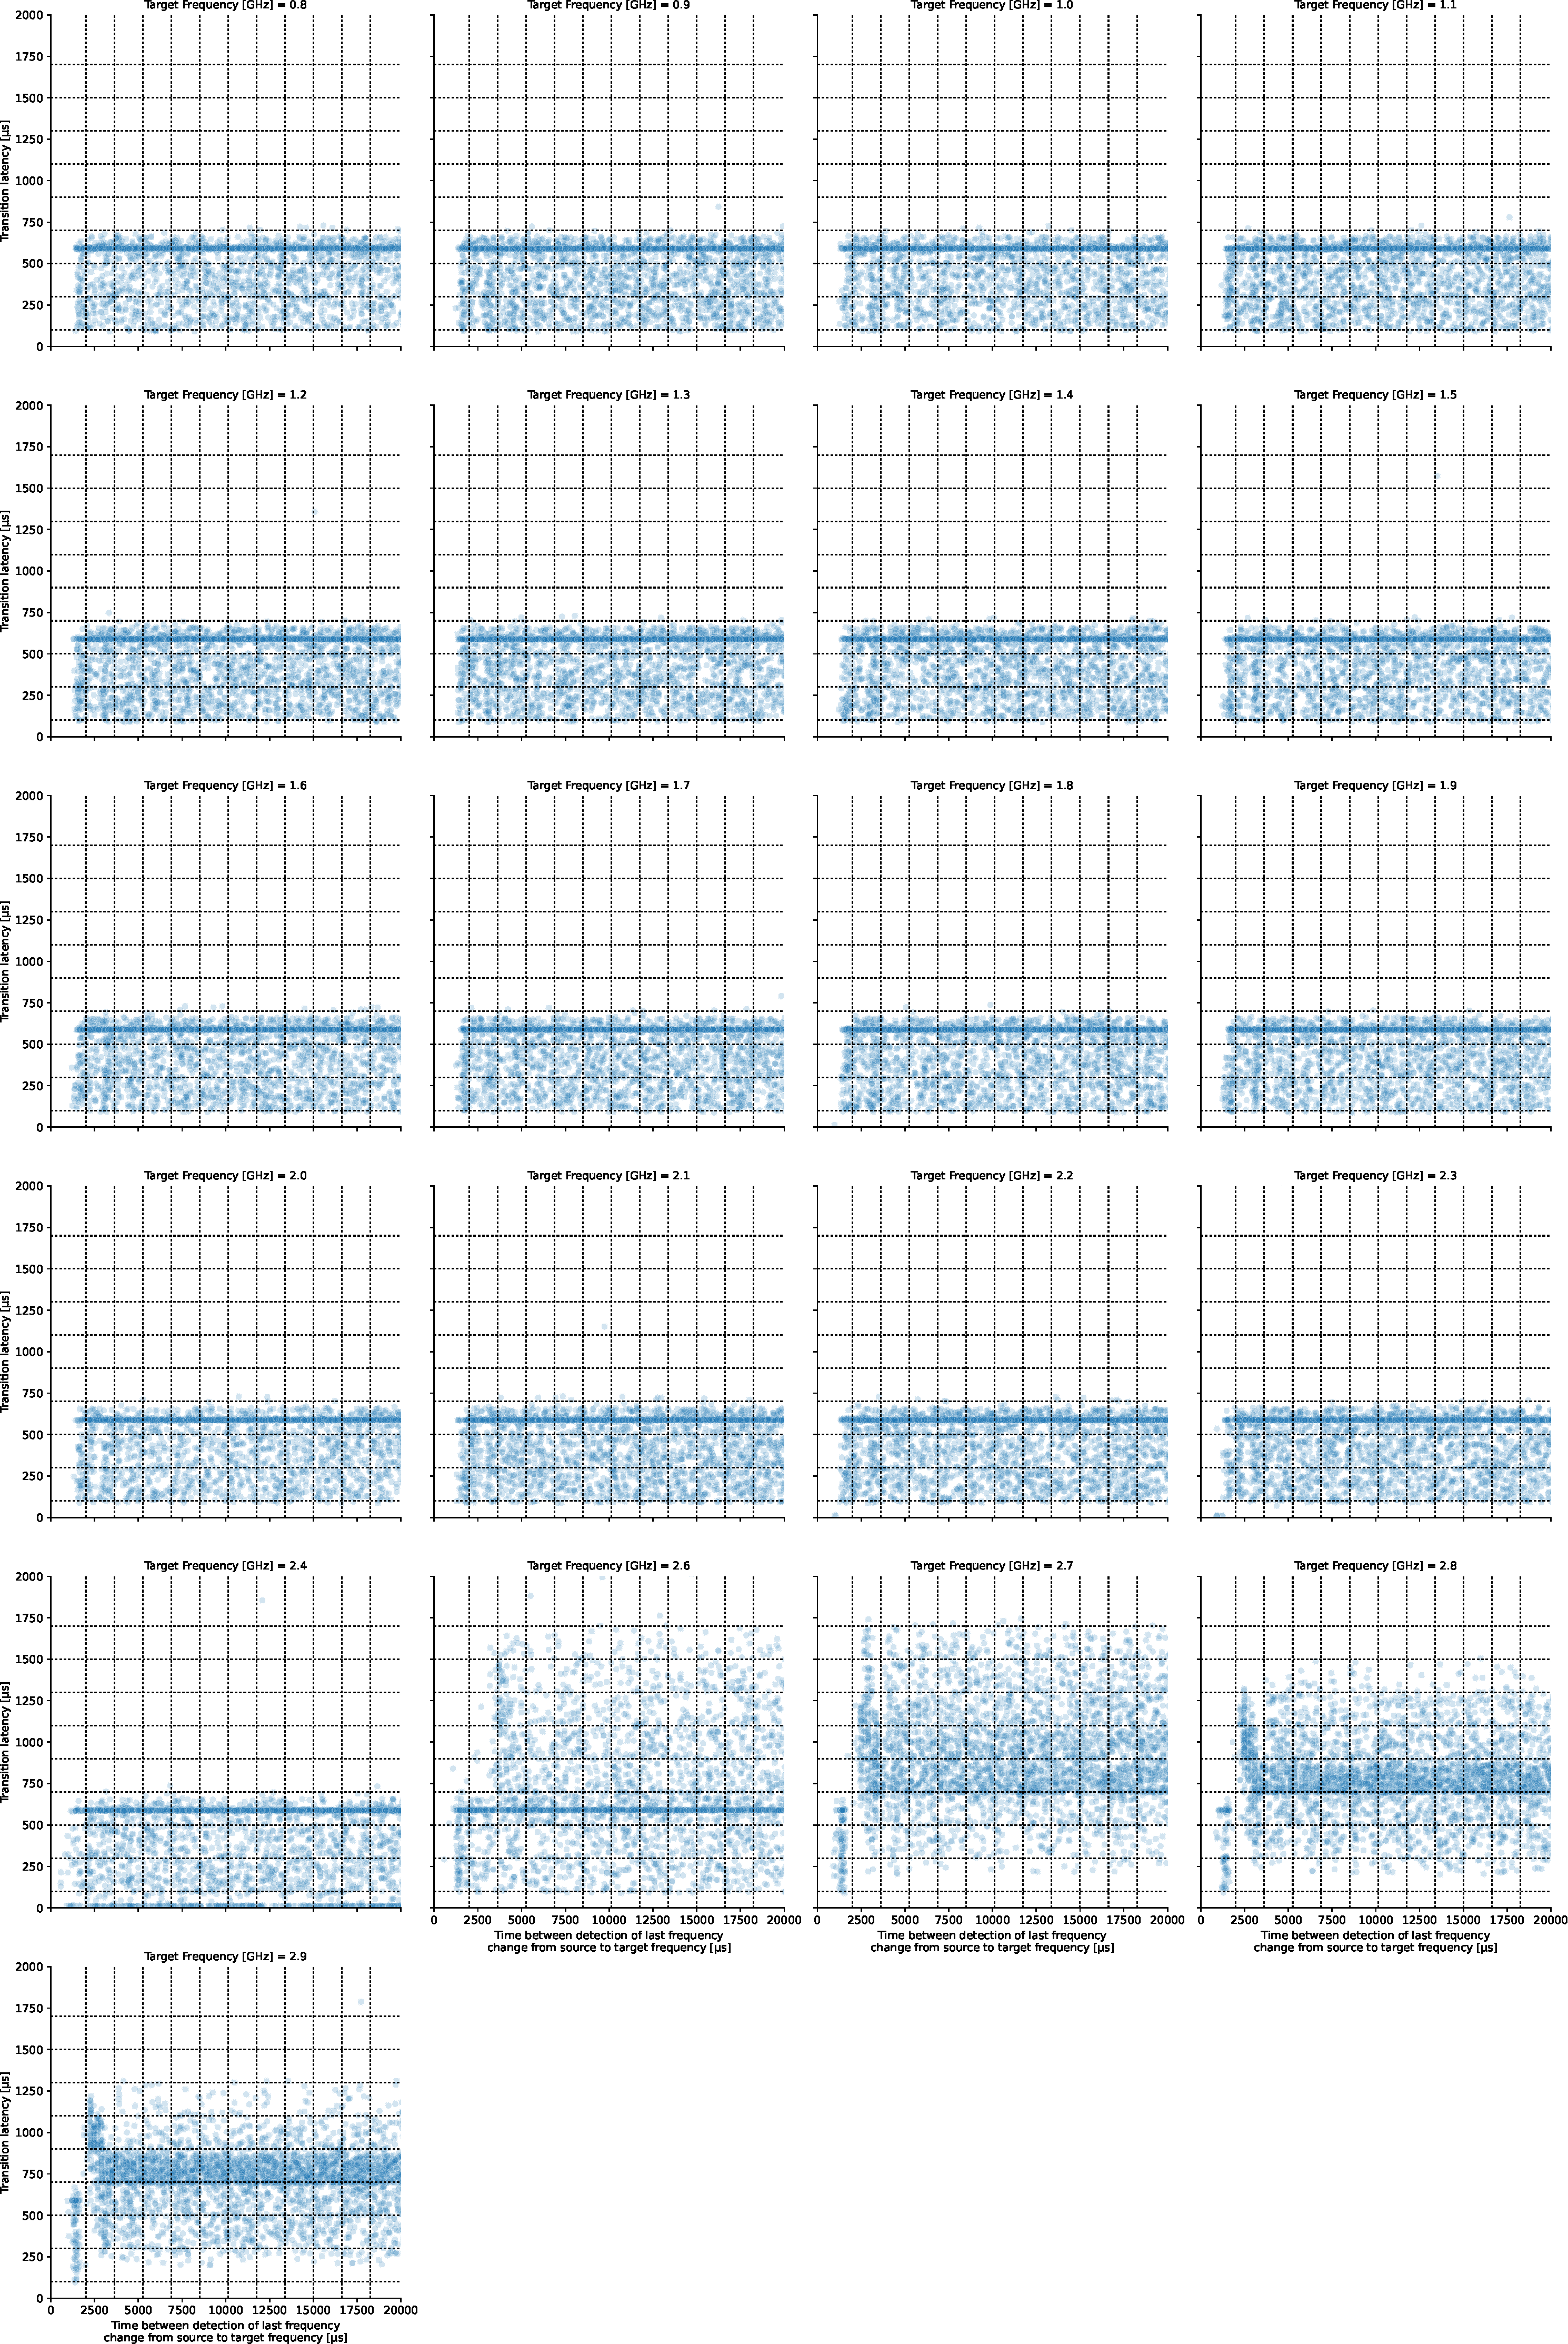
\includegraphics[width=\columnwidth]{fig/ftalat_scatter_wait_transition_latency_hati_source_2.5.pdf}
    \caption{Dependance of the time between the detection events of transitions from \SI{2.5}{\GHz} to \SI{0.8}{}, \SI{0.9}{}, ..., \SI{2.9}{\GHz}. For better lines for bins of size \SI{1625}{\us} and \SI{200}{\us} have been included for the x and y-axis respectively.}
\end{figure}
\begin{figure}[]
    \centering
    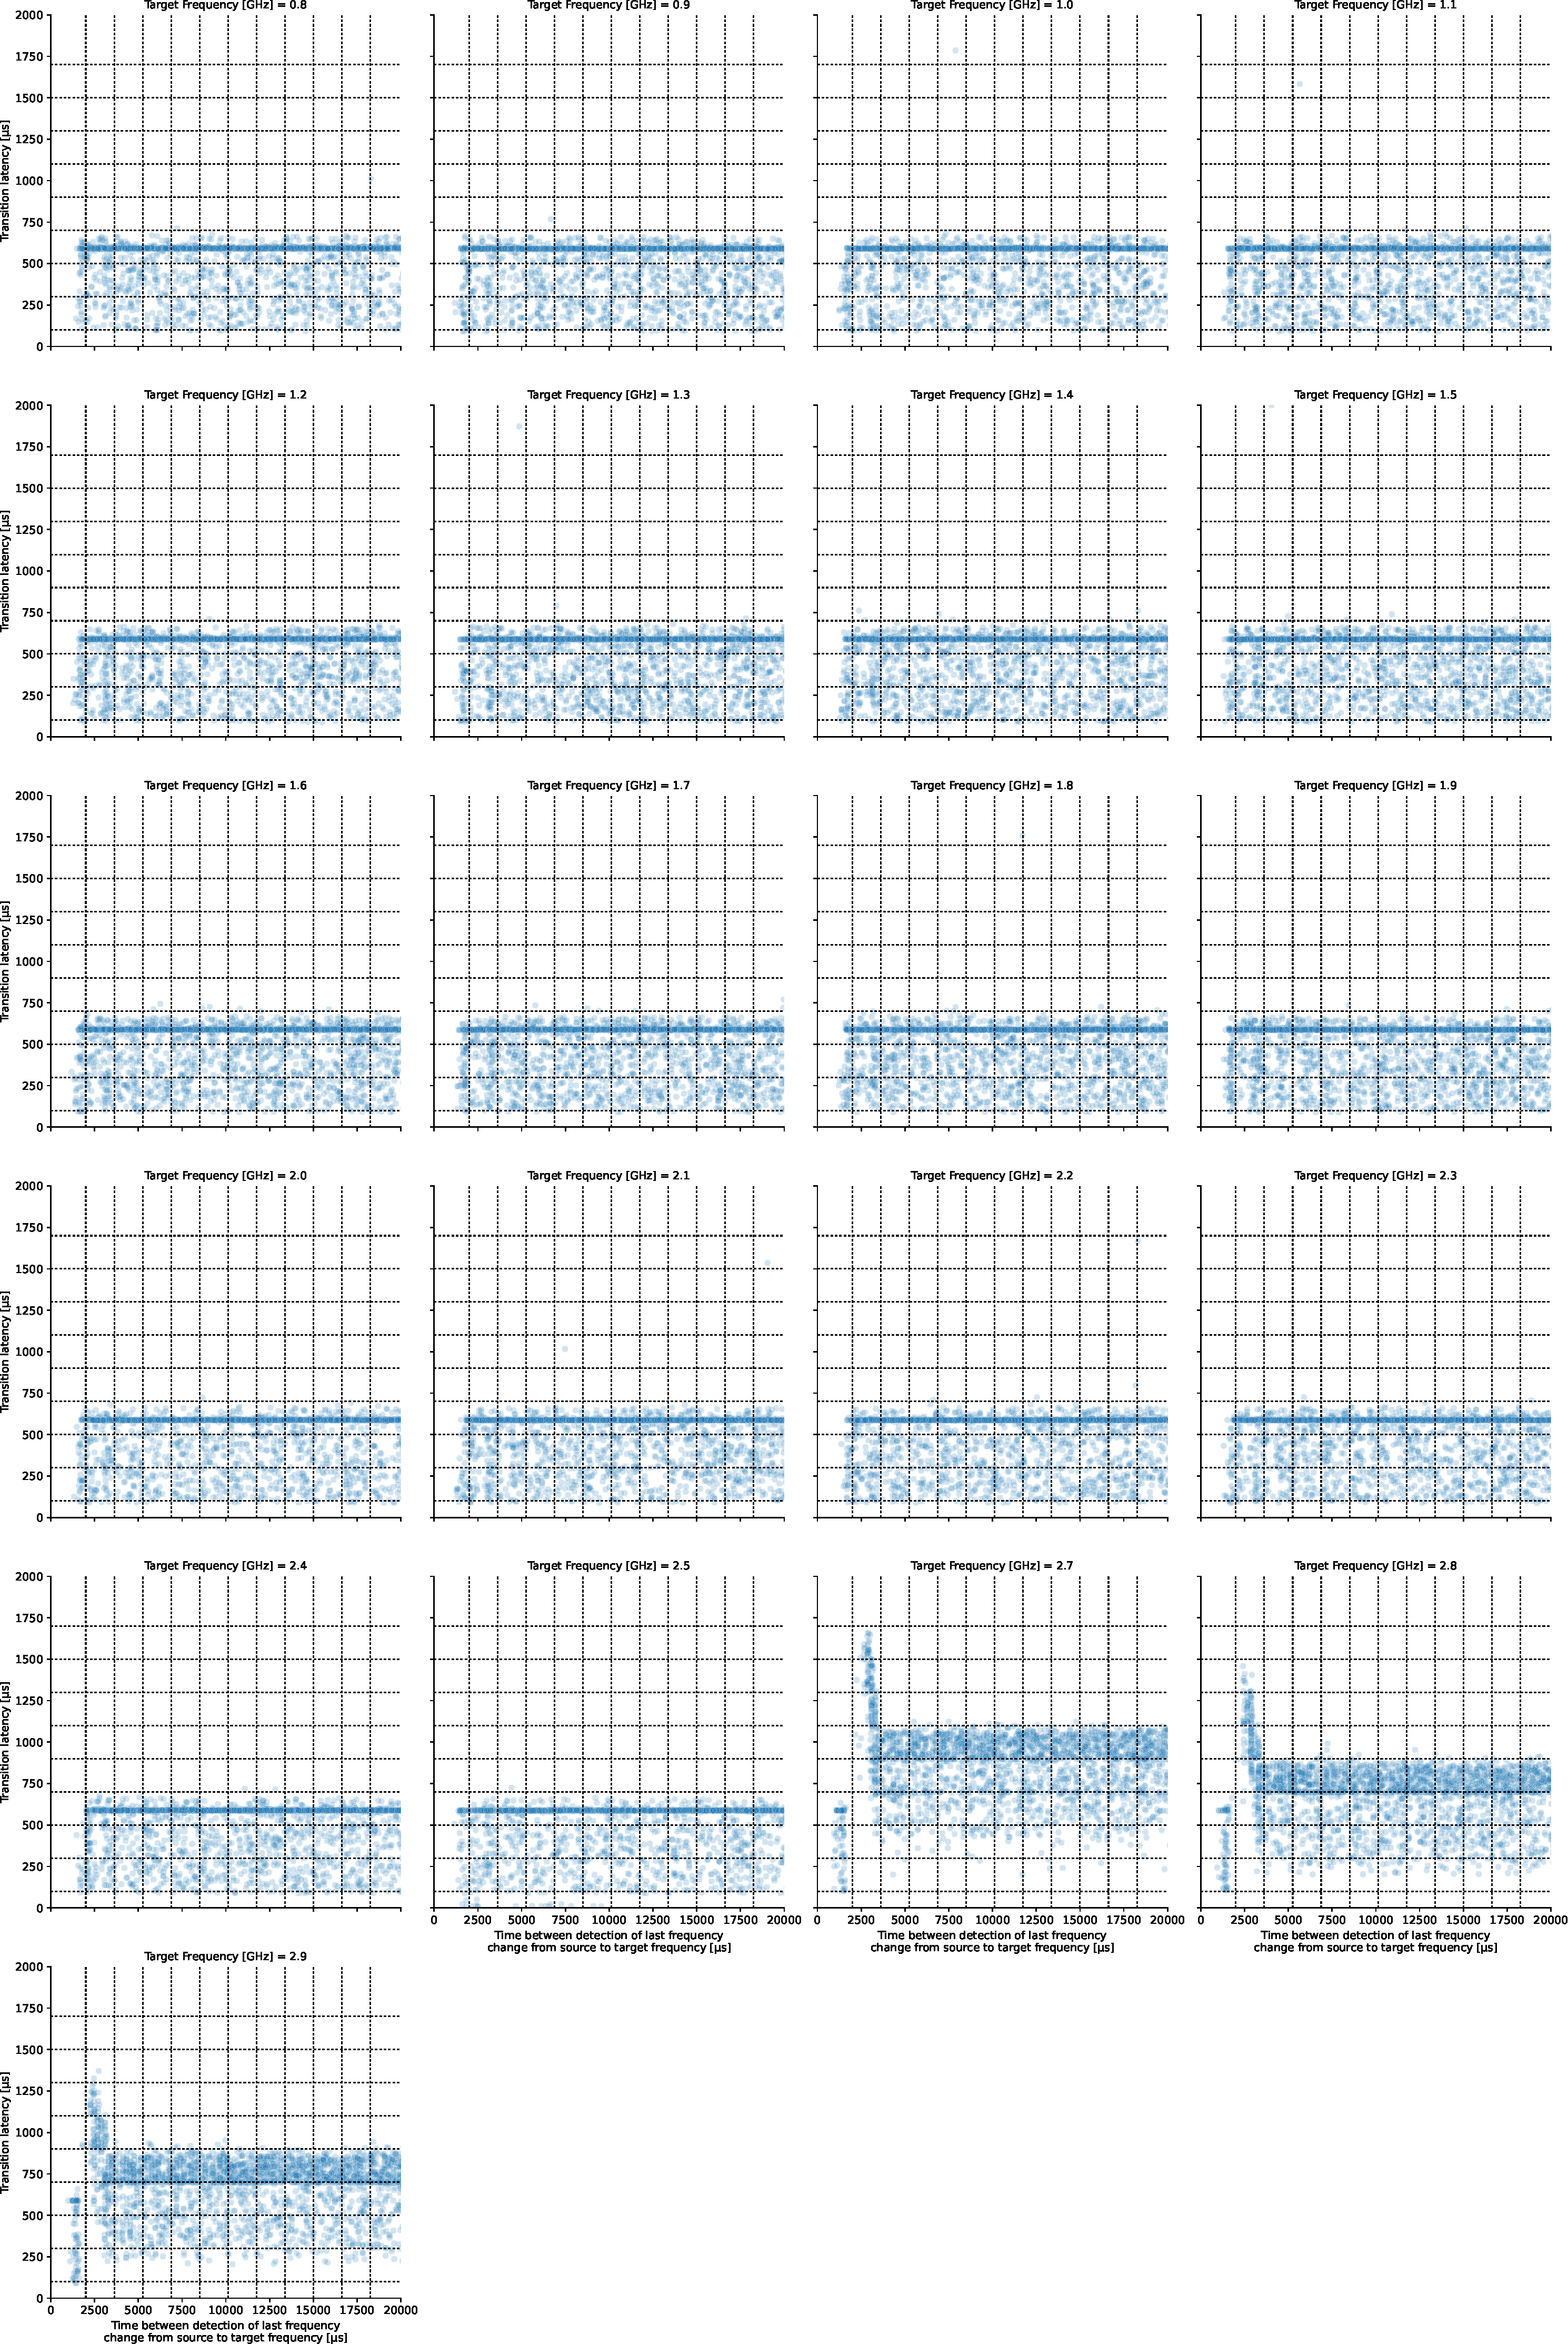
\includegraphics[width=\columnwidth]{fig/ftalat_scatter_wait_transition_latency_hati_source_2.6.pdf}
    \caption{Dependance of the time between the detection events of transitions from \SI{2.6}{\GHz} to \SI{0.8}{}, \SI{0.9}{}, ..., \SI{2.9}{\GHz}. For better lines for bins of size \SI{1625}{\us} and \SI{200}{\us} have been included for the x and y-axis respectively.}
\end{figure}
\begin{figure}[]
    \centering
    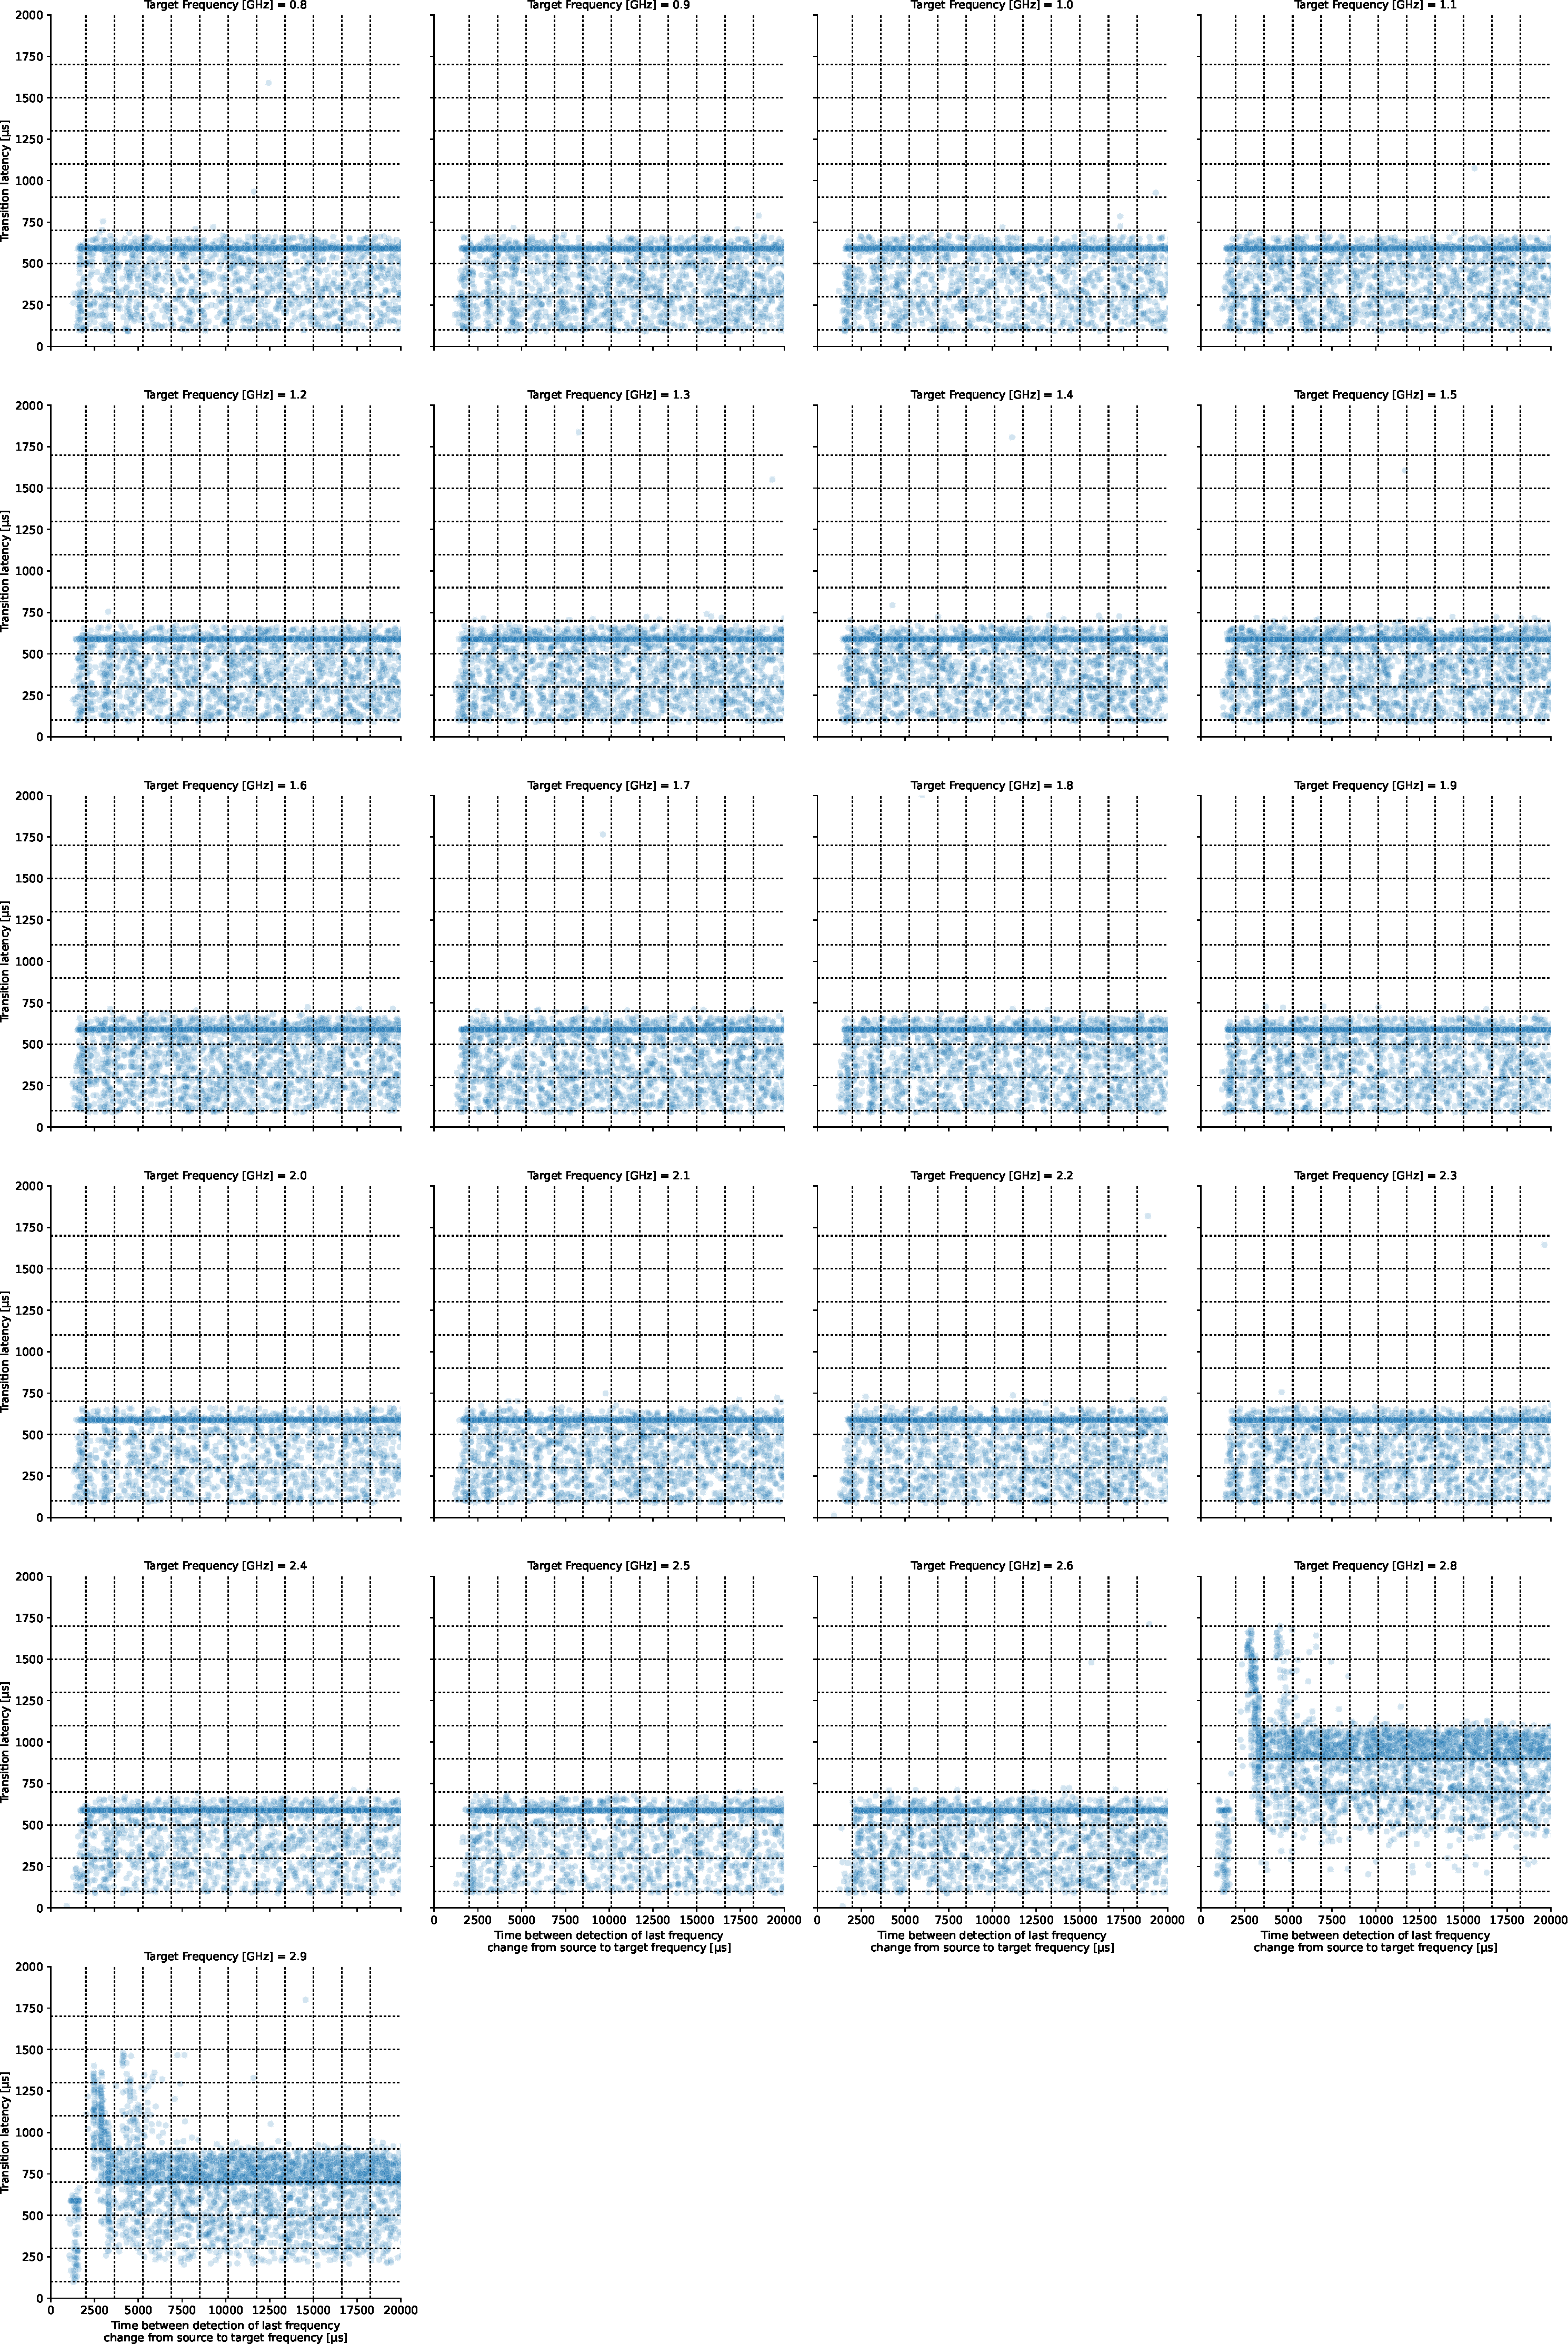
\includegraphics[width=\columnwidth]{fig/ftalat_scatter_wait_transition_latency_hati_source_2.7.pdf}
    \caption{Dependance of the time between the detection events of transitions from \SI{2.7}{\GHz} to \SI{0.8}{}, \SI{0.9}{}, ..., \SI{2.9}{\GHz}. For better lines for bins of size \SI{1625}{\us} and \SI{200}{\us} have been included for the x and y-axis respectively.}
\end{figure}
\begin{figure}[]
    \centering
    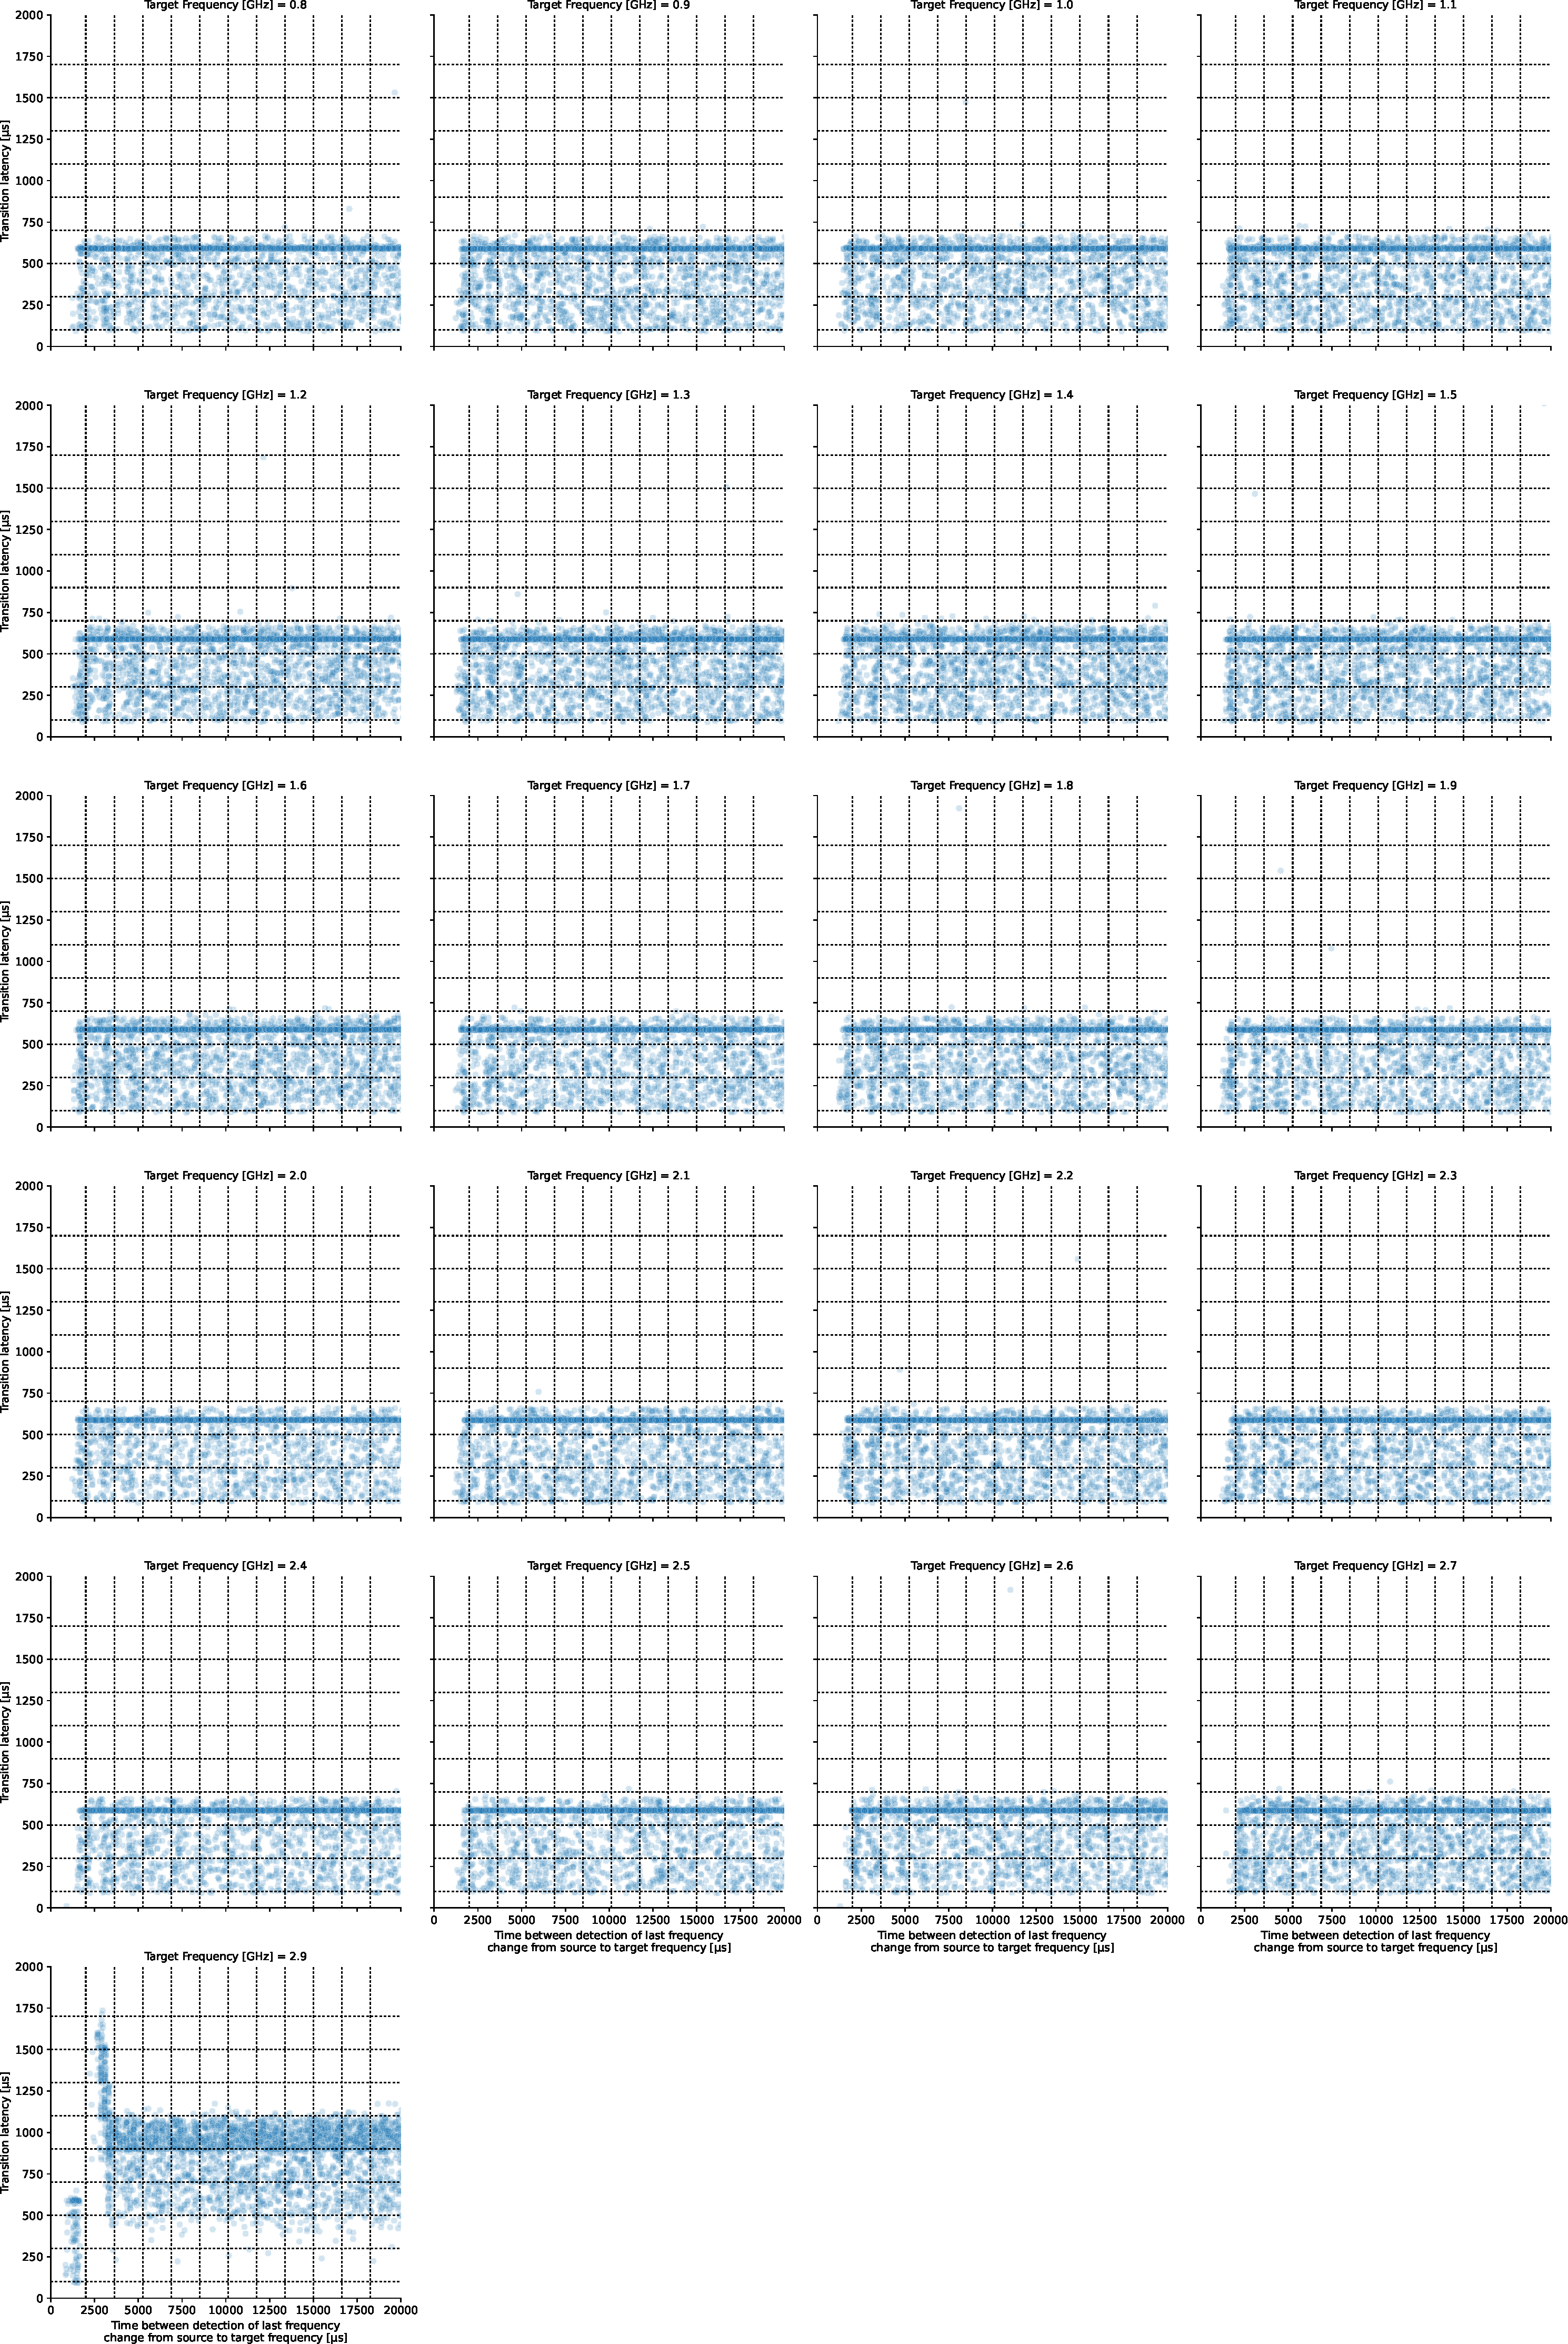
\includegraphics[width=\columnwidth]{fig/ftalat_scatter_wait_transition_latency_hati_source_2.8.pdf}
    \caption{Dependance of the time between the detection events of transitions from \SI{2.8}{\GHz} to \SI{0.8}{}, \SI{0.9}{}, ..., \SI{2.9}{\GHz}. For better lines for bins of size \SI{1625}{\us} and \SI{200}{\us} have been included for the x and y-axis respectively.}
\end{figure}
\begin{figure}[]
    \centering
    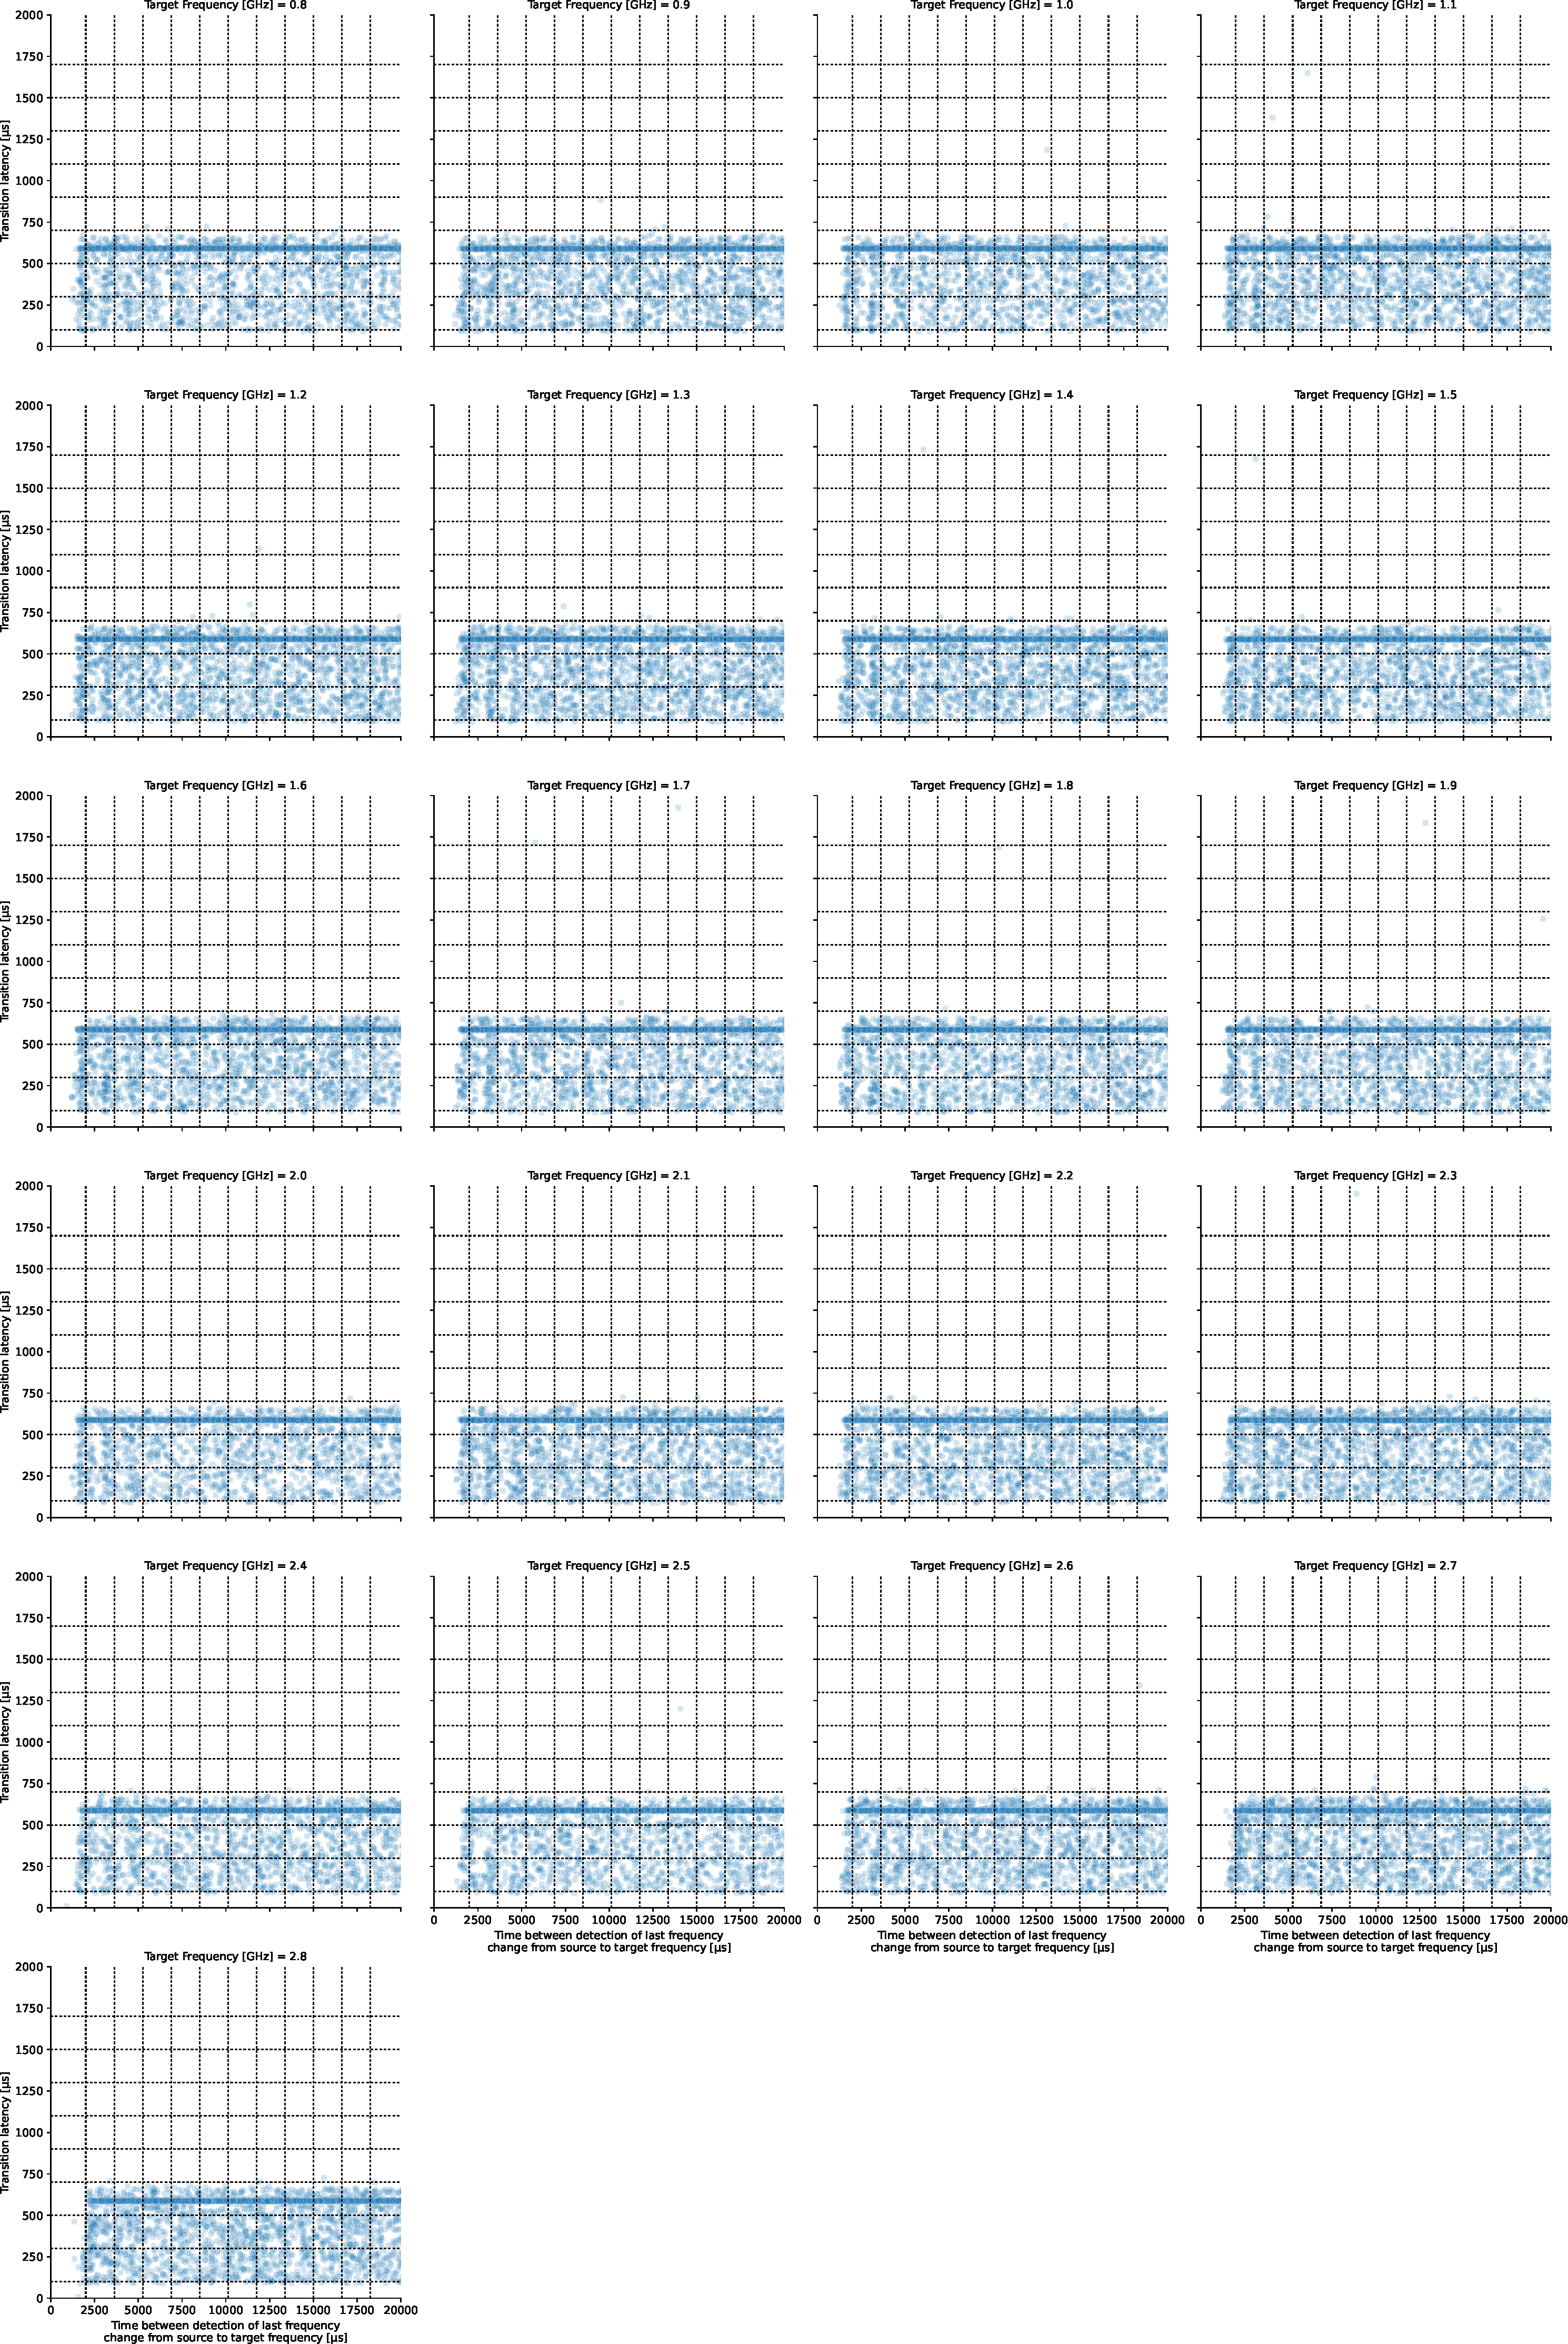
\includegraphics[width=\columnwidth]{fig/ftalat_scatter_wait_transition_latency_hati_source_2.9.pdf}
    \caption{Dependance of the time between the detection events of transitions from \SI{2.9}{\GHz} to \SI{0.8}{}, \SI{0.9}{}, ..., \SI{2.9}{\GHz}. For better lines for bins of size \SI{1625}{\us} and \SI{200}{\us} have been included for the x and y-axis respectively.}
\end{figure}